\begin{quote}
	\textit{``Amplified, shielded, channeled, prosthetized, simulated, stimulated, irritated - our sensorium is more mediated today than ever before. Yet it bothers us less. The cyborg model of the 1980s and the virtual dreams of the 1990s have evolved into a twenty-first-century `comfort zone', in which the prosthetic and supplemental are habitual.''}
\end{quote}
\hfill \textit{The Mediated Sensorium, Caroline A. Jones}
\\
\\

%=========================================================================================================

\label{chapter-eval-1}

The development of the Mirrorshades platform was driven both to investigate mobile parallel reality systems as a concept in general and to assess their suitability when applied to a particular case study as a new modality for interacting with VR content within the context of a cultural heritage site. For this purpose evaluation of the platform firstly addressed its reception compared to a `traditional' VR cultural heritage experience before studying reactions and preferences toward different parallel reality implementations with regards to the default view and transition styles provided.

%=========================================================================================================

%Final video
%\url{https://www.youtube.com/watch?v=UsDRPjDwr8A}
%screenshots

%=========================================================================================================

\section{Overview}

The Mirrorshades parallel reality platform was evaluated in two stages; the first assessed the utility of Mirrorshades as a mobile parallel reality platform in comparison to existing VR techniques used within a virtual heritage context, while the second investigated participants' preferences and reactions toward different transition styles, in order to inform further parallel reality implementations. A combination of qualitative and quantitative data were collected for both stages, as the nature of investigation the experience of the platform is such that purely quantitative data are not sufficient to gain true insight into the experiential aspect, but are nonetheless useful to corroborate, or rebut, qualitative responses and observations.

Participants were sourced by adverts disseminated via an internal university memo system, which sends email to all registered staff and students each week. The advert appeared for several consecutive weeks. Participants were invited to take part in a \textit{``virtual reality study \ldots\ investigating different ways of switching your view between your real surroundings and a virtual environment''}. Participation was incentivised by a prize draw to win Amazon vouchers. This approach was adopted instead of sourcing participants from within the OVW group and wider (computer science) department, as participants with a heightened knowledge \&/or interest in the technology underlying the platform were expected to skew results by paying conscious attention to the system and its implementation rather than the actual experience of using the system. In total 17 participants, 10x male and 7x female, with a mean age of 23.1 years and a standard deviation of 4.9 years, took part in the user studies, each lasting 20-30 minutes. All studies took place at St Salvator's chapel during afternoon hours, with the chapel open to the general public.

\begin{figure}[ht]
	\begin{center}
		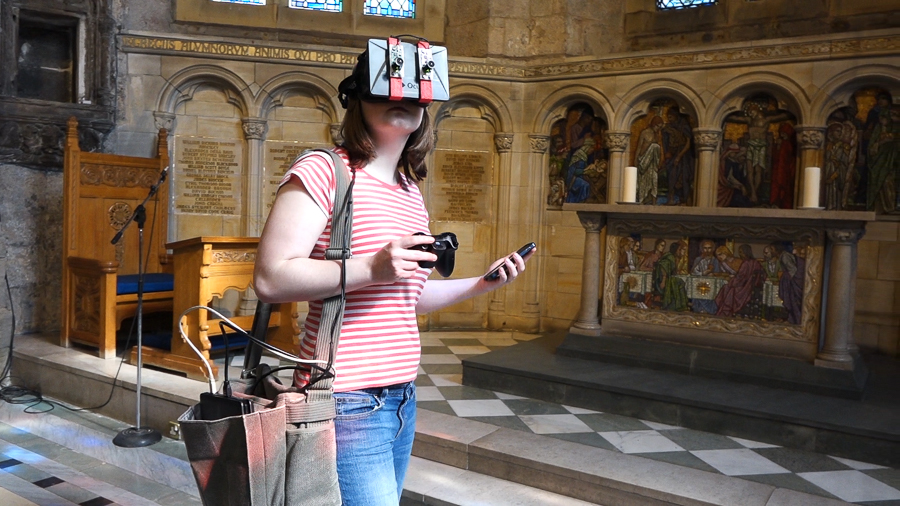
\includegraphics[width=\linewidth]{participant-f.jpg}
		\caption{Participant using Mirrorshades in user studies at St Salvator's chapel.}
		\label{participant-f.jpg}
	\end{center}
\end{figure}

%=========================================================================================================

\section{Stage 1 - Parallel Reality for Virtual Heritage}

Previously when immersive VR has been employed in virtual heritage scenarios, it has predominantly been implemented as CAVE experiences~\cite{Roussou2002}. Visitors to a museum or visitor centre are presented the opportunity to step into a CAVE, possibly donning shutter glasses or similar apparatus to enable a stereoscopic 3D effect, to experience a VR reconstruction of a location, its contents and actors. Some of these CAVE installations have featured physical control interfaces such as joystick and 3D mouse~\cite{cabral:x3dexperience} and haptic interfaces~\cite{Christou2006}, while others have tracked user movement, whether head only or full body  gestures (such as the OVW group's VTTP platform shown in figure \ref{VTTP_projection.png}). In common among these CAVE experiences is that the VR content they present is experienced with a disconnect to the RW site that it pertains to, as the CAVE itself completely immerses users in VR visuals and does not permit them to see any of their RW surroundings, comparable to the experience of wearing a VR HMD without see-through video functionality. Furthermore, the physical size of a CAVE limits the amount in any particular direction that a user can physically move, even if movement is encouraged due to its use as a control methodology. This presents a hindrance to the on-site comparison of real and virtual content, as it introduces both temporal and spatial separation between a user's experiences of the VR content and the corresponding RW environment.

With the promise of high performance VR HMDs at a consumer price point on the horizon, thanks largely to the rejuvenation in the field effected by Oculus, their use at cultural heritage sites for achieving similar experiences to previous CAVE installations is becoming more plausible and brings with it certain benefits such as a reduction in the physical space required at the site for the installation. The OVW group's experience with presenting both experts and interested amateurs, young and old, with virtual heritage content via Oculus HMDs (see section \ref{virtual-heritage-at-st-andrews}) has been very promising. These interactions have taken place in scenarios similar to those of existing cultural heritage CAVE scenarios; the user remains physically stationary and uses a controller or gestures to move their virtual presence throughout the VR environment, whilst unable to observe their RW environment due to the nature of the HMD isolating them from RW visual stimuli.

In this first stage of the evaluation a comparison is made of this seated style of interacting with VR content at a cultural heritage site wherein VR is experienced in isolation from RW, with both temporal and spatial separation, against the parallel reality style of interaction afforded by the Mirrorshades parallel reality platform, in which VR is experienced in tandem with RW by allowing the user to move around their RW environment and transition at any time into seeing the VR environment from the equivalent vantage point. Participants in this stage of the evaluation thus completed two scenarios wherein they interacted with the RW St Salvator's chapel and its corresponding VR reconstruction;

\begin{enumerate}
	\item \textbf{Seated VR scenario} - Participants experience the RW and VR chapels separately. They navigate the VR chapel from a stationary position, as VR has already come to be employed at cultural heritage sites via CAVE installations and by the OVW group with Oculus HMDs, using the Xbox controller to move around the VR environment observed via the DK1, with the DK1 obscuring their view of the RW chapel around them. Subsequently, they navigate the RW chapel without the DK1 or any associated equipment, in order to pay comparison between it and the VR environment they have just perceived.
	\item \textbf{Parallel reality scenario} - Participants experience the RW and VR chapels in tandem using the Mirrorshades platform. They wear the DK1, holding the Xbox controller in their right hand and the smartphone in their left, with the laptop and control box bundle in a satchel worn over one shoulder (see figure \ref{participant-f.jpg}). Pressing and holding a button on the Xbox controller triggers a transition from RW visual stimuli to VR visual displayed by the DK1.
\end{enumerate}

This first stage of evaluation was designed to ascertain whether applying mobile parallel reality to a cultural heritage scenario results in an improvement in participant engagement and understanding of the relationships between the RW and VR environments, compared to a seated VR cultural heritage scenario. Improvements were expected to result from addressing the problems of spatial and temporal separation inherent with a seated VR scenario by imparting upon the participant the ability to transition at will and with no delay between equivalent vantage points within the RW and VR environments.

%=========================================================================================================

\subsection{Design of the Scenarios}

The scenarios were intended to mimic the style of exploration and interaction that visitors to the chapel usually display, after observing the behaviour of such visitors on several occasions. From these observations, a common pattern of behaviour emerged: visitors enter the chapel from the North/West corner then proceed to walk Eastwards along the nave, pausing to look around after passing through the rood screen, before continuing along the nave toward the altar. They then pause in front of the altar upon reaching the end of the pews and then walk North toward the tomb where they pause again to inspect it. Participants in this first stage of the evaluation process were instructed to imagine that they were performing a similar visit to the chapel and to follow a similar path, pausing after the rood screen, at the end of the pews and in front of the tomb to look around their environment(s) in more detail, however they were encouraged to stop and look around at any times/positions that they wished and not to feel restricted to the described path and locations - the intent of the scenario was to encourage a natural style of exploration despite the unusual situation of making use of bulky VR hardware, rather than to restrict them to an `on rails' experience. Participants were shown the map included as figure \ref{chapel-path} (oriented North upwards) to help visualise the scenario.

\begin{figure}[h]
	\begin{center}
		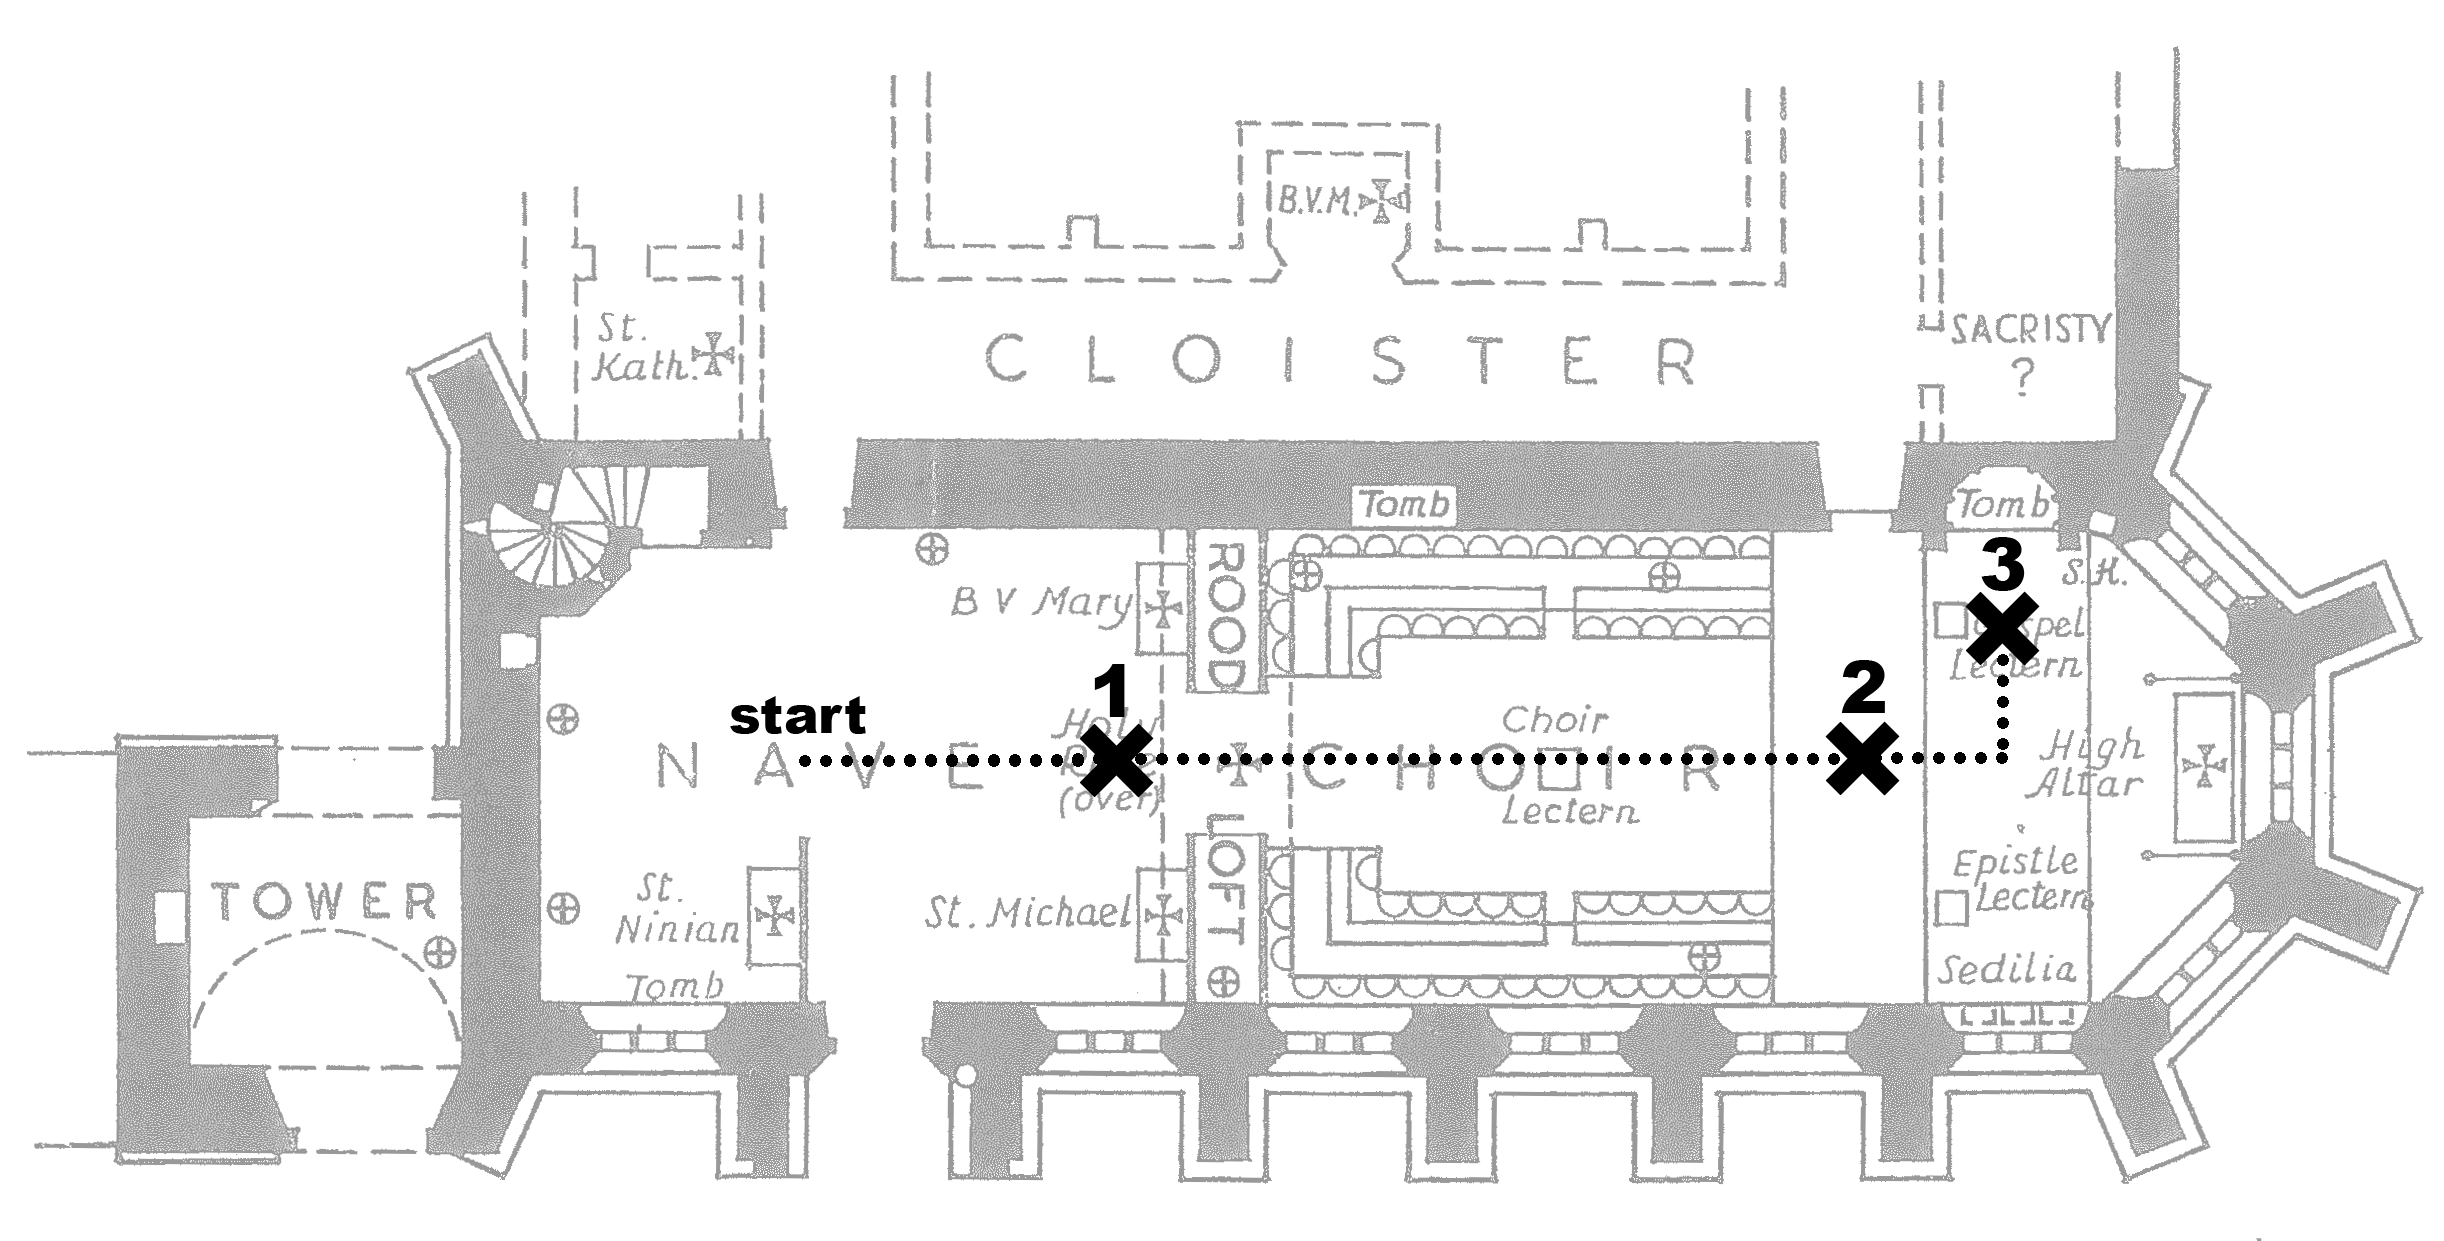
\includegraphics[width=.6\linewidth]{chapel-path.png}
		\caption{Path and positions within St Salvator's chapel that participants were instructed to roughly follow and attend to (oriented North upwards).}
		\label{chapel-path}
	\end{center}
\end{figure}

In the seated VR scenario participants interacted with the VR chapel using the DK1 and Xbox controller while seated. After completing the path in the VR chapel, they removed the DK1 and walked through the real chapel. This behaviour alludes to how VR has previously been applied to cultural heritage sites such as St Salvator's chapel, where visitors have the opportunity to experience a CAVE or seated HMD based reconstruction of the site either before or after having explored the RW site. In the parallel reality scenario, they walk roughly the same path, but this time with the ability to transition at any time between viewing the RW chapel and the VR chapel from the equivalent vantage point.

In the parallel reality scenario participants had access to a single transition style, the transition with linear interpolation (see section \ref{transition-with-linear-interpolation}), triggered by pressing and holding the \texttt{A} button on the Xbox controller. As mentioned in section \ref{initial-testing}, this transition emerged as the `favourite' during initial tests within the OVW group, and as such it was chosen as the only transition style for the parallel reality scenario in this first stage of evaluation wherein the focus of the investigation is upon comparing the parallel reality scenario to a seated VR experience and not upon gleaning details of the merits and drawbacks exhibited by different implementations of parallel reality. The default view on the DK1's screen was 100\% RW with the transition causing a change to 100\% VR, a situation visualised upon the combined Milgram/Waterworth model in figure \ref{focus-locus-sensus-with-virtuality-continuum-with-transition}.

Before taking part in the two scenarios, participants were given the opportunity to familiarise themselves with the DK1 by spending a few minutes interacting with Oculus' `Tuscany' demo\footnote{\url{https://share.oculus.com/app/oculus-tuscany-demo}}. This demo was developed by Oculus themselves and is distributed with the Rift Unity integration package. It represented at the time a very polished and stable DK1 experience, ideal for introducing inexperienced users to HMD based VR. It was used to give participants an opportunity to acclimatize to the Rift (some people react badly to a first VR HMD experience, with feelings of nausea) in order to reduce skewing their subsequent experiences with the St Salvator's chapel model due to drastically different levels of familiarity with the DK1 between the two scenarios.

%=========================================================================================================

\subsection{Evaluation Techniques}

Comparison of the seated VR scenario against the parallel reality scenario is facilitated by the collection of a variety of both qualitative and quantitative data. All participants completed a pre-task questionnaire which provides calibration for other data by enquiring about age, gender identity, previous experience with VR HMDs and whether they had previously visited St Salvtor's chapel, both RW and VR (the RW chapel is open to the public and a version of the VR reconstruction is publicly accessible via the OVW group's OpenSim grid\footnote{\url{openvirtualworlds.org}}). The System Usability Scale (SUS)~\cite{Brooke1996} was used to provide a basic comparison between the usability of the two scenarios, while a 12-item Likert-type questionnaire (included as appendix \ref{appendix-12-item-likert-type-questionnaire-stage-1}) was used to collect opinions on more specific aspects of the experience of both scenarios. At the end of the session, after completing both scenarios, participants were engaged in a short structured interview (prompts included as appendix \ref{appendix-interview-questions-stage-1}) in order to allow them to elaborate upon their experience in a more free form manner. Finally, in addition to the DK1 visuals being recorded via ShadowPlay, log data were collected during both scenarios, capturing the information detailed in table \ref{logdatatable} to file at regular intervals for processing and visualising via R.

\begin{center}
\begin{longtable}{ l  p{8cm} }

\toprule

\textbf{Field} & \textbf{Description} \\

\midrule

\texttt{<frame number>} & Incremented with each frame pushed to the DK1, starting at 0 when the Unity application is run. \\

\midrule

\texttt{<timestamp>} & According to the laptop's internal clock. \\

\midrule

\texttt{<original\_position>} & The position as a Unity \texttt{Vector3} where the participant begins the experiment (as reported by IndoorAtlas). \\

\midrule

\texttt{<position>} & The position as a Unity \texttt{Vector3} where the participant is on this frame (as reported by IndoorAtlas). \\

\midrule

\texttt{<delta\_x>} and \texttt{<delta\_z>} & The difference in the \texttt{x} and \texttt{z} axes between \texttt{<original\_position>} and \texttt{<position>} on this frame. Change in elevation (\texttt{y} axis) is not recorded, as IndoorAtlas does not provide elevation data and the area of St Salvator's chapel used throughout the studies is level. \\

\midrule

\texttt{<left\_rotation>} and \texttt{<right\_rotation>} & The orientation as Unity \texttt{Quaternion} of the two Unity camera game objects. The orientation of these Unity objects is directly tied to the orientation of the DK1, so these values represent the orientation of the participant's head on each frame. \\

\midrule

\texttt{<base\_opacity>} & The maximum opacity of the game objects upon which the camera feeds are rendered. This is how reduced maximum opacity (see section \ref{subsub-baseopacity}) is implemented (by setting this field to a value \textless 1). \\

\midrule

\texttt{<left\_opacity>} and \texttt{<right\_opacity>} & The opacity on this frame of the game objects upon which the camera feeds are rendered. \\

\midrule

\texttt{<auto\_tick>} & Whether a periodic switch is in progress (see section \ref{subsub-periodic}). \\

\midrule

\texttt{<auto\_duration>} and \texttt{<auto\_spacing>} & The interval and duration values of the periodic switching (if applicable). \\

\midrule

\texttt{<framerate>} & An estimate of the current frame rate (frames per second). \\

\midrule

\texttt{<A\_button>}, \texttt{<B\_button>} and \texttt{<right\_trigger>} & The current values of these inputs on the Xbox controller. For the \texttt{A} and \texttt{B} buttons this is binary, either pressed or not, while for the trigger it is a numeric value representing the amount that the trigger is being depressed. \\

\bottomrule
\caption{Log data captured during Mirrorshades evaluations.}
\label{logdatatable}
\end{longtable}
\end{center}

%=========================================================================================================

\section{Stage 1 Results}

A total of 6 participants completed the stage 1 investigation;
\begin{itemize}
	\item Age ranged from 21 to 26, with a mean of 23.3 and a standard deviation of 1.86
	\item 3x identified as male and 3x as female
	\item All reported previous experience with a games console controller
	\item 1x reported previous experience with a HMD
	\item 2x reported having previously visited the chapel
	\item None had previously experienced the virtual chapel
\end{itemize}

%=========================================================================================================

\subsection{SUS}
As expected the parallel reality scenario scored slightly lower on SUS than the seated VR scenario (see figure \ref{sus.png}). The cumbersome nature of the hardware was expected to have this impact upon SUS scores, with the parallel reality scenario averaging lower than the seated VR scenario. Participants who were able to overcome this cumbersomeness were expected to respond more favourably to the parallel reality scenario than those who could not and the small size of the discrepancy between the two results indicates that most participants did not find the cumbersome nature of the parallel reality scenario a substantial detractor to their experience.

\TwoFig{1/sus.png}{Stage 1 evaluation SUS results.}{sus.png}
       {1/post_task_questionnaire_boxplot.png}{Stage 1 evaluation Likert-type questionnaire results.}{post_task_questionnaire_boxplot.png}

%=========================================================================================================

\subsection{Likert-type Questionnaires}

One participant did not complete the Likert-type questionnaires. Coincidentally this participant was also the only one to have reported previous experience with a HMD in the pre-task questionnaire, so the Likert-type questionnaire responses wholly represent participants with no prior HMD experience. With the resurgence of interest in HMD based VR in recent years the number of developers and enthusiasts with HMD experience is climbing. However until the first commercial VR HMDs are released and begin to permeate gaming and media consumption audiences the situation captured by these questionnaire results, where all visitors to a cultural heritage site had no previous HMD experience, should be considered representative of the general public. When considering the responses to the Likert-type questionnaires (see figure \ref{post_task_questionnaire_boxplot.png}) for the first stage participants several observations can be made.

Participants generally found the parallel reality scenario to be more enjoyable and more rewarding than the seated VR scenario, with the former allowing them to more easily perform comparisons between features from the past and present. Participants felt that they better understood what the chapel was like in the past after the parallel reality scenario, compared to the seated VR scenario, however both scenarios scored equally low for participants thinking that they did not notice differences between RW and VR. The parallel reality scenario led to a greater awareness of both environments, a greater sense of `being there' and a greater sense of `being in the past' than the seated VR scenario.

The visual quality of the headset was perceived as being worse in the parallel reality scenario. Whilst the visual quality of the VR visuals was identical in both scenarios, this result is presumably because during the parallel reality scenario the participants were viewing the RW environment upon the DK1's screen via the cameras, with much lower visual acuity than in the seated VR scenario where they observed the RW environment unmediated when subsequently walking through the chapel without the DK1.

It is worth noting that although the parallel reality scenario scored lower than the seated VR scenario in SUS, both scenarios scored highly in question 2 (\textit{``It was easy to compare features from the past and the present''}) and low in question 8 (\textit{``I would have preferred a conventional computer monitor''}).

%=========================================================================================================

\subsection{Interview Transcripts}

Studying the structured interviews that took place after participants had completed both scenarios (interviews were recorded and subsequently transcribed) provided a wealth of qualitative feedback.

All participants said that the parallel reality scenario was more engaging than the seated VR scenario, even though 2x participants said that they preferred the seated VR scenario overall. Of those that said they preferred the seated VR scenario, one did not find it comfortable to walk while wearing the DK1 and the other reported gaining a better understanding of the past from the traditional VR scenario. The participant who found it uncomfortable to walk while wearing the DK1 was notably taller than all of the other participants in this stage. This is worth mentioning as the `height' of the virtual cameras in the VR reconstruction was fixed with reference to the UK average height of 5 feet 9 inches and was not changed to account for different participant heights, as this would have required lengthy recalibration for each and every participant. For a participant of average height, the discrepancy between their RW viewpoint and their VR viewpoint was minimal, however for a particularly short or particularly tall participant this discrepancy would have been much greater and may have contributed to the discomfort of walking with the DK1, as each transition between RW and VR would have resulted in a perceptible shift in height of the viewpoint. Those that said that they preferred the parallel reality scenario alluded to the immediacy of comparison between RW and VR as a contributing factor.

Twice as many participants reported that the parallel reality scenario made it easier to spot differences between RW and VR as reported that the seated VR scenario made it easier, with 4 out of 6 participants reporting noticing differences between RW and VR in the parallel reality scenario that they did not notice in the seated VR scenario. In particular the different position of the rood screen was mentioned by several participants, one participant who didn't notice the different position during the seated VR scenario commenting that the parallel reality scenario made it \textit{``blatantly obvious''}, while another participant was able to list multiple differences that s/he had spotted in the parallel reality scenario that they had not noticed in the seated VR scenario. One participant directly mentioned then confirmed that immediacy of comparison between RW and VR was the enabler of spotting more differences, another mentioned that with the seated VR scenario it was not clear that you were \textit{``trying to look into the past''} but in the parallel reality scenario it was obvious because \textit{``you can see the differences''}, while another directly said that s/he preferred the parallel reality scenario because \textit{``it was easier to compare and contrast between the real world and the virtual one''}.

The quality of the cameras was mentioned as a source of negativity by one of the participants who answered that the seated VR scenario made it easier to spot differences between RW and VR, with another participant specifically mentioning that a higher \textit{``resolution''} was needed.

The one participant to report experiencing motion sickness elaborated that it was worse when using the DK1 in the seated VR scenario than when walking with the DK1 in the parallel reality scenario, because \textit{``sitting down and moving around feels weird''} (a reference to moving throughout the VR environment using the Xbox controller whilst physically stationary sitting on a chair). This observation alludes to the notion of physical embodiment improving a VR experience, by demonstrating the opposite position of restricted movement and a lack of matching embodiment worsening a VR experience.

With regards to movement in the parallel reality scenario, the accuracy and especially the lag of the indoor positioning was cited by one participant as needing work, because it \textit{``caught me off guard twice''}. From watching the ShadowPlay recorded videos from the parallel reality scenario, it is clear that in many cases the participants would trigger a transition to VR visual stimuli only to find that their VR position had not yet `caught up' with their RW position. This behaviour caused by the lag in IPS data was foreseen when considering the update frequency requirement of the IPS provision for the Mirrorshades platform (see section \ref{ips-requirements-for-mirrorshades}) however it was not expected to have as detrimental an effect as was expressed by the participants.

%=========================================================================================================

\subsection{Log Data}

For the seated VR scenario log data were recorded while each participant was engaging with the VR chapel in the seated position and using the Xbox controller to navigate the VR environment. For the parallel reality scenario log data were recorded throughout the whole scenario, such that data are available for both the periods in which they were observing the RW chapel via the DK1 and cameras in addition to the periods in which participants were observing the VR chapel. As such, several comparisons can be made between these sets of data in addition to considering the data as a whole. Within the parallel reality scenario, comparisons can be made between the periods that participants were observing RW and the periods that they were observing VR. Between the seated VR scenario and the parallel reality scenario, comparisons can be made between the VR section of the seated VR scenario and the periods that participants were observing VR in the parallel reality scenario. Log data were not captured for participant 2, nor were they captured for the seated VR scenario for participant 5.

%It was expected that the cumbersome nature of the parallel reality scenario in terms of the hardware that needed to be carried by the participant and the reduced quality of viewing the RW environment via the cameras would have a noticeable restrictive effect upon participants' movement (both in terms of their position and the orientation of their head) in the parallel reality scenario compared to the VR section of the traditional VR scenario, which would be evident from these log data.

\subsubsection{Comparing traditional and parallel reality scenarios}

When looking at either scenario's data (the VR section of the seated VR scenario and both RW and VR periods of the parallel reality scenario) it is immediately evident that participants looked to their sides and turned their heads horizontally (yaw) far more than they looked above and beneath themselves by tilting their heads vertically (pitch). This relationship is shown in figures \ref{1_pitch_yaw_2up.png}, \ref{4_pitch_yaw_2up.png} and \ref{6_pitch_yaw_2up.png}, which show pitch and yaw plotted against time for both the seated VR scenario and the parallel reality scenario, for participants 1, 4 and 6 respectively. With the seated VR scenario on the left of each pair of plots and the parallel reality scenario on the right, the displacement of the blue line representing yaw is substantially greater in both than the displacement of the red line representing yaw.

\begin{figure}
	\begin{center}
	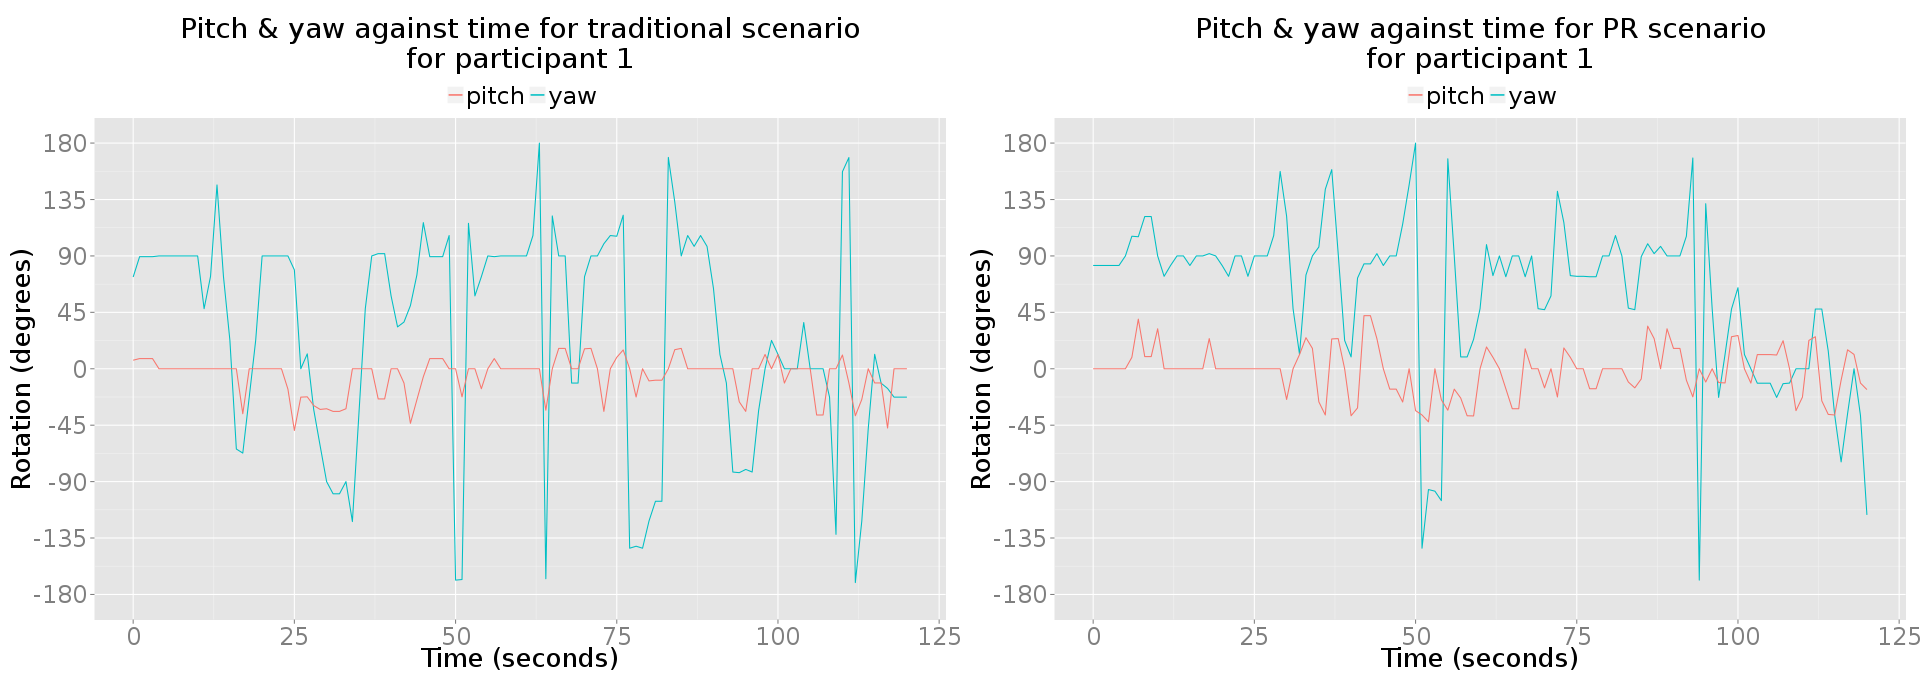
\includegraphics[width=\textwidth]{1/1_pitch_yaw_2up.png}
	\caption{Pitch and yaw against time for participant 1 in seated VR and parallel reality scenarios.}
	\label{1_pitch_yaw_2up.png}
	\end{center}
\end{figure}

\begin{figure}
	\begin{center}
	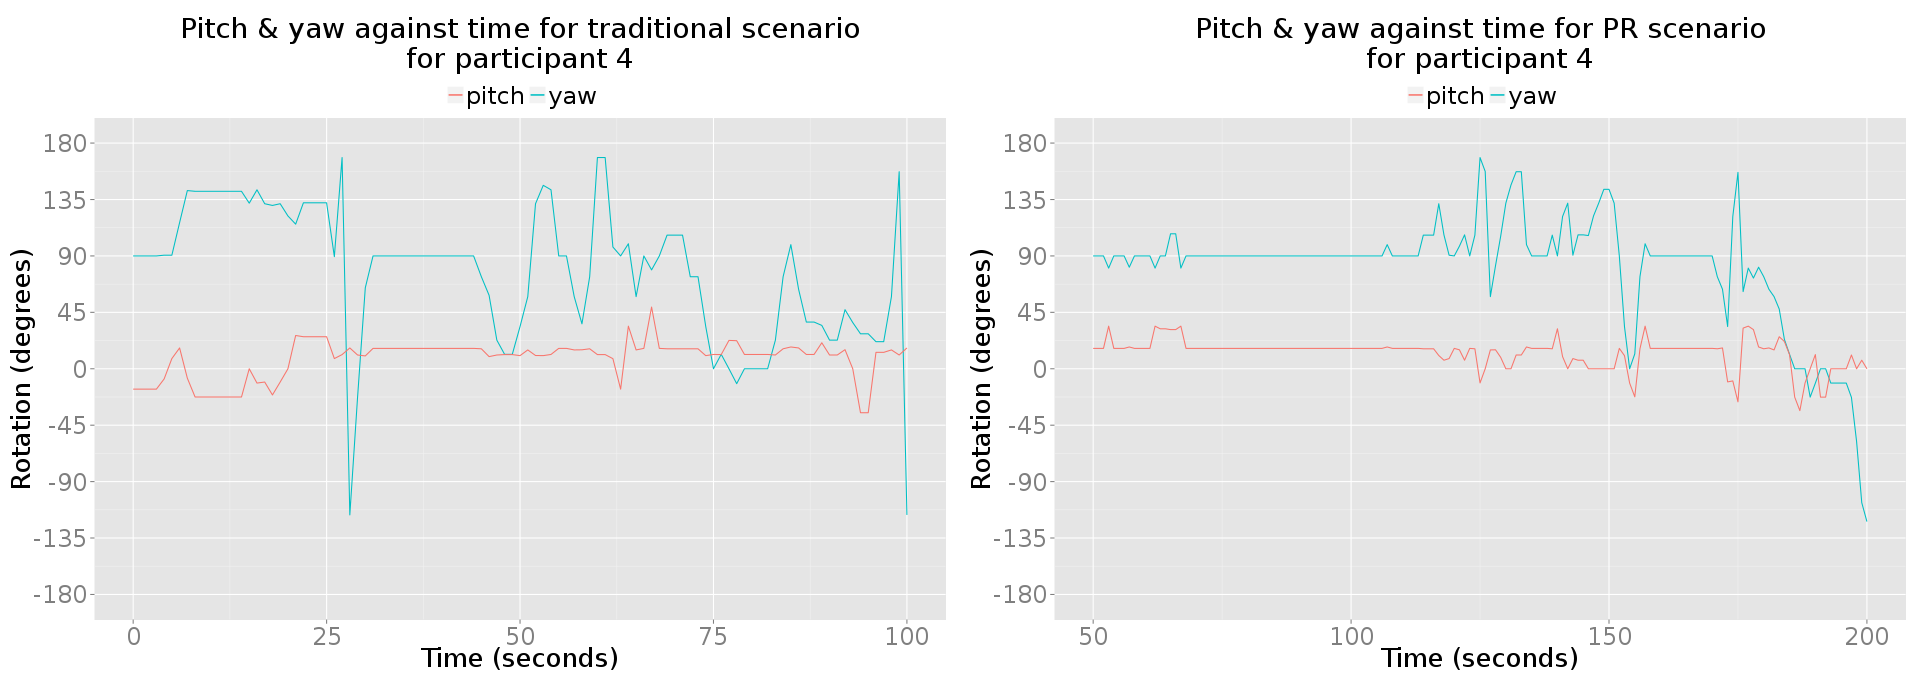
\includegraphics[width=\textwidth]{1/4_pitch_yaw_2up.png}
	\caption{Pitch and yaw against time for participant 4 in seated VR and parallel reality scenarios.}
	\label{4_pitch_yaw_2up.png}
	\end{center}
\end{figure}

\begin{figure}
	\begin{center}
	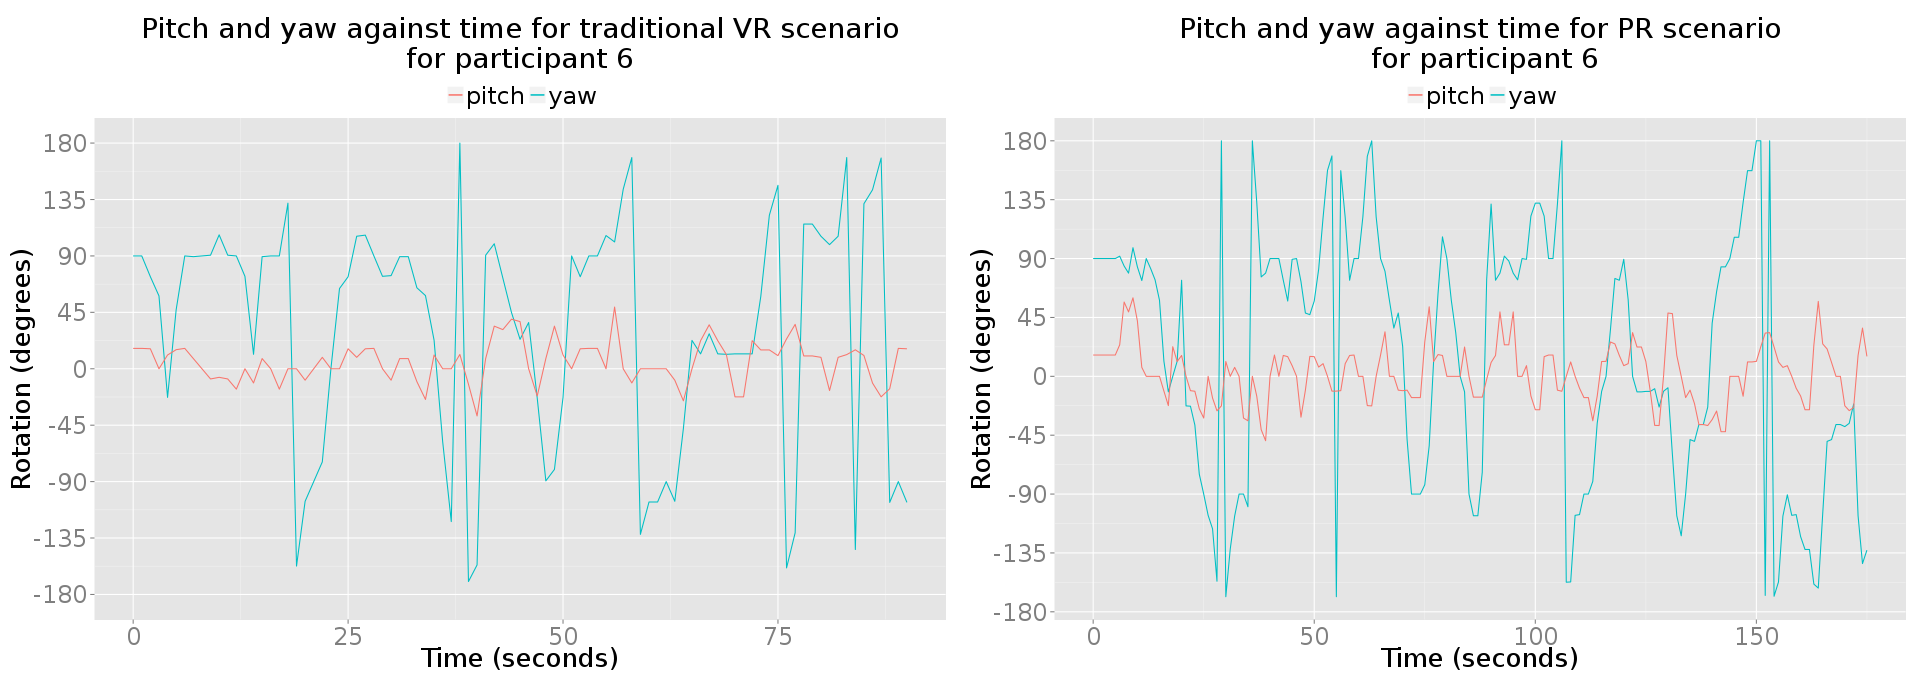
\includegraphics[width=\textwidth]{1/6_pitch_yaw_2up.png}
	\caption{Pitch and yaw against time for participant 6 in seated VR and parallel reality scenarios.}
	\label{6_pitch_yaw_2up.png}
	\end{center}
\end{figure}

This relationship is reflected in calculations of the standard deviation in pitch and yaw across both scenarios, shown by table \ref{sdpitchyawtrad} for the seated VR scenario and table \ref{sdpitchyawpr} for the parallel reality scenario. For every participant for which the data are available, the standard deviation in yaw is substantially higher than that in pitch. This relationship can largely be explained by the simple fact that there is more to observe in the chapel(s) at ground level than above eye level or down at the ground, however with the marked difference in the appearance of the chapel roof (stone in the VR reconstruction, wood in the RW chapel today) a smaller difference between pitch and yaw variance might have been expected for both scenarios.

\begin{table}
\begin{center}
\begin{minipage}[t]{.45\linewidth}
\begin{center}
\begin{tabularx}{\textwidth}{c *{3}{>{\centering\arraybackslash}X}}
\toprule

\textbf{Participant} & \textbf{Pitch (\textdegree)} & \textbf{Yaw (\textdegree)} \\

\midrule

1 & 14.977 & 86.211 \\

3 & 16.684 & 60.545 \\

4 & 10.516 & 53.805 \\

5 & no data & no data \\

6 & 16.172 & 92.416 \\

\bottomrule
\end{tabularx}
\caption{Standard deviation in pitch and yaw for seated VR scenario.}
\label{sdpitchyawtrad}
\end{center}
\end{minipage}
%
\begin{minipage}[t]{.02\linewidth}
\hfill%
\end{minipage}
%
\begin{minipage}[t]{.45\linewidth}
\begin{center}
\begin{tabularx}{\textwidth}{c *{3}{>{\centering\arraybackslash}X}}
\toprule

\textbf{Participant} & \textbf{Pitch (\textdegree)} & \textbf{Yaw (\textdegree)} \\

\midrule

1 & 19.186 & 63.427 \\

3 & 24.228 & 51.666 \\

4 & 11.723 & 44.526 \\

5 & 16.542 & 39.601 \\

6 & 21.999 & 97.122 \\

\bottomrule
\end{tabularx}
\caption{Standard deviation in pitch and yaw for parallel reality scenario (RW and VR periods combined).}
\label{sdpitchyawpr}
\end{center}
\end{minipage}
\end{center}
\end{table}

%=====================

When studying plots of head pitch and yaw against time aligned with plots of distance moved against time, some participants display an aversion to large head movements while moving. Considering participant 1 (figure \ref{1_4up.png}), they seem to have been quite comfortable looking around a lot even while moving in the seated VR scenario, while in the parallel reality scenario their large head movements are close to the periods in which their position was not changing as much\footnote{When looking at these plots it is important to appreciate that lag in the IndoorAtlas data results in a small lateral offset between the position data and the head orientation data, as the latter is unaffected by the lag in the correct reporting and `settling' of the former.}. When looking at the same data plotted for participant 3 however (figure \ref{3_4up.png}), it seems that they were reluctant to perform large head movements while moving in both scenarios, rather than just the parallel reality scenario.

Reluctance to changing head orientation when moving in the seated VR scenario can possibly be explained by something as simple as participant 1 having more experience with video games that present the user with a `first person' perspective in which movement and looking direction are controlled independently. For somebody familiar with this style of control, it is second nature to use one control to change their position whilst simultaneously using another control to change the direction in which they are looking, however for those unfamiliar or inexperienced with such scenarios it is common to observe alternation between movement and looking, something that the OVW group has observed in people interacting with virtual content at various demonstrations using keyboard and mouse, Xbox controller and other control methodologies. For first person shooter (FPS) video games, this simultaneous independent control of head and body is commonly achieved by using keyboard buttons to control body movement while using a mouse to control looking direction, or by using the two separate control sticks of a controller such as an Xbox controller. With the seated VR scenario, the Xbox controller provides control over movement while the head tracker in the DK1 provides control over looking direction by tracking head orientation.

Reluctance to changing head orientation when moving in the parallel reality scenario is most logically explained by participants feeling as though with the reduced visual acuity of their RW environment and the discrepancy in position and environmental objects of their VR environment that they needed to pay more conscious attention to their walking, lest they lose their footing. Upon reaching a location of particular interest and standing still, their willingness to perform larger head movements returns as they no longer have to contend with obstacle avoidance.

\begin{figure}
	\begin{center}
	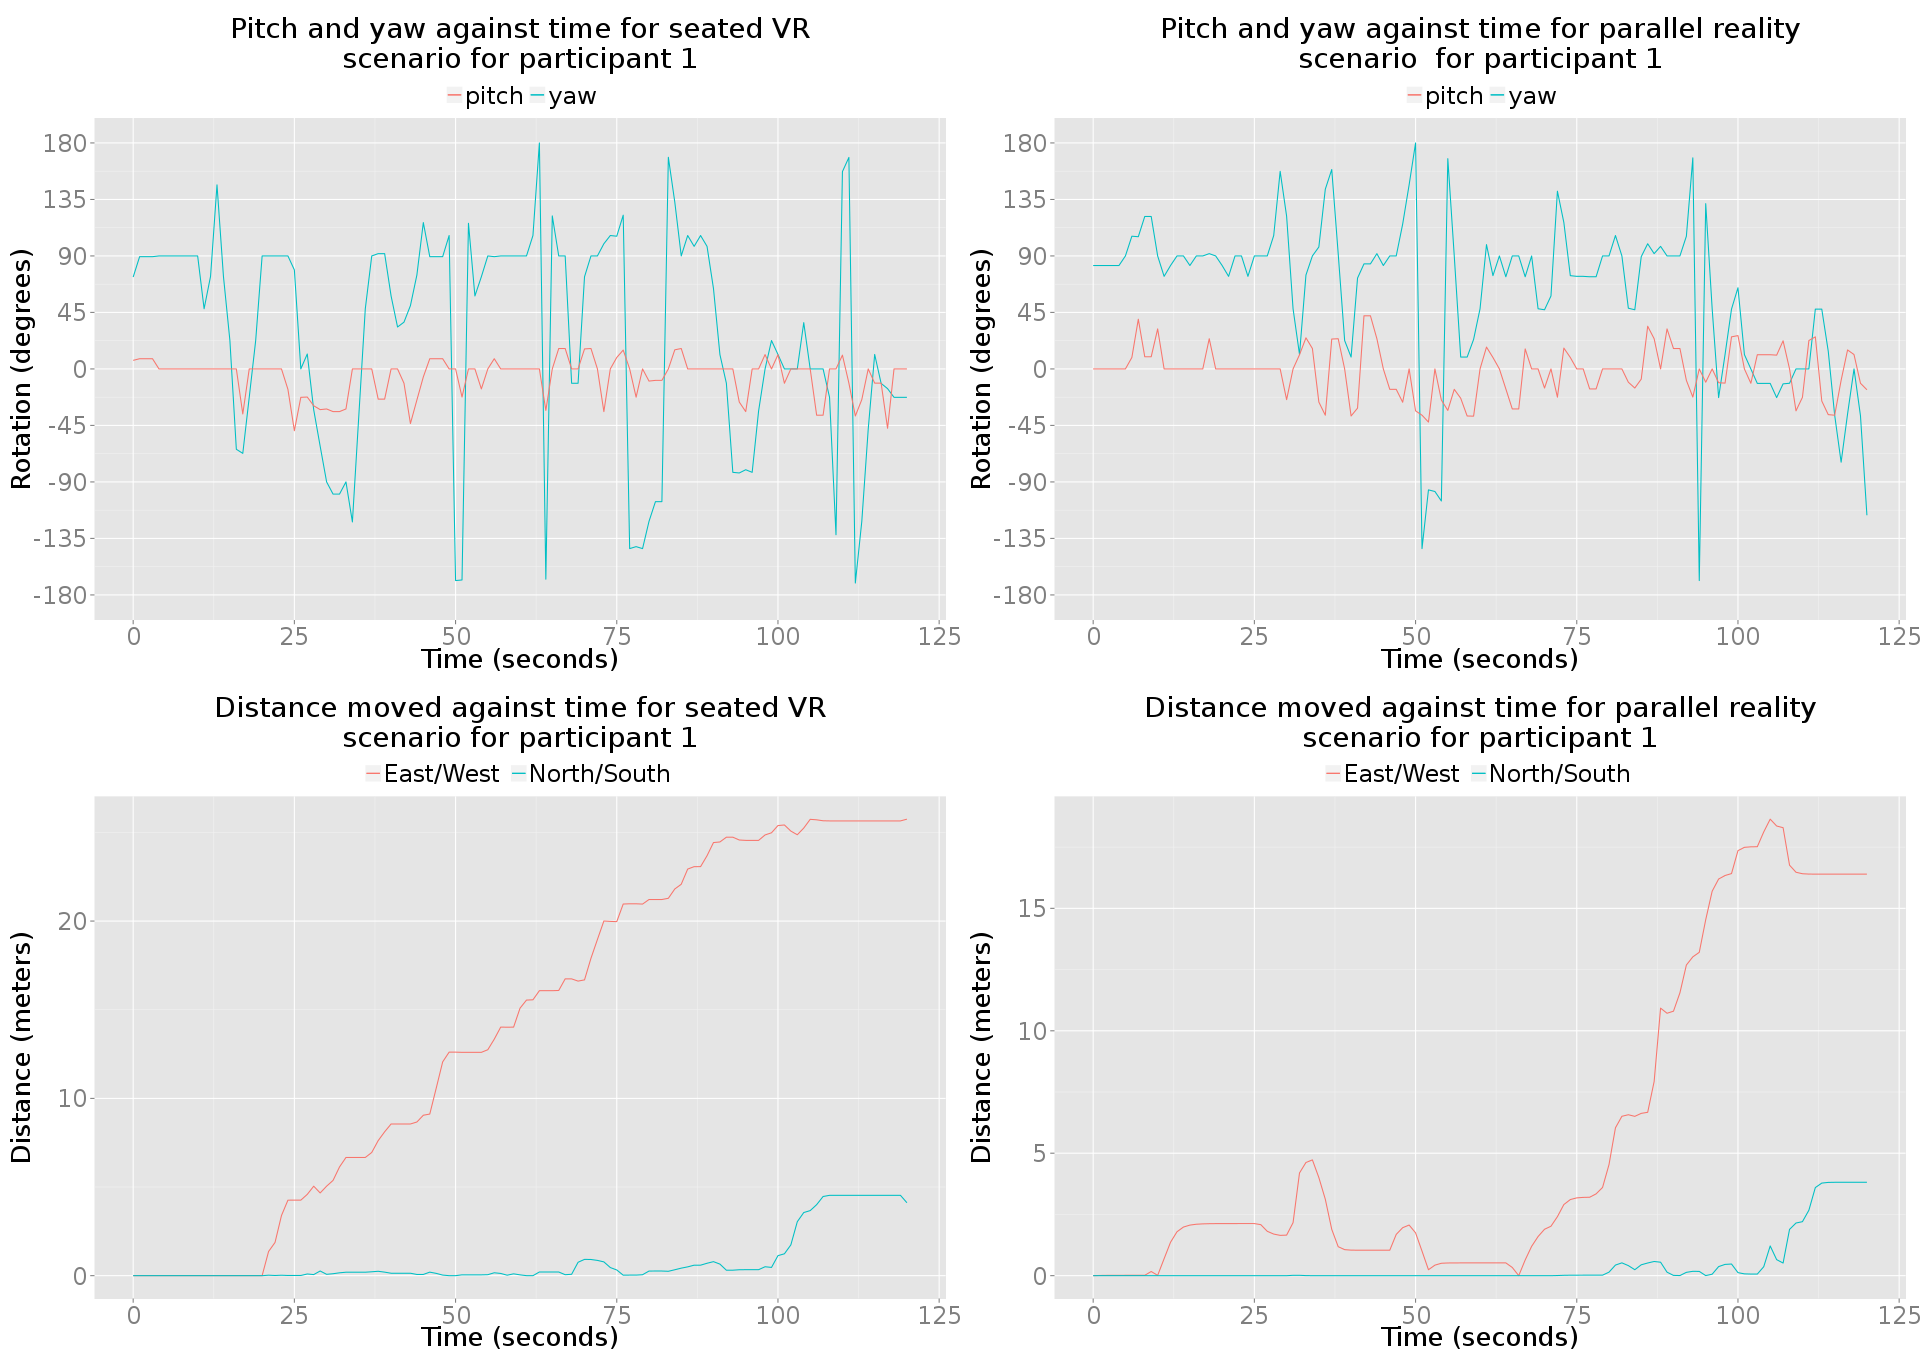
\includegraphics[width=\textwidth]{1/1_4up.png}
	\caption{Pitch and yaw against time, aligned with distance moved against time, for participant 1 in both scenarios.}
	\label{1_4up.png}
	\end{center}
\end{figure}

\begin{figure}
	\begin{center}
	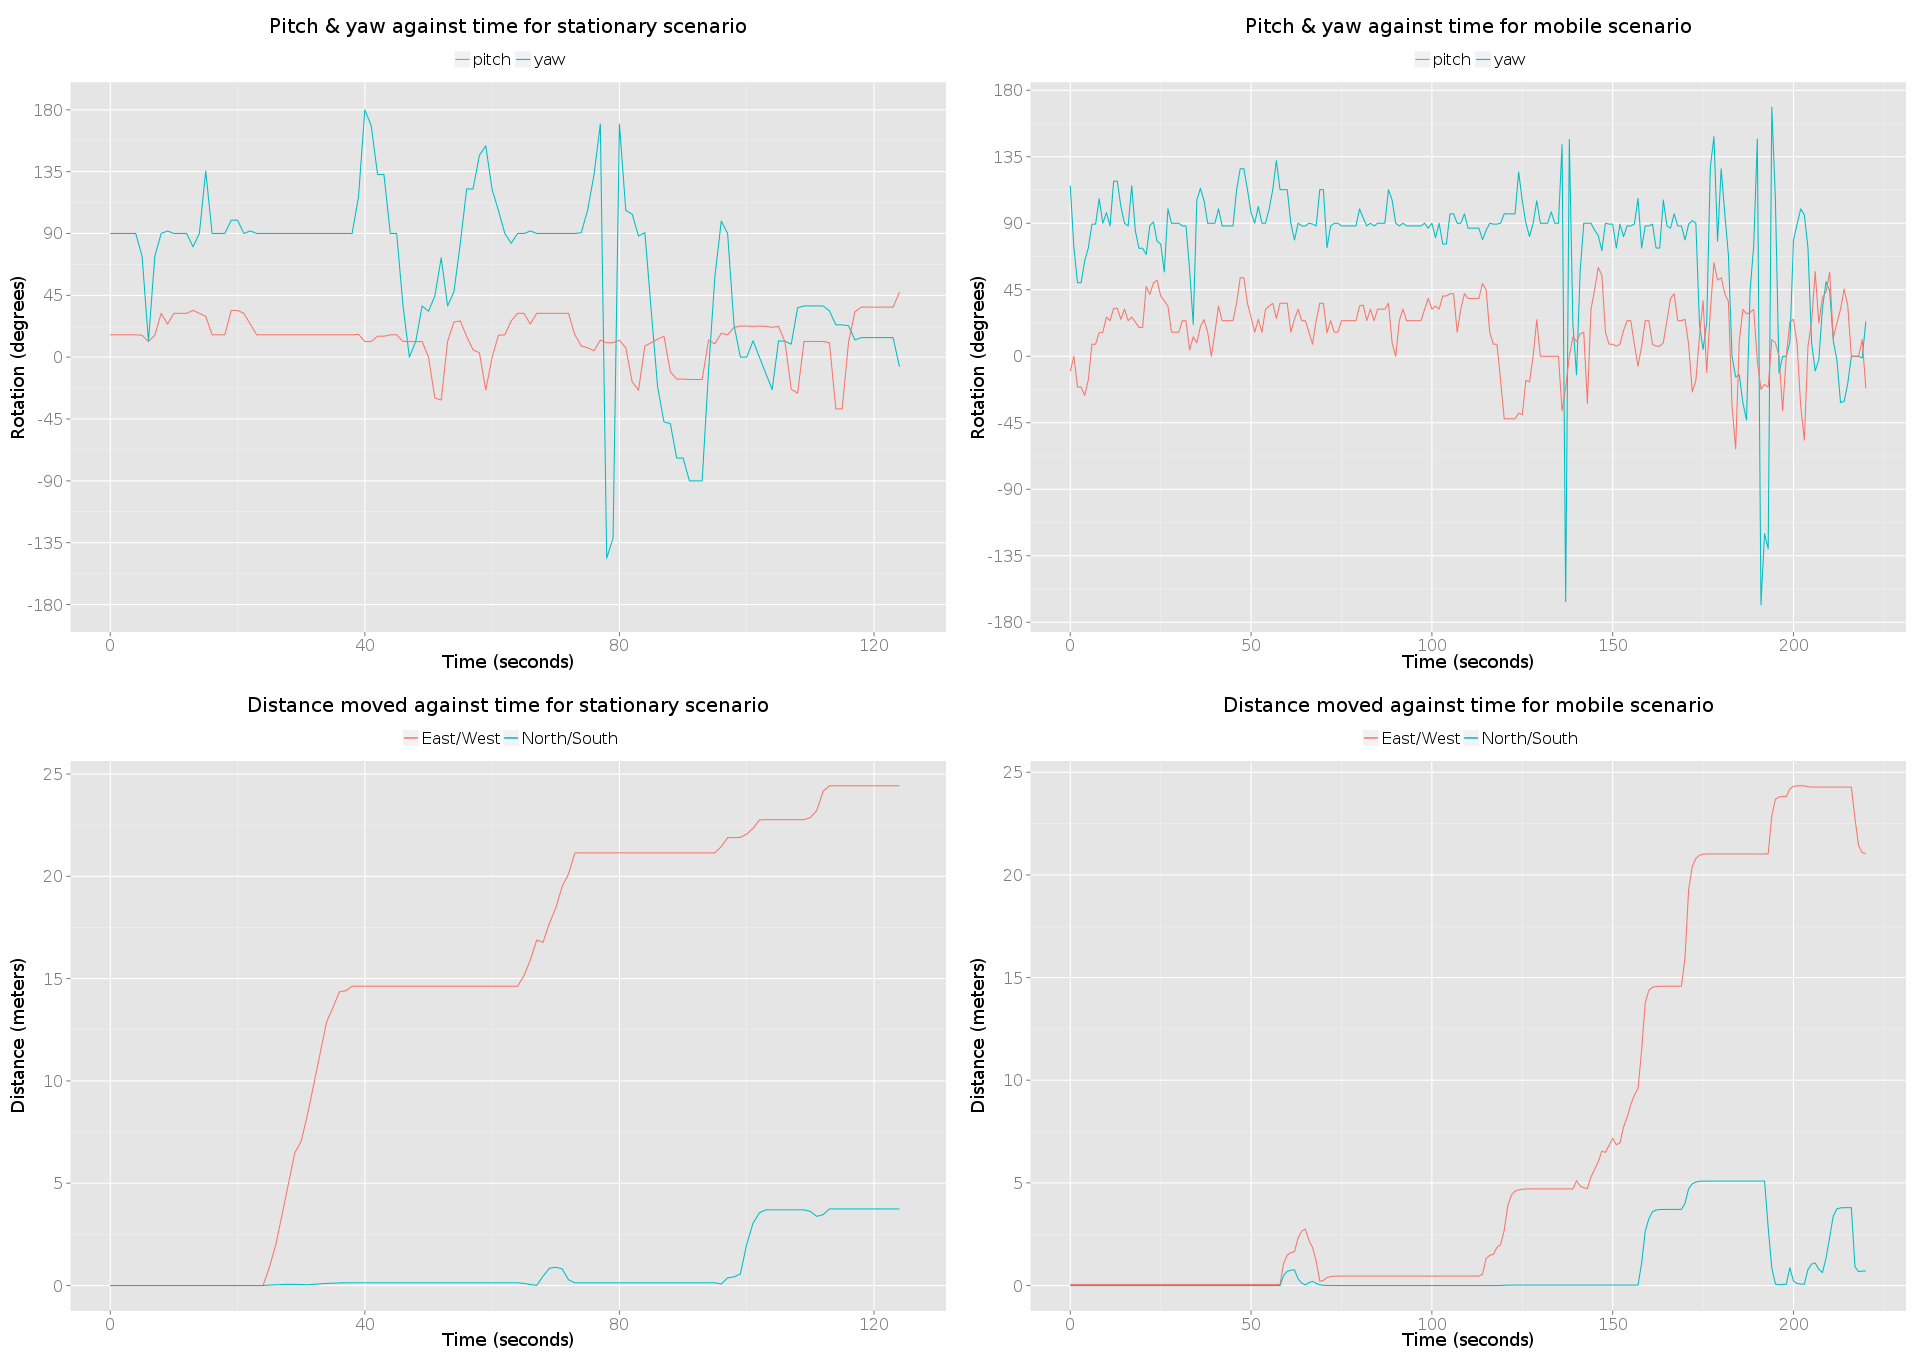
\includegraphics[width=\textwidth]{1/3_4up.png}
	\caption{Pitch and yaw against time, aligned with distance moved against time, for participant 3 in both scenarios.}
	\label{3_4up.png}
	\end{center}
\end{figure}

\subsubsection{Comparing RW and VR periods within parallel reality scenario}

When comparing pitch and yaw data between the RW and VR periods within the parallel reality scenario, it is notable that for some participants there was more variance in the periods in which they were perceiving VR stimuli than in those in which they were perceiving RW stimuli, meaning that they turned their heads more when looking at the VR environment than when looking at the RW environment. This is particularly evident when plotting these pitch and yaw data against time with the periods of RW/VR indicated. Figure \ref{1_pitch_yaw.png} shows the pitch and yaw data for participant 1 during the parallel reality scenario, who prominently displayed this tendency toward greater head movement while viewing VR than RW. The coloured background of the plot indicates which environment the participant was perceiving at that time index; blue for RW and green for VR. Correlation is evident between the most pronounced changes in yaw (red line) and the periods that the participant was observing VR stimuli (green background). As can be seen in figure \ref{3_pitch_yaw.png} this relationship is even more prevalent in the data from participant 3, while the data from participant 5 in figure \ref{5_pitch_yaw.png} still show the relationship but to a lesser extent.

\begin{figure}[h]
	\begin{center}
	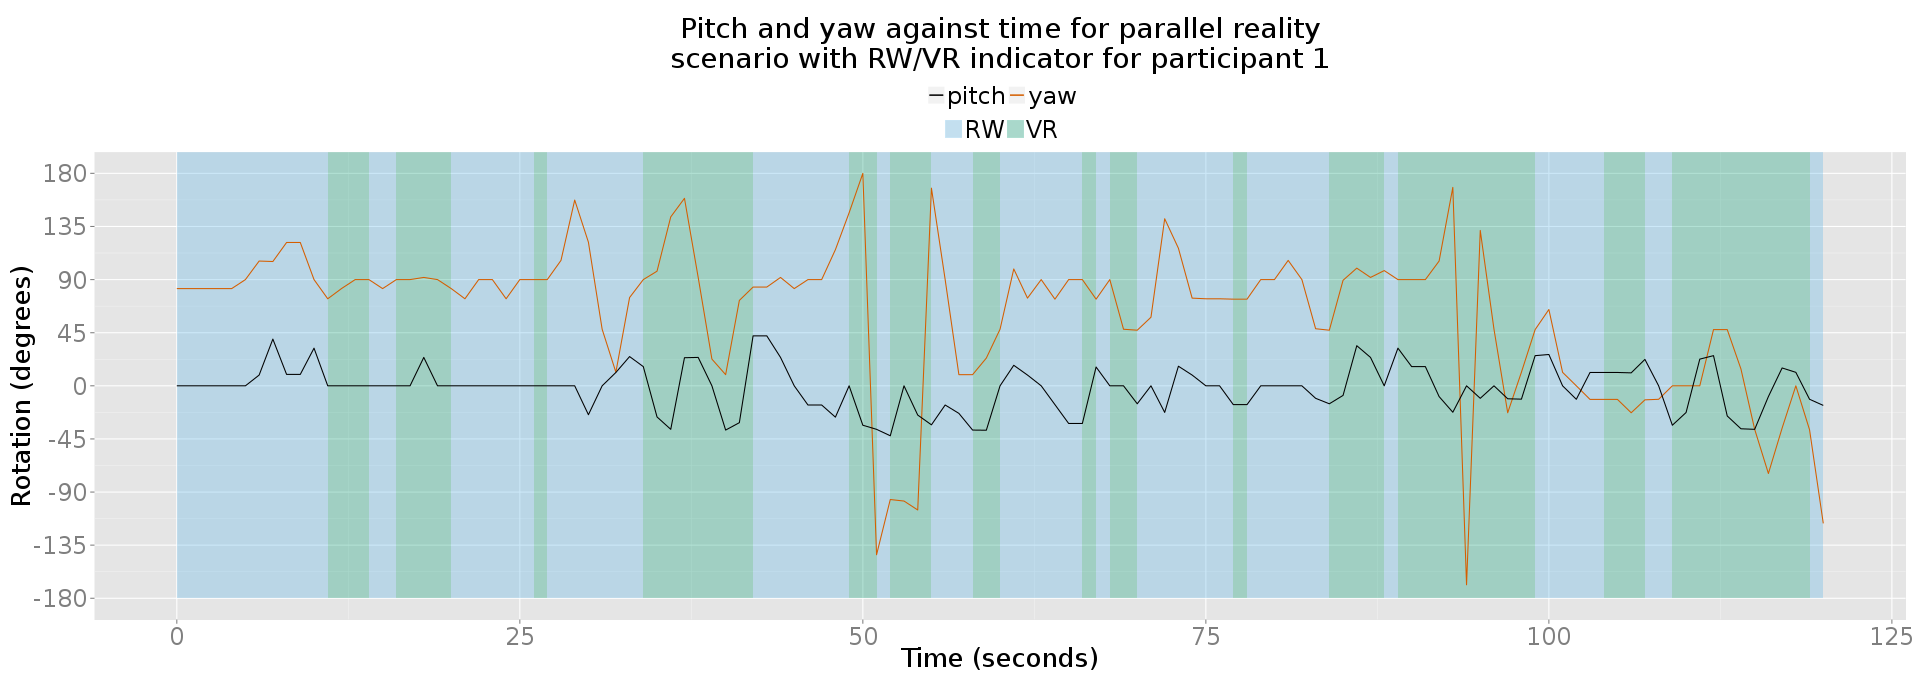
\includegraphics[width=\textwidth]{1/1_pitch_yaw.png}
	\caption{Pitch and yaw against time for participant 1 in parallel reality scenario, showing RW/VR periods.}
	\label{1_pitch_yaw.png}
	\end{center}
\end{figure}

\begin{figure}[h]
	\begin{center}
	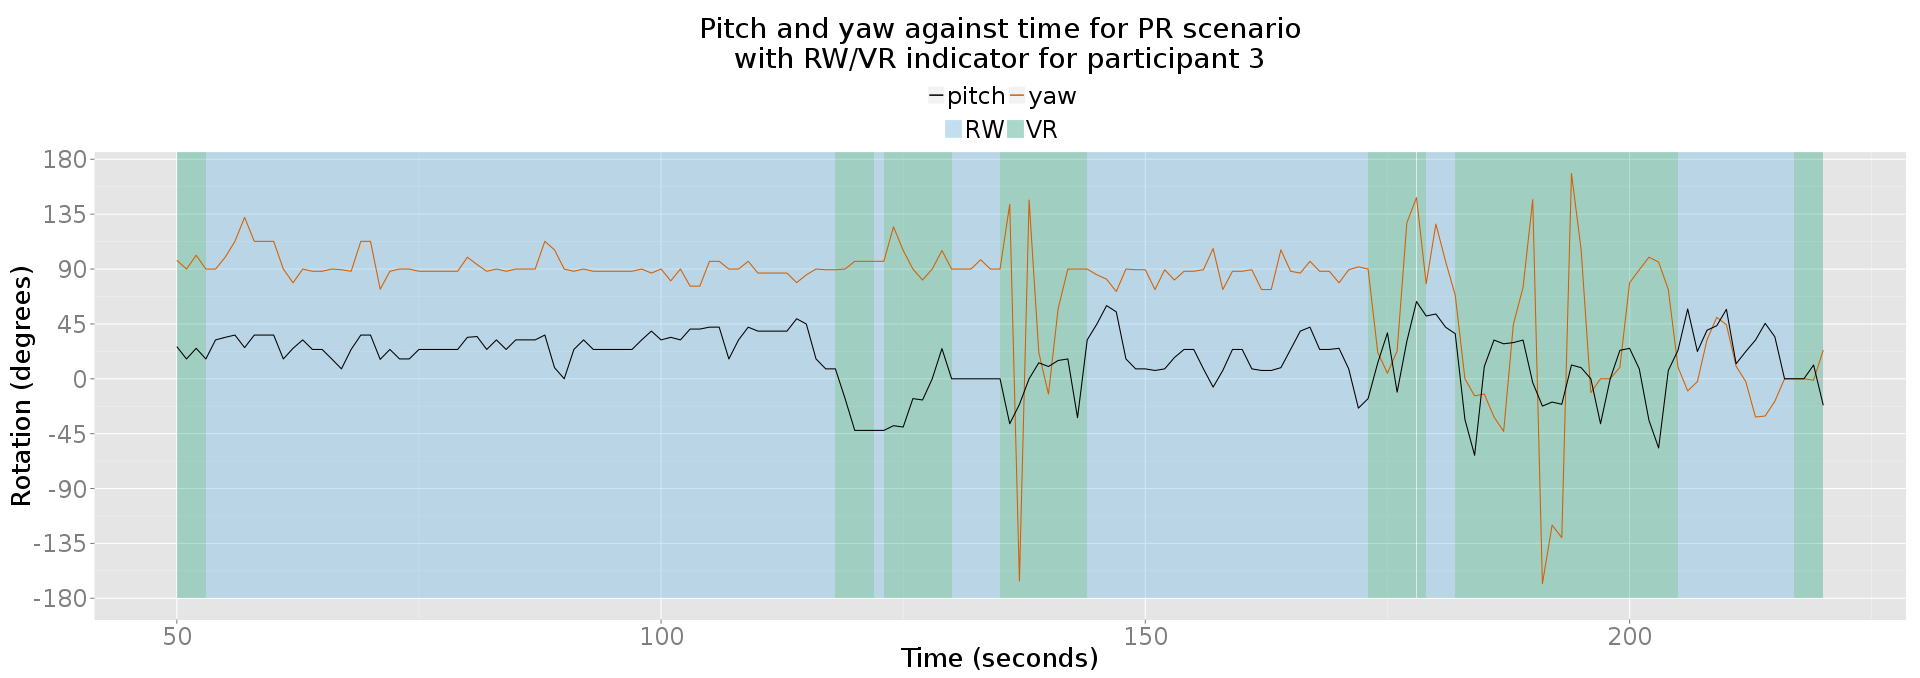
\includegraphics[width=\textwidth]{1/3_pitch_yaw.png}
	\caption{Pitch and yaw against time for participant 3 in parallel reality scenario, showing RW/VR periods.}
	\label{3_pitch_yaw.png}
	\end{center}
\end{figure}

\begin{figure}[h]
	\begin{center}
	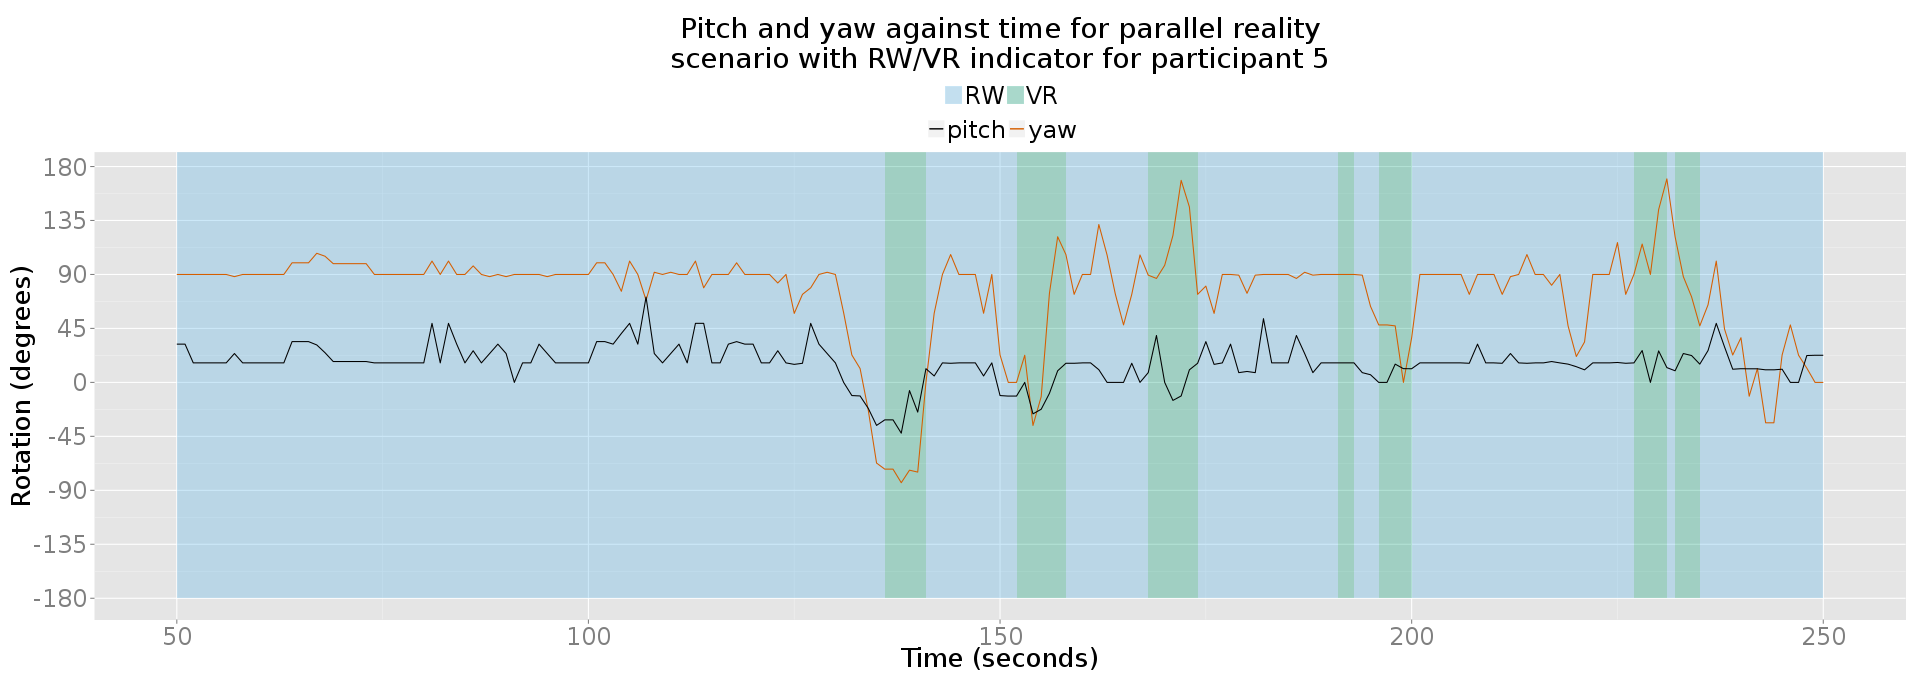
\includegraphics[width=\textwidth]{1/5_pitch_yaw.png}
	\caption{Pitch and yaw against time for participant 5 in parallel reality scenario, showing RW/VR periods.}
	\label{5_pitch_yaw.png}
	\end{center}
\end{figure}

Calculating the mean standard deviation in yaw for both RW and VR periods, weighted by the duration of the periods, shows this relationship more analytically. With reference to the figures in table \ref{sdyawtab} the mean standard deviation in yaw while perceiving VR stimuli is higher than while perceiving RW stimuli for participant 1 (39.887\textdegree\ compared to 25.545\textdegree) and even more so for participant 3 (60.636\textdegree\ compared to 11.702\textdegree). The values are closer for participant 5, due to the initial large delta in yaw just before the first transition into VR at around 130 seconds. Recalculating the weighted mean standard deviation from 150 seconds onwards to exclude this peak gives rise to the values of 36.074\textdegree\ for VR stimuli compared to 17.046\textdegree\ for RW stimuli, which is more in fitting with the impressions drawn from studying figure \ref{5_pitch_yaw.png}. The exception to this observation of correlation between head movement and environment is participant 4, however this participant displayed very restricted head movement throughout both scenarios when compared to all of the other participants.

\begin{table}
\begin{center}
\begin{minipage}[t]{.45\linewidth}
\begin{center}
\begin{tabularx}{\textwidth}{c *{3}{>{\centering\arraybackslash}X}}
\toprule

\textbf{Participant} & \textbf{RW (\textdegree)} & \textbf{VR (\textdegree)} \\

\midrule

1 & 13.325 & 17.554 \\

3 & 12.194 & 24.662 \\

4 & 6.133 & 6.133 \\

5 & 12.193 & 12.797 \\

6 & 15.712 & 15.349 \\

\bottomrule
\end{tabularx}
\caption{Weighted mean sd in pitch for parallel reality scenario.}
\label{sdpitchtab}
\end{center}
\end{minipage}
%
\begin{minipage}[t]{.02\linewidth}
\hfill%
\end{minipage}
%
\begin{minipage}[t]{.45\linewidth}
\begin{center}
\begin{tabularx}{\textwidth}{c *{3}{>{\centering\arraybackslash}X}}
\toprule

\textbf{Participant} & \textbf{RW (\textdegree)} & \textbf{VR (\textdegree)} \\

\midrule

1 & 25.545 & 39.887 \\

3 & 11.702 & 60.636 \\

4 & 18.032 & 15.300 \\

5 & 23.155 & 29.274 \\

6 & 41.717 & 47.440 \\

\bottomrule
\end{tabularx}
\caption{Weighted mean sd in yaw for parallel reality scenario.}
\label{sdyawtab}
\end{center}
\end{minipage}
\end{center}
\end{table}

When considering the amount of time spent perceiving each environment in the parallel reality scenario, several of the participants showed frequent transitioning behaviour where they would perform many transitions and remain perceiving the visual stimuli from each environment for only a few seconds: for participants 1, 4 and 6, the mean times for both RW and VR periods are all between 1.68 and 3.4 seconds. Participant 3 spent longer perceiving each environment with a RW mean of 18.2 seconds and a VR mean of 7 seconds. The outlier is participant 5, with a RW mean of 31.8 seconds and a VR mean of 3.6 seconds; this was the participant who found it uncomfortable to walk while wearing the DK1, so a much longer amount of time spent perceiving RW stimuli is understandable.

\subsubsection{Comparing VR periods of parallel reality scenario to VR section of seated VR scenario}

Comparing yaw from the VR periods of the parallel reality scenario (table \ref{sdyawtab}) against yaw from the seated VR scenario (table \ref{sdpitchyawtrad}) it can be seen that in most cases there is noticeably less yaw change in the VR periods of the parallel reality scenario than in the seated VR scenario, indicating that participants felt more comfortable to perform larger head movements when seated with the DK1 than when standing/walking with it. Observations of participants while they performed the seated VR scenario support this conclusion with several participants twisting their heads right around to look behind them without changing their direction of their virtual `movement', while when walking in the parallel reality scenario participants tended to largely look ahead in the direction their body was facing, performing larger orientation changes by instead turning their whole body before walking in the return direction. As participants were restricted from reorienting their physical body during the VR section of the seated VR scenario (their chair did not swivel) this combined with participants dislike to turning their virtual body with the controller's stick explains why they might perform much larger head movements.

Further comparing head movements between the VR section of the seated VR scenario and the VR periods of the parallel reality scenario, the difference between the magnitude of pitch and yaw is greater in the VR section of the seated VR scenario than in the VR periods of the parallel reality scenario. Comparing these values from tables \ref{sdpitchyawtrad}, \ref{sdpitchtab} and \ref{sdyawtab} this difference exhibits as smaller variance in yaw and roughly unchanged (only slightly increased) variance in pitch for the VR periods of the parallel reality scenario, further indicating that participants were more comfortable to look around themselves more freely in the seated VR scenario than in the parallel reality scenario, leading to less overall head movement in the parallel reality scenario than the seated VR scenario.

%=========================================================================================================

\section{Summary}

The first stage of investigation directly compared a seated VR scenario in which VR content has already begun to be used at cultural heritage sites with the mobile style of interaction afforded by the Mirrorshades platform, addressing both temporal and spatial separation between experience of the real and virtual environments. The Mirrorshades platform has shown itself to be a rewarding new modality for experiencing VR content in a cultural heritage context, improving upon seated VR techniques employable for the presentation of the same content by allowing immediate comparison and contrast between corresponding vantage points in both the RW and VR environments, successfully addressing the hindrance of on-site comparison of real and virtual environments.

Through questionnaire data and interview transcripts participants reported that overall they found the parallel reality scenario to be both more enjoyable and more rewarding than the seated VR scenario, despite the decreased usability and comfort effected by the requirement to don and carry a satchel of hardware and hold devices in both hands. The parallel reality scenario was reported as allowing easier comparison and contrast between RW and VR environments, leading participants to recognise more differences between the two environments and leading to a greater change in and better understanding of the chapel than with the seated VR scenario. The visual acuity afforded by the cameras and both the accuracy and lag of the IPS surfaced as the major detractors to the experience of the parallel reality scenario.

Log data show participants displaying restricted head movement throughout the parallel reality scenario, looking to their sides and above and beneath themselves less when experiencing the VR chapel in the parallel reality scenario than when experiencing the VR chapel in the seated VR scenario. While this restriction does not appear to have been so great that it reduced the utility and enjoyability of the parallel reality scenario to beneath that of the traditional VR scenario, it has been observed by prior investigations~\cite{Slater1998} that there is a significant positive association between reported sense of presence in a VR environment and the amount of body movement, particularly head yaw, displayed by a participant, so reducing the negative impact that a parallel reality system has upon a user's willingness to freely look around them will likely result in beneficial returns, especially when considering that restricted head movement may lead to overlooking interesting aspects of \textit{the both} parallel environments.

%=========================================================================================================
%=========================================================================================================
%=========================================================================================================
%=========================================================================================================
%=========================================================================================================

%\clearpage

\chapter{Informing Parallel Reality Implementation}

%\section{Stage 2 - Informing Parallel Reality Implementation}

\begin{quote}
	\textit{``Let us wander in modernism's cabinet of curiously segmented senses to see what doors we might open to a differently mediated sensorium.''}
\end{quote}
\hfill \textit{The Mediated Sensorium, Caroline A. Jones}
\\
\\

%=========================================================================================================

\label{chapter-eval-2}

The first stage of evaluation into the Mirrorshades platform led to the conclusion that applying a mobile parallel reality system to a cultural heritage scenario provides an experience that is more enjoyable and engaging than a traditional virtual heritage scenario making use of immersive VR presentation via CAVE or static HMD, while also leading participants to a greater understanding of the relationships between the RW and VR content presented to them. While certain drawbacks in the system highlighted by the first stage of evaluation, such as the visual acuity of the video see-through solution and the lag in the IPS, could not be iterated upon before the second stage of evaluation due simply to lack of superior technology, other aspects of the system that affect the overall parallel reality experience could be investigated and these findings used to inform future parallel reality implementations - namely the way that transitions between RW and VR visual stimuli are performed, including whether the default view is 100\% RW or a mix of RW and VR, as participants in stage 1 of the evaluation were furnished with only a single style of transition.

\section{Overview}

Stage 2 of the evaluation was divided into two parts. In the first (stage 2.1), evaluation focussed upon assessing participants' reactions to and preferences toward four different transition styles, while in the second (stage 2.2), evaluation looked at reactions and preferences in response to two different default views comprising RW/VR mixes. In terms of the combined Milgram/Waterworh model, this second stage of evaluation pertains to assessing the effect upon participants' focus of attention (the severity of the `break in presence) and to a lesser extent their sensus of attention, when performing oscillations along the locus of attention axis using different techniques. Stage 2.1 investigates oscillations wherein the default view is 100\% RW, with participants performing oscillations between the RW extreme of the locus of attention axis and other points upon the locus axis (such as in figure \ref{transition-rw-vr-hard.png}), while stage 2.2 looks into oscillations wherein the default view is a mix of RW and VR, limiting how far toward the RW extreme of the locus axis the participant can reach (such as in figure \ref{transition-mix-vr.png}).

While stage 1 of the evaluation investigated the suitability of applying a mobile parallel reality platform to the particular use case of virtual heritage, stage 2, while still within the same virtual heritage scenario, has wider use for informing implementation of parallel reality systems in general and not just within the context of virtual heritage.

\begin{figure}[ht]
	\begin{center}
		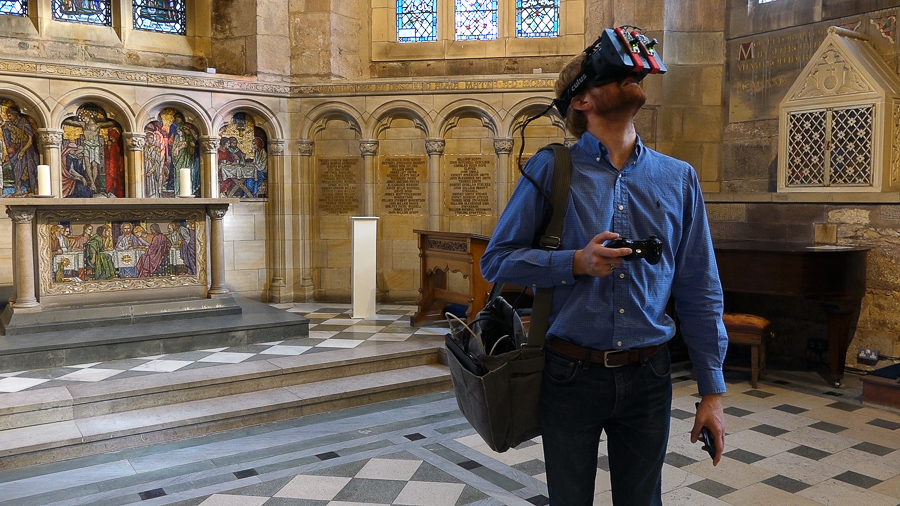
\includegraphics[width=\linewidth]{participant-m.jpg}
		\caption{Participant using Mirrorshades in user studies at St Salvator's chapel.}
		\label{participant-m.jpg}
	\end{center}
\end{figure}

%=========================================================================================================

\section{Evaluation Techniques}

As with the stage 1 investigation, a range of both qualitative and quantitative data were collected. Evaluating participants' preferences toward different styles of transitioning between RW and VR visual stimuli pertains to studying their reactions and responses to ascertain the effect upon their focus of attention, a concept that is largely psychological in nature and highly subjective~\cite{Ijsselsteijn2001}. Thus, subjective measures produced the bulk of the data for evaluation, however they are again backed up by objective log data to support or contradict any relationships that emerge.

Stage 2 participants completed the same pre-task questionnaire as the stage 1 participants and Likert-type questionnaires that shared certain items with that from stage 1 were also used; the stage 2.1 participants completed a 12-item questionnaire (included as appendix \ref{appendix-12-item-likert-type-questionnaire-stage-2-1}), while stage 2.2 participants completed a 9-item questionnaire (included as appendix \ref{appendix-9-item-likert-type-questionnaire-stage-2-2}). The SUS questionnaire was not used, while post-task interviews (prompts included as appendices \ref{appendix-interview-questions-stage-2-1} and \ref{appendix-interview-questions-stage-2-2} for stage 2.1 and stage 2.2 respectively) and logging were present. In addition to the Likert-type questionnaire, all stage 2 participants also completed the igroup presence questionnaire~\cite{Schubert2001} (IPQ, included as appendix \ref{appendix-igroup-presence-questionnaire}).

As presence does not have a single widely agreed upon definition and those definitions that are commonly used, including that adopted by this thesis of \textit{the experience of being in one place or environment, even when one is physically situated in another} (see section \ref{lit-review-presencec}), are subjective in nature due to the fact that presence (whether in physical or virtual environments) is perceptual~\cite{Waterworth2014}, attempts to quantify or `measure' the experience of presence are met with difficulty and many different approaches have been adopted, some more or less suitable to certain scenarios than others. Broadly, these approaches can be categorised as either subjective (most commonly post task questionnaires), behavioural (measurement/observation of actions that do not stem from conscious thought) or physiological (heart rate, skin conductance, etc.)~\cite{Insko2003}.

In this categorisation system, one could consider the log data recorded by the Mirrorshades platform to provide a behavioural insight into the participants' sense of presence and the interview and Likert-type questionnaires to provide a subjective insight. For this second stage of evaluation where direct comparison is made between different styles of transition in hopes of ascertaining which result in less pronounced breaks in presence (deflections upon the focus of attention axis of the combined Milgram/Waterworth model), the use of an established presence questionnaire was deemed a prudent addition to the evaluation techniques to inquire more directly about this aspect of the evaluation than the other evaluation techniques employed and in a standardised fashion.

%=========================================================================================================

\subsection{Presence Questionnaires}

Due to the nature of the Mirrorshades platform most established presence questionnaires could not be directly applied,  for they are predominantly written for application to `traditional' VR scenarios in which the user is immersed in a VR (or remote, in the case of telepresence) environment at the intentional exclusion of stimuli from their RW environment. Illustrated in reference to an embodied cognition framework, the sense of presence in such a scenario is argued to develop from the construction of a spatial-functional mental model of the VR environment, through a combination of representation of bodily actions as possible in the VR environment and suppression of incompatible sensory input from the RW environment~\cite{Schubert2001}. However considering a parallel reality scenario within the same framework, sensory input from a RW environment that features high spatial equivalence and a mutual vantage point with the VR environment is not incompatible; in fact it should be considered complimentary. Whereas a traditional VR experience attempts to create in the user's mind a new spatial-functional model that exists separate to, incompatible with and suppressing the model of their RW surroundings, parallel reality systems should instead be considered as enhancing the user's existing model of their RW surroundings, or alternatively as creating a complementary model that sits parallel to it and can be attended to in tandem.

This distinction is perhaps best explained as a difference in the use of the term `presence', \textit{``which is often used to refer to experiencing a purely VR as if it were a real place''}~\cite{Steed2014}, which can be visualised using the combined Milgram/Waterworth model. Established presence questionnaires largely assess presence in terms of the user's position upon the locus of attention axis, where `a sense of presence' means a position toward the VR extreme of the axis and `no sense of presence' means a position toward the RW extreme of the axis, with a break in presence considered under the original Slater and Steed definition (see discussion in section \ref{transitions_in_parallel_reality}) of a shift upon the locus of attention axis from VR to RW. In this stage of the evaluation into the Mirrorshades parallel reality platform however, the aim of the evaluation is to assess presence in terms of the user's position upon the focus of attention axis, to assess the severity of breaks in presence considered under the second of Waterworth and Waterworth's definitions (again, see discussion in section \ref{transitions_in_parallel_reality}) as deflections upon the focus of attention axis from the presence extreme in the direction of the absence extreme, representing increased cognitive load caused by performing a transition between two environments. Instead of assessing allocation of locus of attention between two \textit{incompatible} sets of environmental stimuli, this stage of evaluation hoped to assess the impact that a locus of attention oscillating between \textit{complimentary} sets of environmental stimuli has upon the participant's focus of attention. Instead of issuing a questionnaire designed to determine the balance between virtual presence and real presence, this investigation needed to issue a questionnaire to gain insight into the balance between presence (whether real or virtual) and absence.

Many established presence questionnaires that feature wording and weighting of questions associating negativity to awareness of the stimuli from the RW environment are thus unsuitable for use in assessment of a parallel reality scenario. Whilst this approach is ideal for a traditional VR scenario in which immersion in a VR environment at the complete exclusion of the user's RW environment is the ultimate goal, it does not apply well to a parallel reality scenario in which the ultimate goal is to imbue the user with the ability (\& desire) to freely transition between both RW and VR environments, wherein maintaining an awareness of one environment while perceiving stimuli from the other is likely beneficial, rather than detrimental, to the overall experience.

For example, Witmer and Singer's presence questionnaire~\cite{Witmer1998} poses several questions that directly enquire about aspects of the virtual environment (such as \textit{``13. How involved were you in the virtual environment experience?''}) but poses no questions that pertain to the RW environment other than a single comparison between VR and RW (\textit{``7. How much did your experiences in the virtual environment seem consistent with your real world experiences?''}, an assessment touching on perceived realism and of how well bodily actions were represented as possible in the VR environment). Other questionnaires, such as that used in an experiment by Slater and Steed in which participants walked through a VR field of trees~\cite{Slater1998}, are less extreme in their weighting toward questions only about VR, asking questions both directly about the VR environment (\textit{``Please rate your sense of being in the field among the plants''}) but also enquiring as to the sense of being in the RW environment with a neutral tone (\textit{``During the time of the experience, which was strongest on the whole, your sense of being in the virtual field, or of being in the real world of the laboratory?''}). However even this still permeates an `either or' implication to the two environments, emphasising their incompatibility and separateness.

%=========================================================================================================

\subsection{The Igroup Presence Questionnaire}
\label{igroup-presence-questionnaire-explanation}
The IPQ assesses presence based upon three factors; spatial presence (SP), involvement (INV) and realness (REAL). While SP questions assess how much bodily actions are represented as possible in the VR environment and REAL questions assess the `realness' of the VR environment by eliciting direct comparisons with the RW environment, INV questions assess suppression of incompatible sensory input from the RW environment but are not worded in a manner that presents attention paid to this sensory input as inherently negative (or even such that these stimuli are considered incompatible), reducing risk of negative bias when the questionnaire is applied to a scenario in which attention paid to RW stimuli is encouraged, such as an application of PR.

For a well implemented traditional VR experience that elicits a high sense of (virtual) presence in the user, one would expect their IPQ results to score highly in all three factors. As discussed by Constantin~\cite{Constantin2003a}, SP3 (\textit{``I did not feel present in the virtual space''}, anchored between \textit{``did not feel''} and \textit{``felt present''}) and INV2 (\textit{``I was not aware of my real environment''}, anchored between \textit{``fully disagree''} and \textit{``fully agree''}) would even seem to be fairly directly tied together, as a high involvement in the RW environment would intuitively reduce spatial presence by hampering the sense that bodily actions are possible in the VR environment.

However, in a parallel reality scenario that features high spatial equivalence between its constituent RW and VR environments, this tie between SP and INV may not demonstrate. Due to the spatial equivalence between the two environments and the fact that the user's view of the virtual is is of the equivalent vantage, bodily actions in the VR environment are inherently compatible with those in the RW environment (they could even be said to mimic or imitate them), so SP may score highly even when INV scores low, as RW sensory input isn't suppressed but in fact encouraged. In fact, it may even be the case that an inverse relationship presents between SP3 and INV2, as heightened awareness of the RW environment leads the user to a more believable representation of bodily actions in the VR environment as possible, increasing SP as (inherently possible) RW bodily actions are shared (`possible') with the VR environment.

Thus a conservative expectation for the results of the IPQ when applied to a parallel reality scenario would be for generally lower INV scores than a traditional VR scenario but without drastic reduction in SP scores. An optimistic expectation for a well implemented parallel reality scenario would be for lower INV scores and \textit{heightened} SP scores - that reinforcement of bodily actions within the RW environment will lead to an increase in experienced spatial presence in the VR environment.

Although a traditional view of augmented reality is that it aims to enhance the sense of presence in the physical world~\cite{Waterworth2014}, this does not necessarily stand as an aim of PR. This is due to the fact that instead of augmenting the primary environment of the user's RW surroundings parallel reality instead presents the user with two separate (debatably both or alternatingly `primary') environments.

%=========================================================================================================

%there isn't really a mapping from SP/INV/REAL to focus/locus/sensus.
% INV kinda maps to locus & effects focus

% ***but why didn't we add physiological measures as well?

%=========================================================================================================

\section{Stage 2.1 - Evaluating Transition styles}

Stage 2.1 followed a similar pattern to the stage 1 evaluation. Participants first received a `traditional' VR experience by using the DK1 and Xbox controller to explore the VR chapel while seated and subsequently completed the IPQ. This served both to acclimatize participants to the DK1 (in a similar vein as the use of the Tuscany demo in the stage 1 evaluation) and to produce baseline IPQ results for a traditional experience of the chapel model experienced via the DK1. Participants then performed two parallel reality scenarios in which they walked through the RW/VR chapels in a similar manner to the parallel reality scenario in stage 1 (see figure \ref{participant-m.jpg}), thus completing three scenarios in total;

\begin{enumerate}
	\item \textbf{Traditional VR scenario} - Participants explore the VR chapel from a stationary position, as VR has traditionally been employed at cultural heritage sites via CAVE installations and by the OVW group with Oculus HMDs, using the Xbox controller to move around the VR environment observed via the DK1, with the DK1 obscuring theier view of the RW chapel around them.
	\item \textbf{PR scenario with transitions 1-3} - Participants experience the RW and VR chapels in tandem using the Mirrorshades platform. They wear the DK1, holding the Xbox controller in their right hand and the smartphone in their left, with the laptop and control box bundle in a satchel worn over one shoulder. The default view on the DK1 screen is 100\% RW and participants are granted access to 3x different transition styles;
	\begin{enumerate}
		\item hard switch (see section \ref{sub-hardswitch}) mapped to controller \texttt{[A]} button (transition 1)
		\item transition with linear interpolation (see section \ref{transition-with-linear-interpolation}) mapped to controller \texttt{[B]} button (transition 2)
		\item analogue selectable opacity (see section \ref{analogue-selectable-opacity}) mapped to controller right trigger \texttt{[RT]} (transition 3)
\end{enumerate}
	\item \textbf{PR scenario with transitions 1-4} - Participants experience the same scenario as scenario 3, however this time with the introduction of the periodic hard switch (see section \ref{subsub-periodic}) which triggers a 0.15 second transition to 100\% VR every 3 seconds. The 3 second timer is reset each time the user manually triggers a transition using any one of transitions 1-3.
\end{enumerate}

In the parallel reality scenario with transitions 1-3 pressing and holding the \texttt{[A]} button triggered a hard switch from 100\% RW to 100\% VR, pressing and holding the \texttt{[B]} button triggered a linear interpolated switch from 100\% RW to 100\% VR and pulling on the right trigger \texttt{[RT]} reduced the opacity of the game objects upon which the camera feeds were rendered from 100\% to an amount that mapped to the amount that the trigger was pulled (pulling the trigger all the way in would reduce the opacity of the objects to 0\% and thus display 100\% VR, pulling the trigger 33\% would reduce the opacity of the objects by 33\% and thus display 66\% RW and 33\% VR, etc.). In the parallel reality scenario with transitions 1-4 participants were granted access to the same 3x transitions via the Xbox controller and additionally the 4th transition of the periodic hard switch was triggered every 3 seconds for a duration of 0.15 seconds. These two scenarios are referred to as `scenario 1-3' and `scenario 1-4' respectively in the following discussion.

Rather than describing a path through the chapel with particular positions of interest to stop and look around at, participants were simply told to slowly make their way from the starting position down to the altar end of the chapel. For at least one participant in the stage 1 evaluation, their exploration of the environments seemed to be subdued by their adherence to the prescribed route. In order to promote a more natural style of exploration the route description was thus not used in the second stage of evaluation.

%=========================================================================================================

\section{Stage 2.1 Results}

A total of 7 participants completed the stage 2.1 evaluation;
\begin{itemize}
	\item Age ranged from 18 to 27, with a mean of 22.3 and a standard deviation of 4
	\item 5x identified as male and 2x as female
	\item All reported previous experience with a games console controller
	\item None reported previous experience with a HMD
	\item 2x reported having previously visited the chapel
	\item None reported having previously experienced the virtual chapel
\end{itemize}

%=========================================================================================================

\begin{figure}[h]
	\begin{center}
	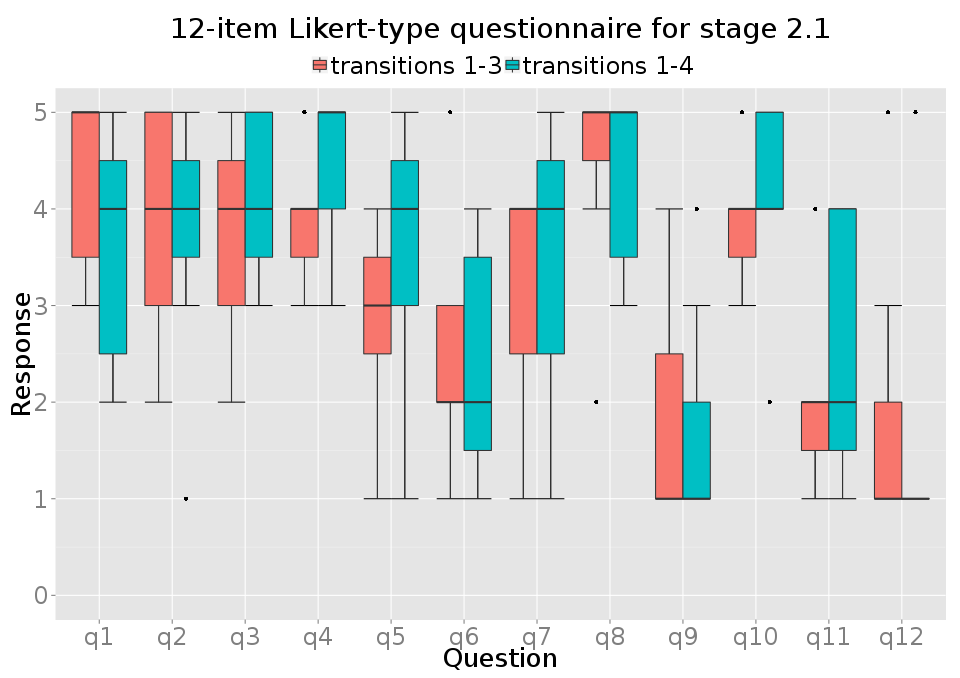
\includegraphics[width=.6\textwidth]{2.1/12-item-likert-type-questionnaire-boxplot.png}
	\caption{Stage 2.1 evaluation Likert-type questionnaire results.}
	\label{2-1-12-item-likert-type-questionnaire-boxplot.png}
	\end{center}
\end{figure}

%=========================================================================================================

\subsection{Likert-type Questionnaires}

When considering the responses to the Likert-type questionnaires (see figure \ref{2-1-12-item-likert-type-questionnaire-boxplot.png}) for the two parallel reality scenarios of the stage 2.1 evaluation, the following observations can be made.

\begin{itemize}
	\item Participants found the scenario 1-3 more enjoyable than scenario 1-4 (q1)
	\item Preference toward one transition style over others was in general less in scenario 1-3 than in scenario 1-4 (q2)
	\item Participants were more aware of both environments in scenario 1-4 than in scenario 1-3 (q3)
	\item Participants found it easier to compare features from past and present in scenario 1-4 than in scenario 1-3 (q4)
	\item Participants preferred to use one transition more than others in certain situations more in scenario 1-4 than they did in scenario 1-3 (q5), though responses varied widely
	\item Slightly more motion sickness was reported in scenario 1-4 (q7)
	\item Participants found scenario 1-3 to be a more rewarding way to explore the chapel (q8)
	\item Participants found that scenario 1-4 gave them a better understanding of what the chapel was like in the past (q10)
	\item Participants found switching between RW and VR more uncomfortable in scenario 1-4 than in scenario 1-3 (q11)
	\item Participants reported not noticing differences slightly more in scenario 1-3 than in scenario 1-4
\end{itemize}

%=========================================================================================================

\subsection{Interview Transcripts}

Once again, recordings of the structured interviews were transcribed after the chapel sessions and provided a wealth of qualitative insight into the participants' experiences with the Mirrorshades platform during the stage 2.1 evaluation.

Every single participant said that they preferred scenario 1-3 over scenario 1-4. In particular, one participant  reported that each time scenario 1-4 triggered an automatic transition (transition 4), s/he had to stop to regain their bearings, with another reporting that each transition 4 meant having to \textit{``stop and work it out again''}, a fairly direct description of how increased cognitive load caused by the switch overpowered the ability to process the (new) environmental stimuli - a break in presence. Several participants noted that they felt more \textit{``in control''} during scenario 1-3 than during scenario 1-4. Transition 4 was reported as being particularly off-putting when inaccuracy in the IPS had placed the virtual vantage at a position notably different to the participant's real position, especially when this resulted in virtual and real positions being on opposite sides of a wall.

Roughly half of the participants said that scenario 1-3 was more engaging, another found the scenarios roughly similar with regards to engagement and 2x found scenario 1-4 to be more engaging although they mentioned that they suspected this could simply have been down to increased familiarity with the system. Several participants said that transition 4 was \textit{``unexpected''}, leading to a less \textit{``consistent''} experience.

Responses were mixed when asked about whether one scenario allowed them to perceive more differences between RW and VR than the other. 3x participants reported experiencing no difference between the scenarios in this regard. 2x answered that they found scenario 1-3 better, one because the flash threw him/her off, the other because \textit{``you could fade between''}  although this feature (transition 3) was available in both scenarios. 2x chose 1-4 as better, one because transition 4 would happen when s/he wasn't prepared for a transition and thus s/he would \textit{``notice that something had moved, whereas if I knew I was switching I would maybe subconsciously expecting things to move''}, an observation that likens to the `sudden discovery' aspect of Briand's Hagia Eirene piece (see section \ref{the-mirrorshades-platform}).

All but one participant reported preferring transition 3 accessed via the right trigger \texttt{[RT]} to the other transitions. The one participant who answered otherwise elaborated that they did not notice much difference between the different transition styles and when thinking back to the scenarios was \textit{``not sure which one I was using now!''}. Looking at the log data for this participant however (see section \ref{2-1-log-data}) they did nonetheless make use of all the transition styles in both scenarios 1-3 and 1-4, heavily favouring the hard switch transition 1 in scenario 1-4. When asked why they preferred transition 3, participants reported liking how being able to control the opacity allowed them to \textit{``see elements of both''} environments at once, to \textit{``simultaneously measure the historical differences''}, with the trigger giving them more \textit{``control''}.

Responses when asked about motion sickness varied greatly. One participant reported none at all in either scenario, while one reported some motion sickness when seated and using the analogue stick of the Xbox controller to turn their virtual presence and also when walking in the parallel reality scenario when the IPS was inaccurate. One participant reported motion sickness that increased with time, being comfortable for the first 2/3rds of each scenario and with both parallel reality scenarios being worse than the traditional seated scenario. Three participants reported motion sickness only when walking in the parallel reality scenarios; of these, one reported that it was worse in scenario 1-4 and another said that motion sickness only occurred when looking at RW via the cameras. One participant only experienced motion sickness after removing the DK1.

Other comments included not knowing where they were in the chapel inducing motion sickness and that accuracy of the IPS needed improvement, with sudden large VR movements inducing motion sickness. Furthermore, one participant commented directly upon the relationship between `immersion' and perceived realism of the VR environment - \textit{``\ldots obviously it wasn't the same quality, but I still felt so immersed in it. Even though part of me would've known it wasn't real, most of it felt real even though it didn't look like it''}.

%=========================================================================================================

\subsection{Log Data}
\label{2-1-log-data}

Log data were recorded during all scenarios, however these data were not recorded for 4 out of the 7 participants for the traditional seated scenario thus detailed comparisons cannot reasonably be made between the traditional VR scenario and the parallel reality scenarios. Log data were however successfully recorded for both parallel reality scenarios and as such comparisons can be made between the parallel reality scenarios and within each parallel reality scenarios, which was the aim of this stage of the evaluation.

%=====================

\subsubsection{Considering all scenarios (traditional and PR)}

For all participants there was once again substantially more yaw change than pitch change, in both traditional and parallel reality scenarios. Figure \ref{2-1-8-pitch-yaw-trad-1-3-1-4.png} shows this relationship by plotting pitch and yaw against time for participant 8 for all three scenarios (traditional at left, scenario 1-3 in the middle and scenario 1-4 at right) and the standard deviations for pitch and yaw for all participants across all three scenarios is given by tables \ref{2-1-sd-trad}, \ref{2-1-sd-1-3} and \ref{2-1-sd-1-4}.

\begin{figure}[h]
	\begin{center}
	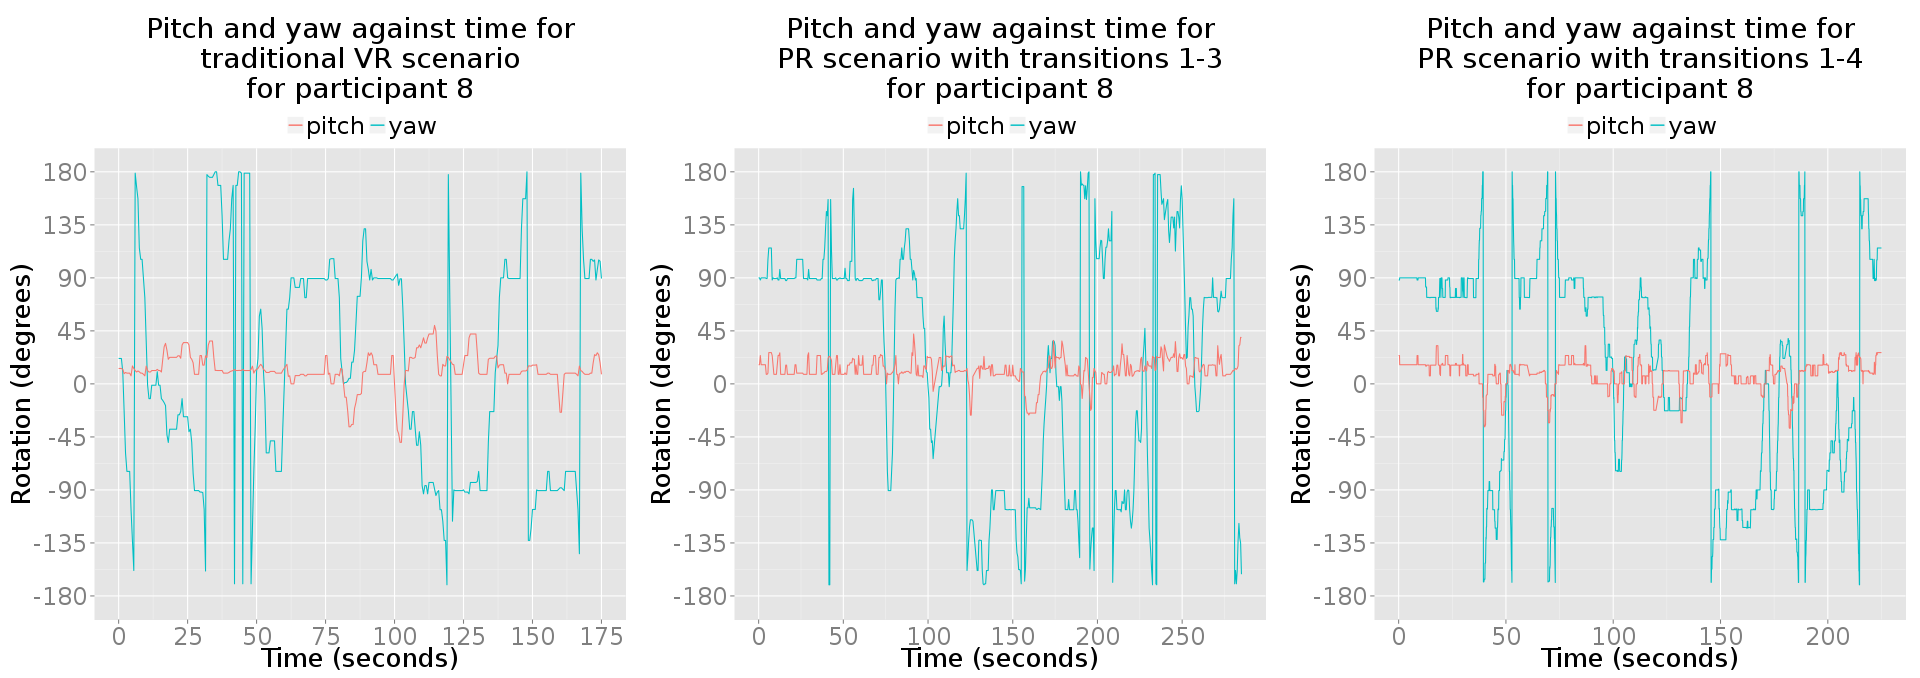
\includegraphics[width=\textwidth]{2.1/8-pitch-yaw-trad-1-3-1-4.png}
	\caption{Pitch and yaw against time for participant 8 in traditional and both parallel reality scenarios.}
	\label{2-1-8-pitch-yaw-trad-1-3-1-4.png}
	\end{center}
\end{figure}

\begin{table}
\begin{center}
\begin{minipage}[t]{.45\linewidth}
\begin{center}
\begin{tabularx}{\textwidth}{c *{3}{>{\centering\arraybackslash}X}}
\toprule

\textbf{Participant} & \textbf{Pitch (\textdegree)} & \textbf{Yaw (\textdegree)} \\

\midrule

7 & 13.013 & 87.822 \\

8 & 13.917 & 94.436 \\

9 & 12.039 & 87.956 \\

10 & no data & no data \\

11 & no data & no data \\

12 & no data & no data \\

13 & no data & no data \\

\bottomrule
\end{tabularx}
\caption{Standard deviation in pitch and yaw for traditional VR scenario.}
\label{2-1-sd-trad}
\end{center}
\end{minipage}
\end{center}
\end{table}

\begin{table}
\begin{center}
\begin{minipage}[t]{.45\linewidth}
\begin{center}
\begin{tabularx}{\textwidth}{c *{3}{>{\centering\arraybackslash}X}}
\toprule

\textbf{Participant} & \textbf{Pitch (\textdegree)} & \textbf{Yaw (\textdegree)} \\

\midrule

7 & no data & no data \\

8 & 10.253 & 102.254 \\

9 & 13.734 & 84.076 \\

10 & 17.833 & 84.578 \\

11 & 11.540 & 76.445 \\

12 & 19.635 & 74.696 \\

13 & 22.095 & 91.827 \\

\bottomrule
\end{tabularx}
\caption{Standard deviation in pitch and yaw for parallel reality scenario with transitions 1-3 (RW and VR periods combined).}
\label{2-1-sd-1-3}
\end{center}
\end{minipage}
%
\begin{minipage}[t]{.02\linewidth}
\hfill%
\end{minipage}
%
\begin{minipage}[t]{.45\linewidth}
\begin{center}
\begin{tabularx}{\textwidth}{c *{3}{>{\centering\arraybackslash}X}}
\toprule

\textbf{Participant} & \textbf{Pitch (\textdegree)} & \textbf{Yaw (\textdegree)} \\

\midrule

7 & no data & no data \\

8 & 11.493 & 89.531 \\

9 & 12.365 & 95.144 \\

10 & 14.059 & 90.429 \\

11 & 8.354 & 82.279 \\

12 & 22.202 & 75.425 \\

13 & 19.530 & 62.321 \\

\bottomrule
\end{tabularx}
\caption{Standard deviation in pitch and yaw for parallel reality scenario with transitions 1-4 (RW and VR periods combined).}
\label{2-1-sd-1-4}
\end{center}
\end{minipage}
\end{center}
\end{table}

%=====================

\subsubsection{Comparing RW and VR periods within parallel reality scenarios}

When comparing pitch and yaw data between the RW and VR periods within the two parallel reality scenarios, five out of the seven participants displayed greater variance in yaw when perceiving VR stimuli than when perceiving RW stimuli for both scenario 1-3 and scenario 1-4. Figure \ref{8-1-3-pitch-yaw.png} illustrates this relationship for participant 8 undertaking scenario 1-3 while figure \ref{12-1-4-pitch-yaw.png} illustrates the relationship for participant 12 undertaking scenario 1-4. Again the background colouring of the plots represents whether the participant was perceiving RW or VR visual stimuli at a particular time index, using different colours to indicate which transition style was used to view the VR stimuli; pink for transition 1, green for transition 2, yellow for transition 3 and dark blue for transition 4.

\begin{figure}[h]
	\begin{center}
	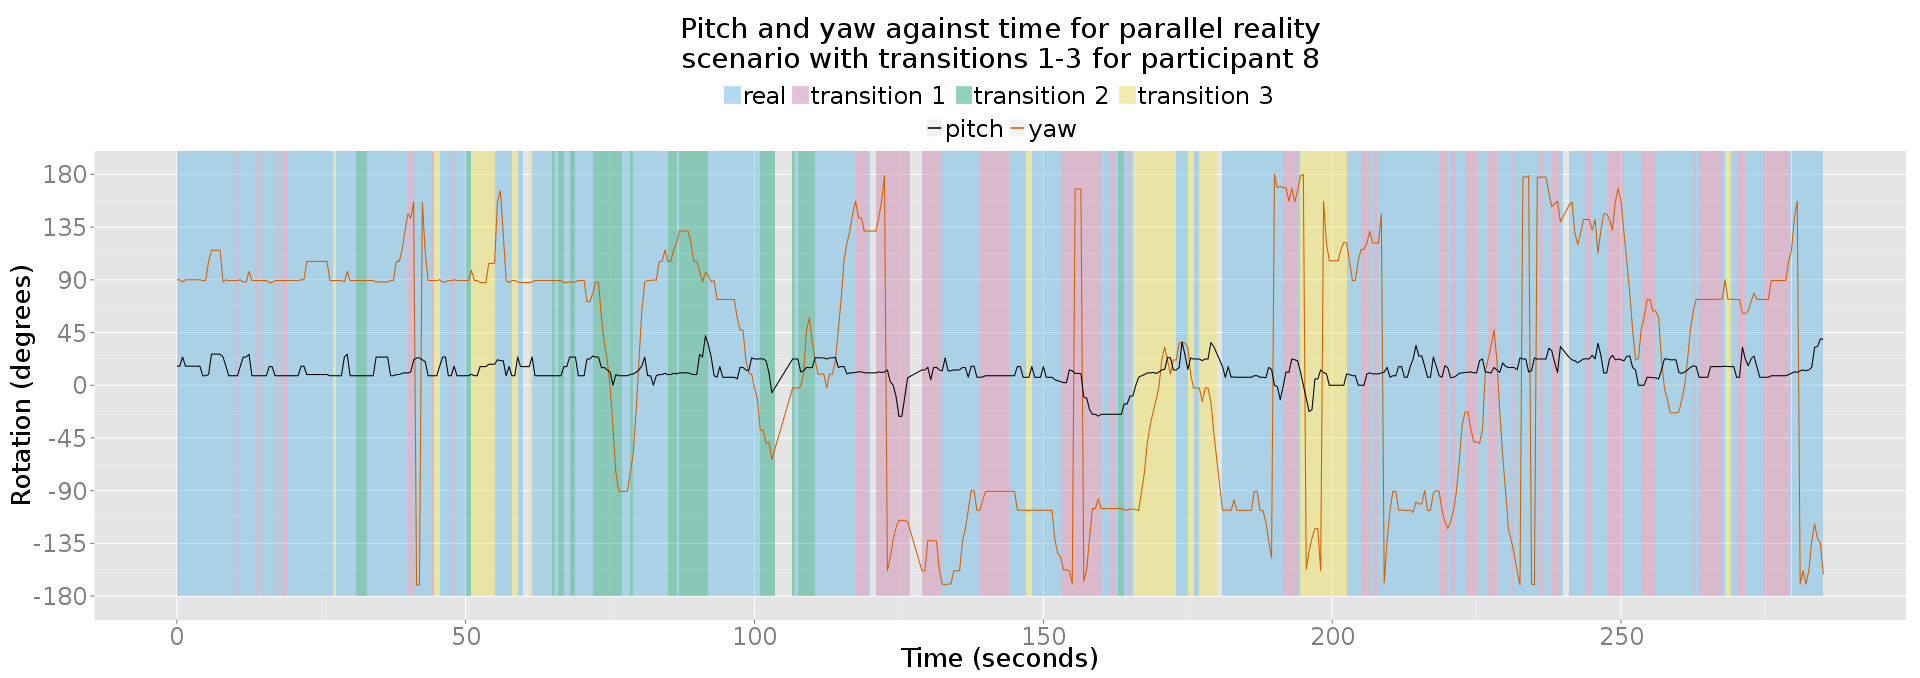
\includegraphics[width=\textwidth]{2.1/8-1-3-pitch-yaw.png}
	\caption{Pitch and yaw against time for participant 8 in scenario 1-3, showing RW/VR transitions.}
	\label{8-1-3-pitch-yaw.png}
	\end{center}
\end{figure}

%\begin{figure}[h]
%	\begin{center}
%	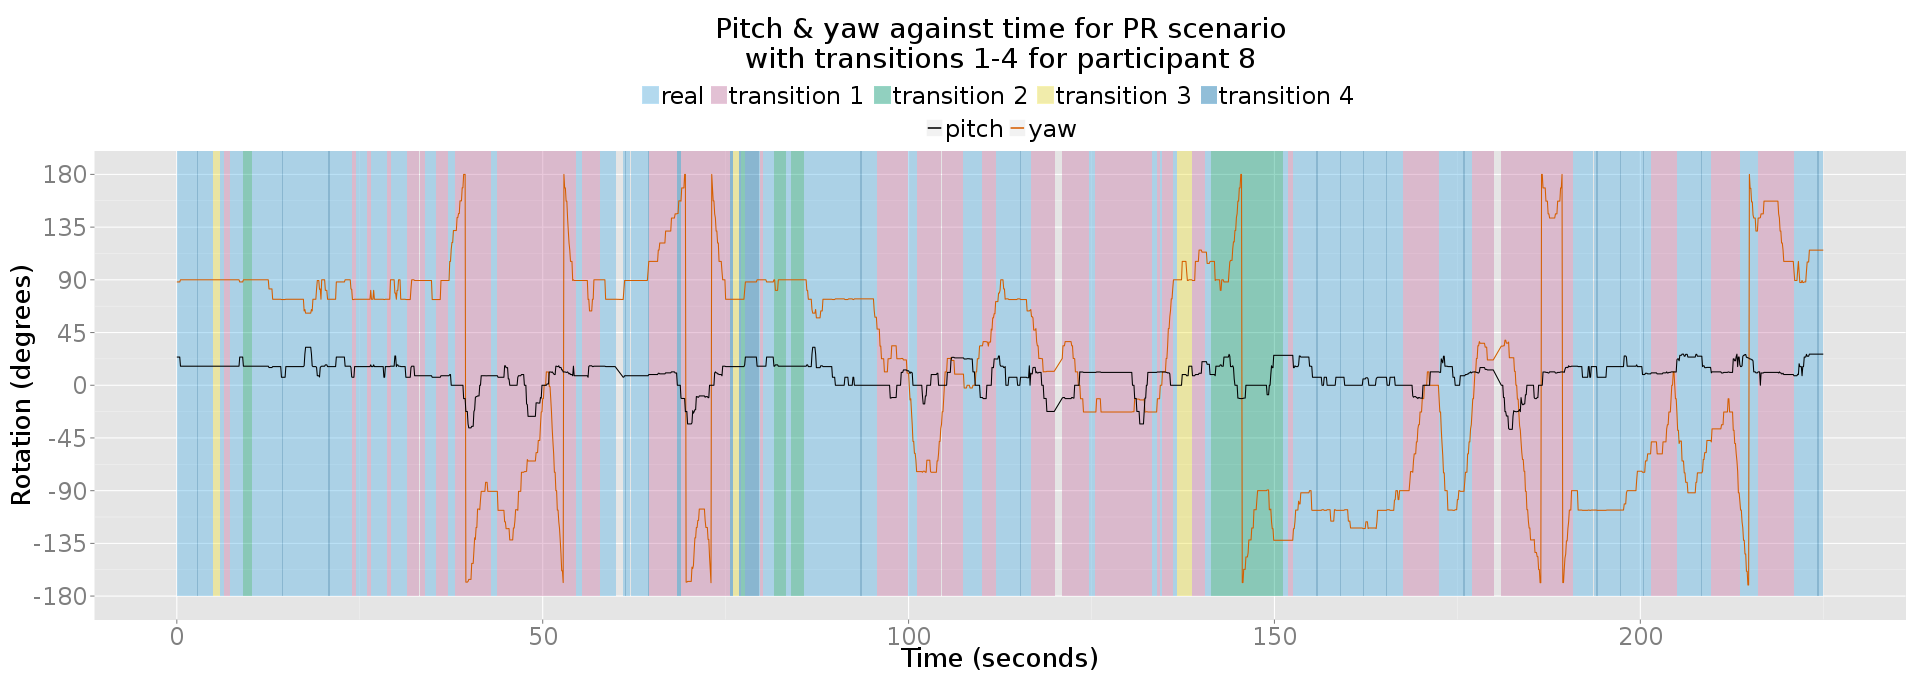
\includegraphics[width=\textwidth]{2.1/8-1-4-pitch-yaw.png}
%	\caption{Pitch and yaw against time for participant 8 in scenario 1-4, showing RW/VR transitions.}
%	\label{8-1-4-pitch-yaw.png}
%	\end{center}
%\end{figure}

\begin{figure}[h]
	\begin{center}
	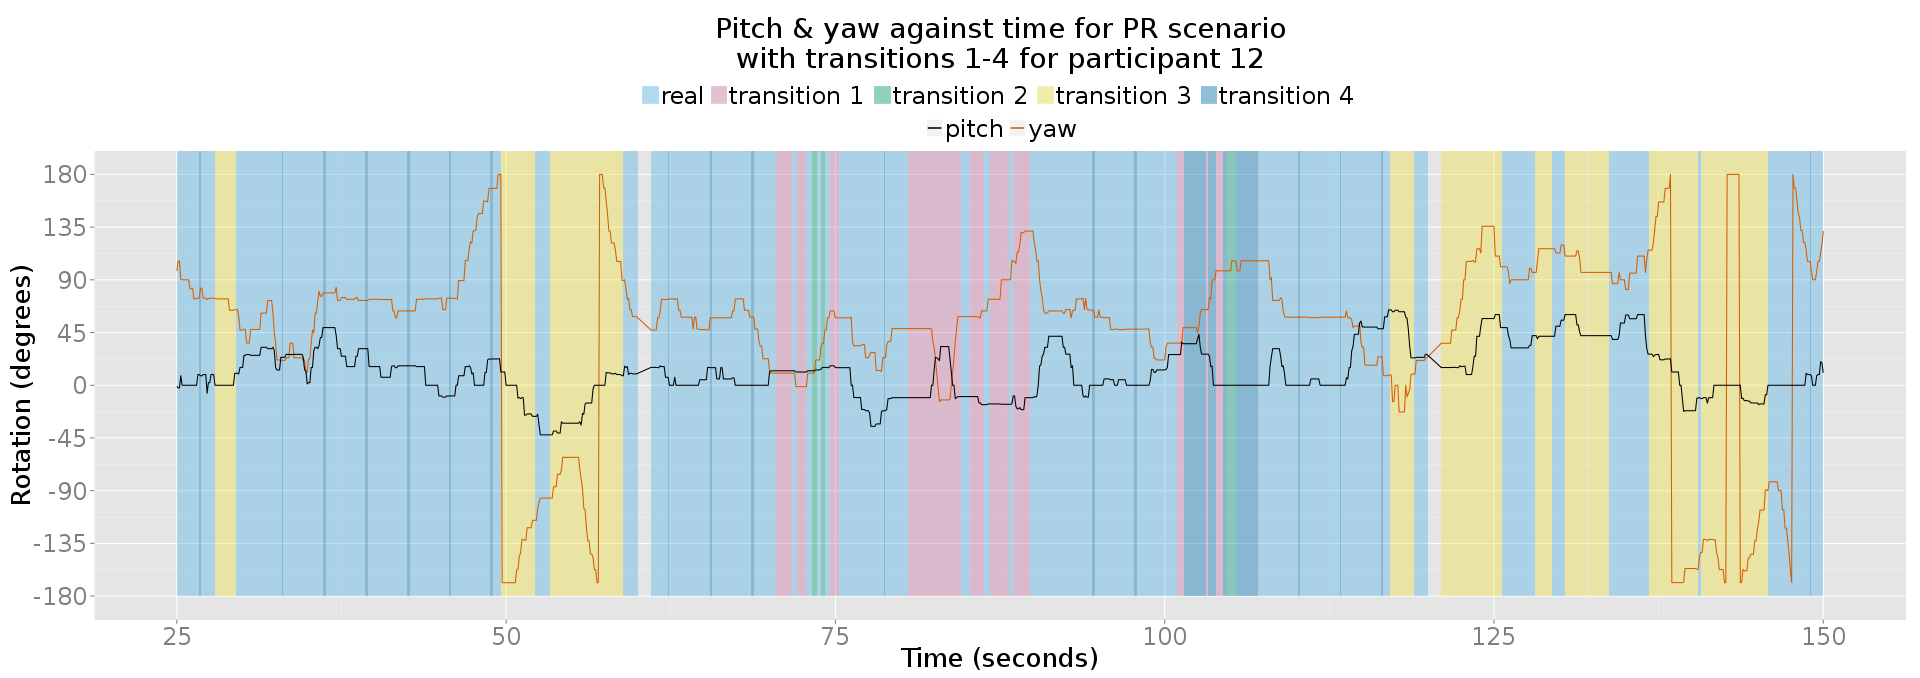
\includegraphics[width=\textwidth]{2.1/12-1-4-pitch-yaw.png}
	\caption{Pitch and yaw against time for participant 12 in scenario 1-4, showing RW/VR transitions.}
	\label{12-1-4-pitch-yaw.png}
	\end{center}
\end{figure}

When comparing head movement as mean standard deviation weighted by duration of the periods (tables \ref{mean-sd-yaw-1-3} and \ref{mean-sd-yaw-1-4}) between the RW and VR portions of the two parallel reality scenarios, this relationship is seen much more substantially in scenario 1-4. Part of this is due to the fact that all participants in scenario 1-4 showed less change in yaw in the RW periods than in the RW periods of scenario 1-3. Whilst this apparent increased comfort with larger head movements in VR in scenario 1-4 could be explained due to familiarity, the magnitude of the difference between scenario 1-3 and scenario 1-4 makes it hard to believe that familiarity is the sole reason, especially considering that scenario 1-4 was not a drastically different experience to scenario 1-3 as only the addition of transition 4 differentiated it from scenario 1-3. One possible contributor, as mentioned by one participant during the interview stage, is that they spent more time perceiving VR in order to avoid the automatic transition that would occur when perceiving RW.

\begin{table}
\begin{center}
\begin{minipage}[t]{.45\linewidth}
\begin{center}
\begin{tabularx}{\textwidth}{c *{3}{>{\centering\arraybackslash}X}}
\toprule

\textbf{Participant} & \textbf{RW (\textdegree)} & \textbf{VR (\textdegree)} \\

\midrule

7 & no data & no data \\

8 & 41.680 & 42.228 \\

9 & 19.274 & 31.133 \\

10 & 13.541 & 16.758 \\

11 & 28.030 & 16.751 \\

12 & 38.654 & 28.494 \\

13 & 29.623 & 39.717 \\

\bottomrule
\end{tabularx}
\caption{Weighted mean sd in yaw for scenario 1-3.}
\label{mean-sd-yaw-1-3}
\end{center}
\end{minipage}
%
\begin{minipage}[t]{.02\linewidth}
\hfill%
\end{minipage}
%
\begin{minipage}[t]{.45\linewidth}
\begin{center}
\begin{tabularx}{\textwidth}{c *{3}{>{\centering\arraybackslash}X}}
\toprule

\textbf{Participant} & \textbf{RW (\textdegree)} & \textbf{VR (\textdegree)} \\

\midrule

7 & 20.228 & 50.963 \\

8 & 10.783 & 50.593 \\

9 & 13.579 & 27.398 \\

10 & 10.7334 & 34.981 \\

11 & 13.500 & 13.513 \\

12 & 16.248 & 50.326 \\

13 & 7.269 & 57.162 \\

\bottomrule
\end{tabularx}
\caption{Weighted mean sd in yaw for scenario 1-4.}
\label{mean-sd-yaw-1-4}
\end{center}
\end{minipage}
\end{center}
\end{table}

%=====================

\subsubsection{Experimenting With Transition Styles}

Some participants showed an understandable behaviour where they `tried out' the different transition styles before adopting one that they then used predominantly throughout the rest of the scenario. Participant 11 showed this behaviour in its most extreme case during scenario 1-3, when s/he tried each transition style just once at the very beginning of the scenario and then only used transition 3 (via the right trigger \texttt{[RT]}) throughout the rest of the scenario (figure \ref{11-pitch-yaw-1-3.png}). However when s/he came to perform scenario 1-4, s/he seemed to take this opportunity as a second chance to experiment with all of the different transition styles, using transitions 1, 2 and 3 at different points throughout the scenario (figure \ref{11-pitch-yaw-1-4.png}).

\begin{figure}[h]
	\begin{center}
	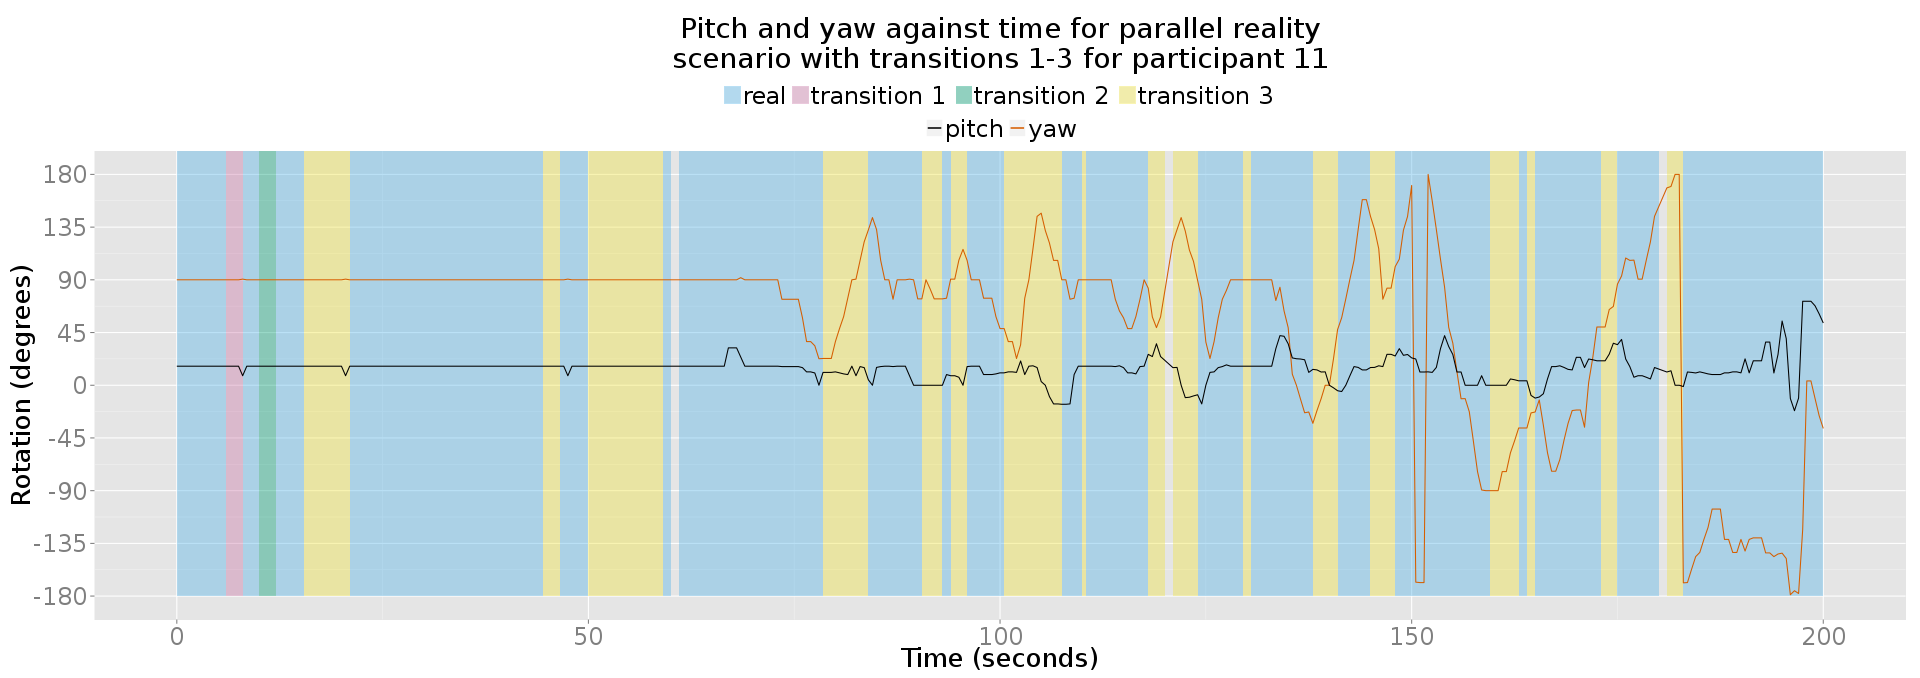
\includegraphics[width=\textwidth]{2.1/11-pitch-yaw-1-3.png}
	\caption{Pitch and yaw against time for participant 11 in scenario 1-3, showing RW/VR transitions.}
	\label{11-pitch-yaw-1-3.png}
	\end{center}
\end{figure}

\begin{figure}[h]
	\begin{center}
	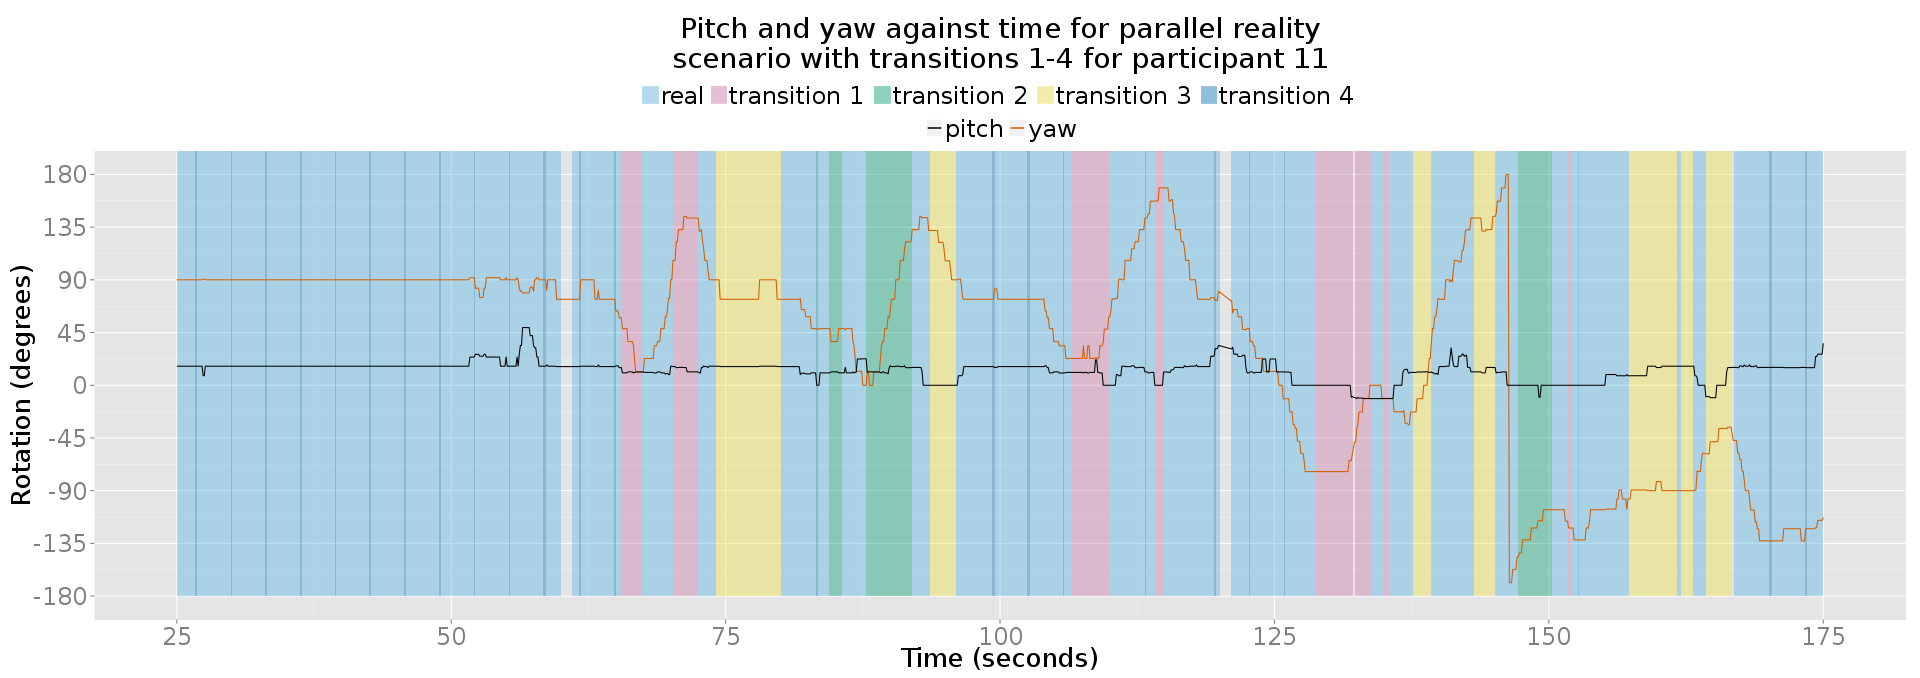
\includegraphics[width=\textwidth]{2.1/11-pitch-yaw-1-4.png}
	\caption{Pitch and yaw against time for participant 11 in scenario 1-3, showing RW/VR transitions.}
	\label{11-pitch-yaw-1-4.png}
	\end{center}
\end{figure}

Participant 7 showed this behaviour in a less extreme fashion, spending more time with each of the three user-controllable transition styles before settling upon transition 3, during scenario 1-4 (figure \ref{7-pitch-yaw-1-4.png}).

\begin{figure}[h]
	\begin{center}
	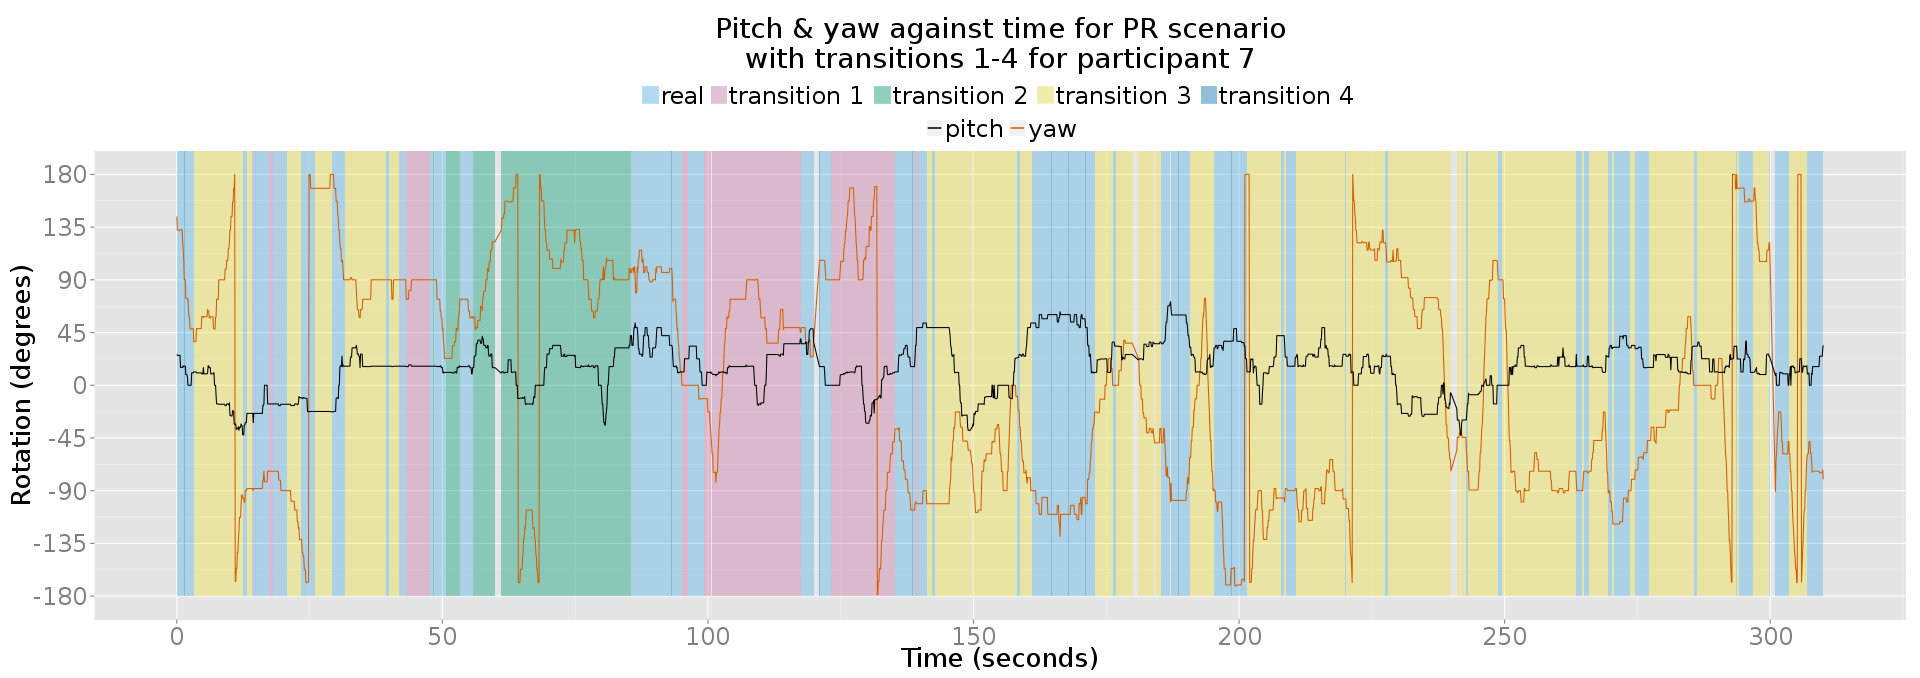
\includegraphics[width=\textwidth]{2.1/7-pitch-yaw-1-4.png}
	\caption{Pitch and yaw against time for participant 7 in scenario 1-4, showing RW/VR transitions.}
	\label{7-pitch-yaw-1-4.png}
	\end{center}
\end{figure}

Some participants however continued to use all available transition styles throughout a session, such as participant 13 during scenario 1-3 (figure \ref{13-pitch-yaw-1-3.png}). This was one of the longest individual sessions, with the participant exploring the RW and VR chapels in tandem in parallel reality via the Mirrorshades platform for over 8.5 minutes. During the interview, s/he reported preferring transition 3 via the right trigger \texttt{[RT]} which is corroborated by the data - s/he triggered this transition more than transition 1 or 2 (25 times total, compared to 20 for transition 1 and 14 for transition 2) and spent longer perceiving VR via transition 3 (103 seconds total compared to 81.5 seconds for transition 1 and 20 seconds for transition 2, with a mean of 4.12 seconds for each period using transition 3, 4.075 seconds for transition 1 and 1.429 seconds for transition 2).

\begin{figure}[h]
	\begin{center}
	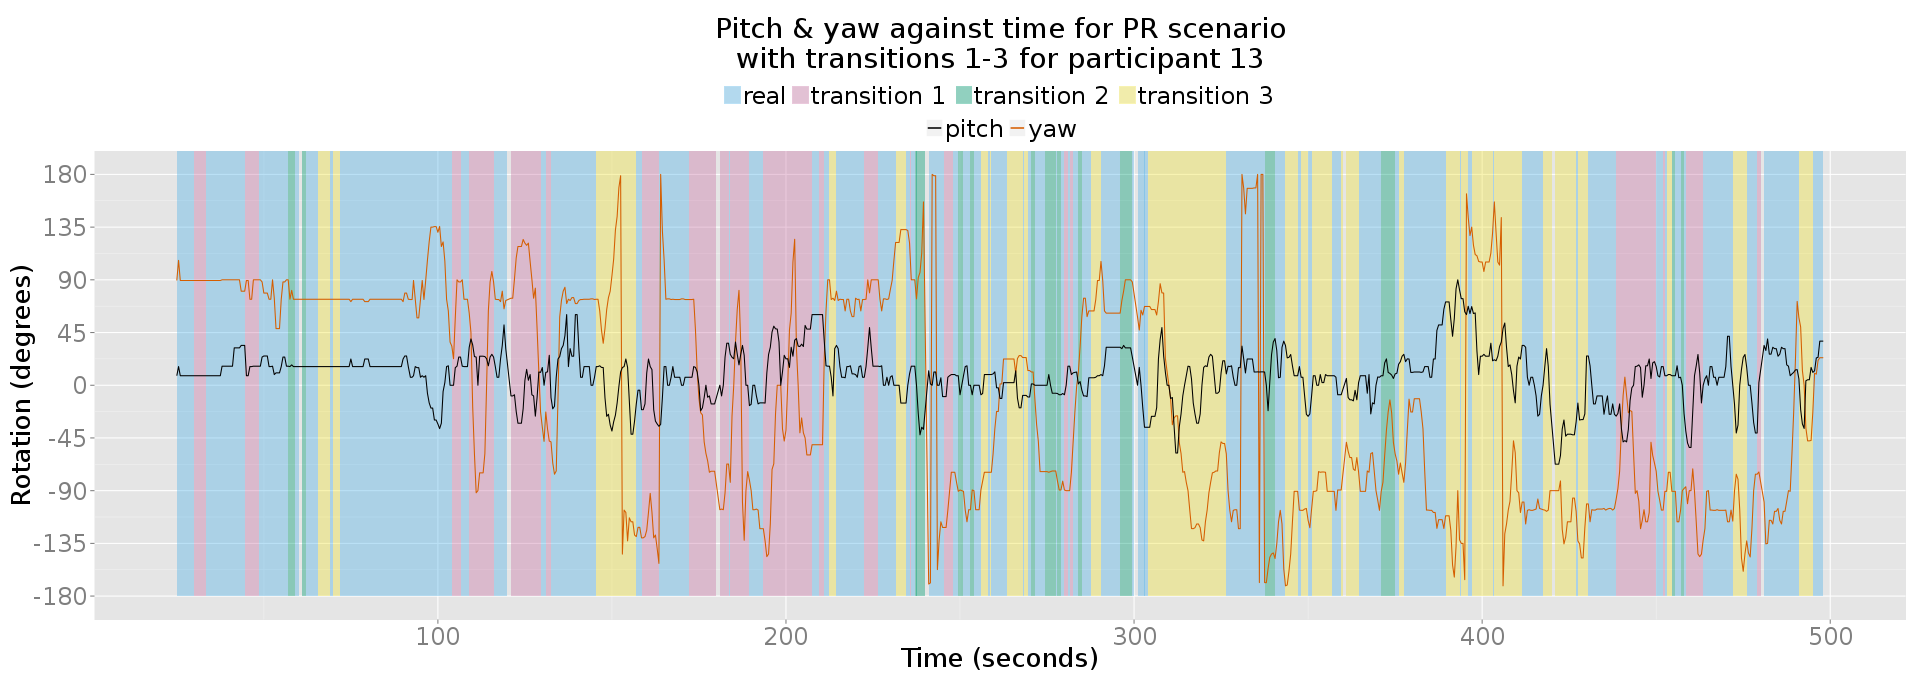
\includegraphics[width=\textwidth]{2.1/13-pitch-yaw-1-3.png}
	\caption{Pitch and yaw against time for participant 13 in scenario 1-3, showing RW/VR transitions.}
	\label{13-pitch-yaw-1-3.png}
	\end{center}
\end{figure}

%=====================

\subsubsection{Walking and Head Movement}

As seen in the results to the stage 1 evaluation, there is also a correlation in the stage 2.1 results between position and change in head movement, with several participants displaying greater variance in head pitch and yaw while standing still than when walking with the DK1. This is true for both parallel reality scenarios; figure \ref{8-1-3_2up.png} shows pitch and yaw against time above, aligned with distance moved against time below, for participant 8 performing scenario 1-3, while figure \ref{9-1-4_2up.png} shows the same arrangement for participant 9 performing scenario 1-4. Especially after taking into consideration the slight lag in IPS data, the stationary periods starting around 120, 160, 200 and 240 seconds in figure \ref{8-1-3_2up.png} and those starting around 70, 150 and 210 seconds in figure \ref{9-1-4_2up.png} all closely coincide with pronounced variance in yaw.

\begin{figure}[h]
	\begin{center}
	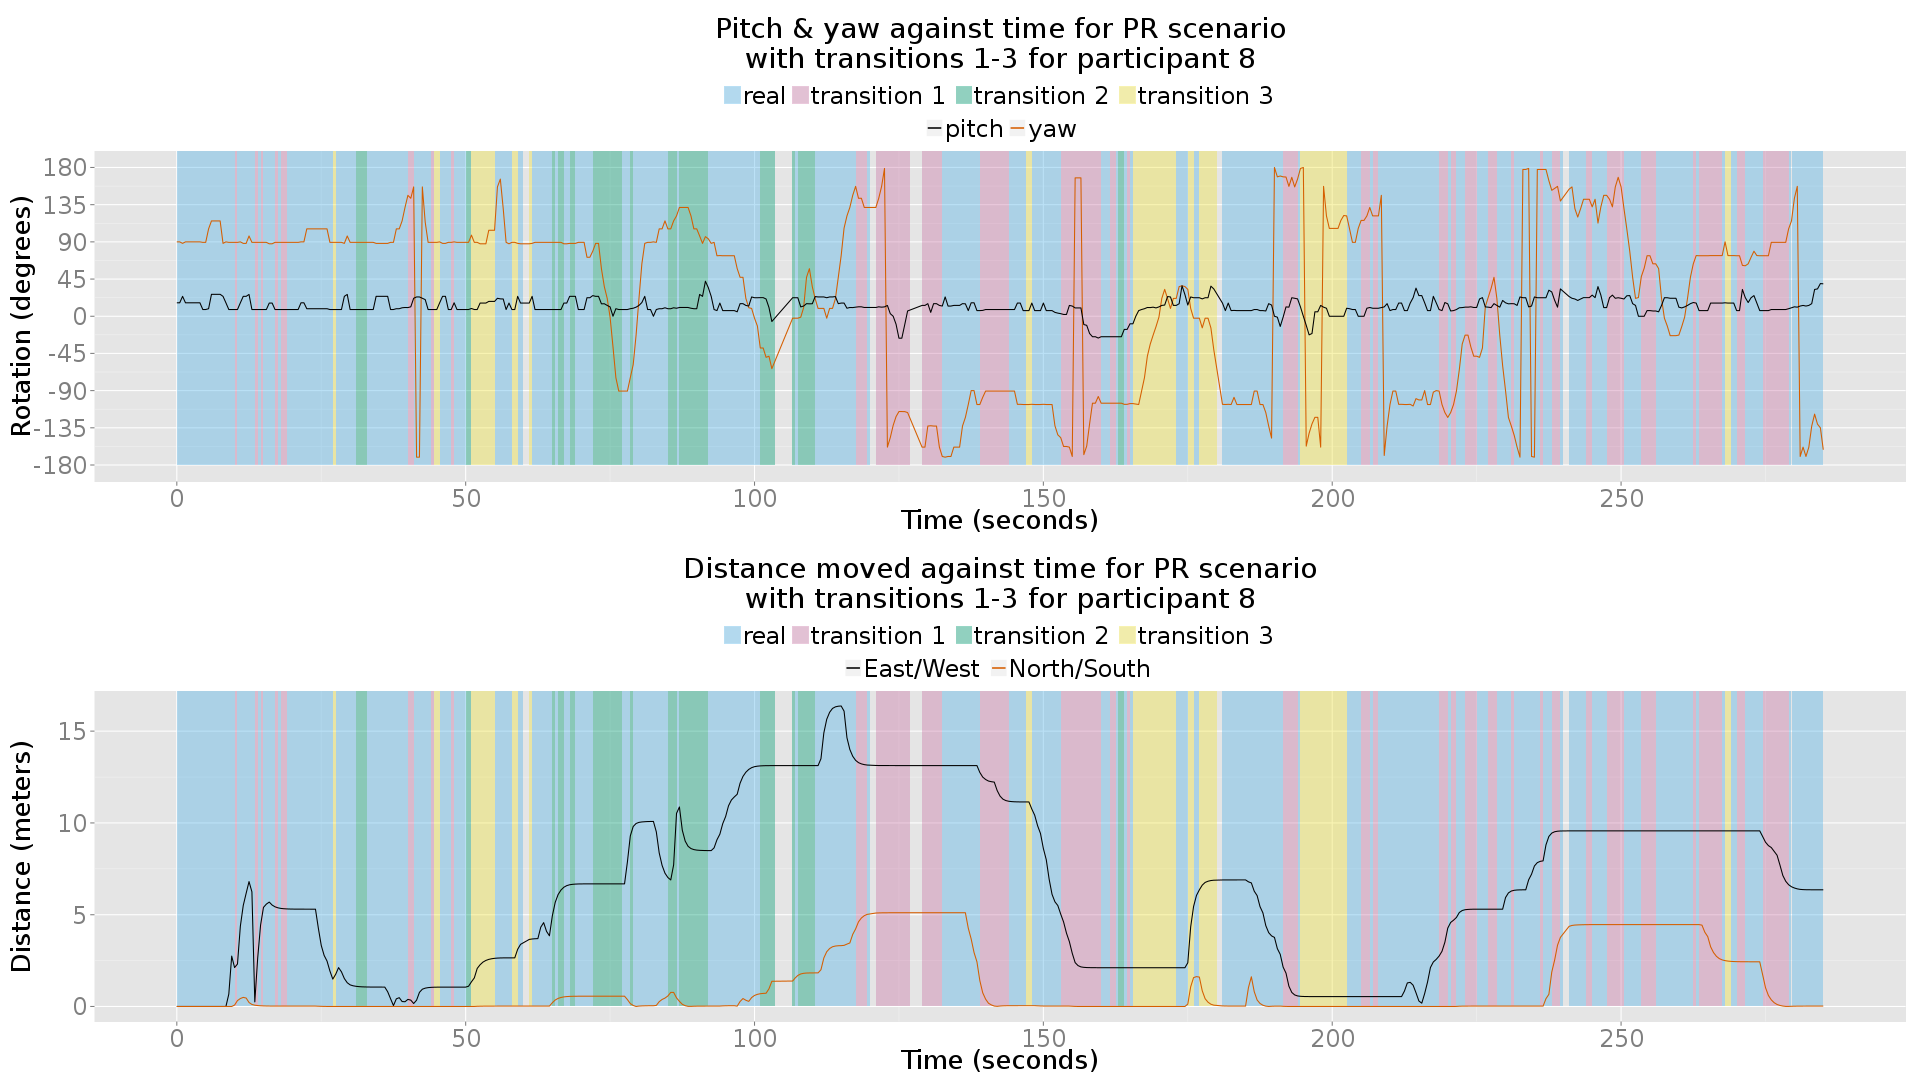
\includegraphics[width=\textwidth]{2.1/8-1-3_2up.png}
	\caption{Pitch and yaw against time aligned with distance moved against time for participant 8 in scenario 1-3, showing RW/VR transitions.}
	\label{8-1-3_2up.png}
	\end{center}
\end{figure}

\begin{figure}[h]
	\begin{center}
	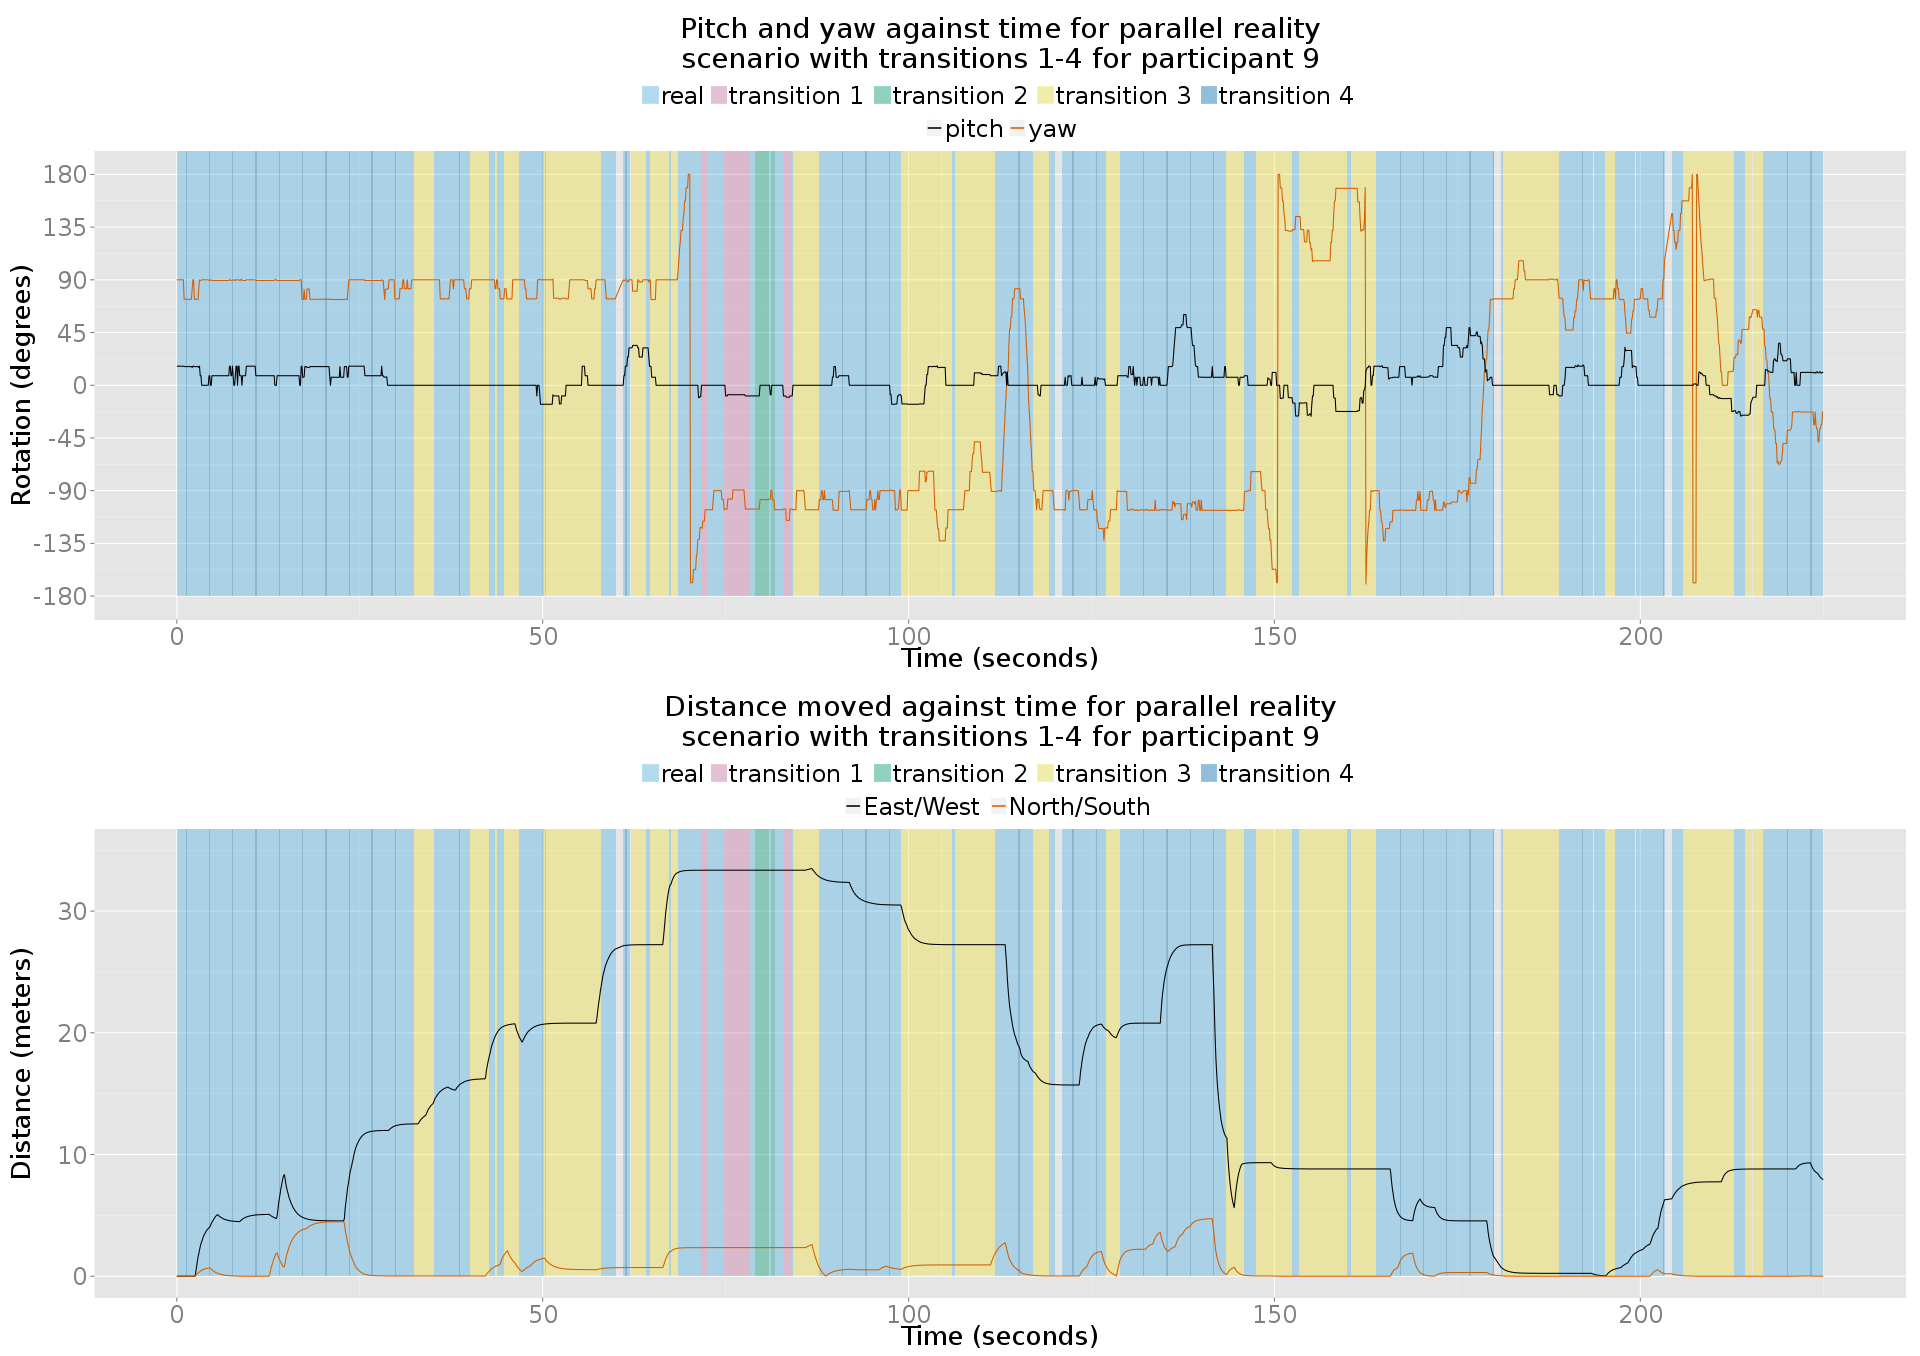
\includegraphics[width=\textwidth]{2.1/9-1-4_2up.png}
	\caption{Pitch and yaw against time aligned with distance moved against time for participant 9 in scenario 1-4, showing RW/VR transitions.}
	\label{9-1-4_2up.png}
	\end{center}
\end{figure}

%=====================

\subsubsection{Use of Intermediary Opacities}

Confirming responses during the post task interviews, several participants did make use of the analogue selectable transition (transition 3, accessed via the right trigger \texttt{[RT]}) to view both RW and VR environments together. Figures \ref{10-1-4_opacity.png} and \ref{12-1-4_opacity.png} show, for participants 10 and 12 respectively undertaking scenario 1-4, the opacity of the objects upon which the camera feeds were rendered: an opacity of 1.0 means that the camera feed was completely opaque and the participant was thus perceiving 100\% RW visual stimuli, while an opacity of 0 means that the camera feed was invisible and the participant was perceiving 100\% VR visual stimuli. As well as using the analogue selectable transition to view both environments at once, there are incidents where it seems that the participant used the analogue selectable opacity not strictly to view both environments at once, but to control the speed at which a transition from RW to VR was performed. We can see that participant 10 (figure \ref{10-1-4_opacity.png}) uses transition 3 at around 250 seconds to perform a transition to a 100\% VR view, but at a slower rate than the linear interpolated transition such as can be seen just before at around 245 seconds. This greater level of control in how quickly transitions were performed was raised in interviews as a reason why this particular transition was favoured by some participants.

\begin{figure}[h]
	\begin{center}
	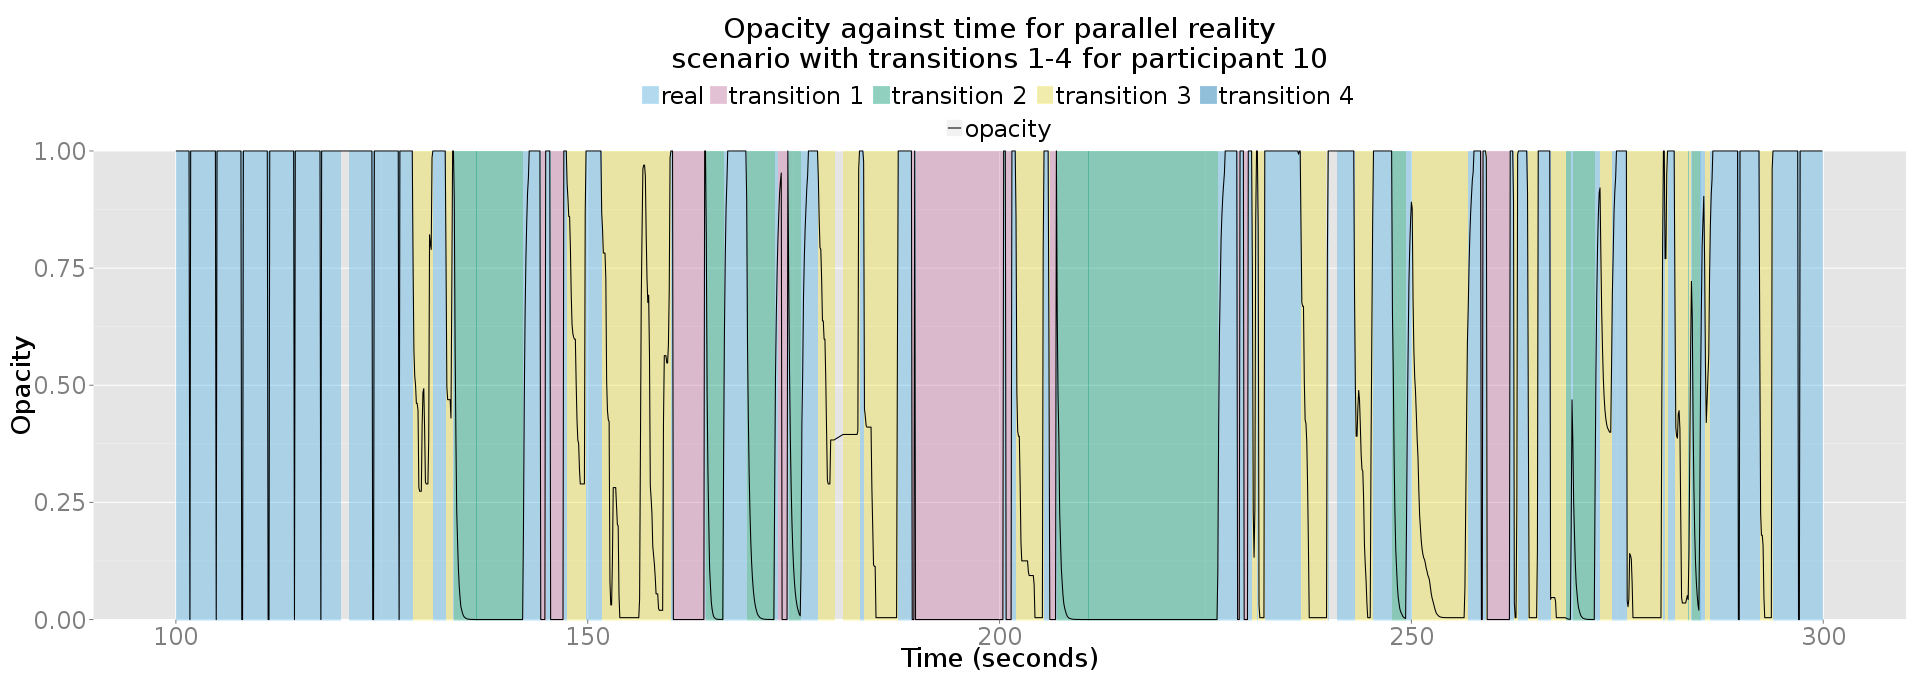
\includegraphics[width=\textwidth]{2.1/10-1-4_opacity.png}
	\caption{Opacity of camera objects against time for participant 10 in scenario 1-4, showing RW/VR transitions.}
	\label{10-1-4_opacity.png}
	\end{center}
\end{figure}

\begin{figure}[h]
	\begin{center}
	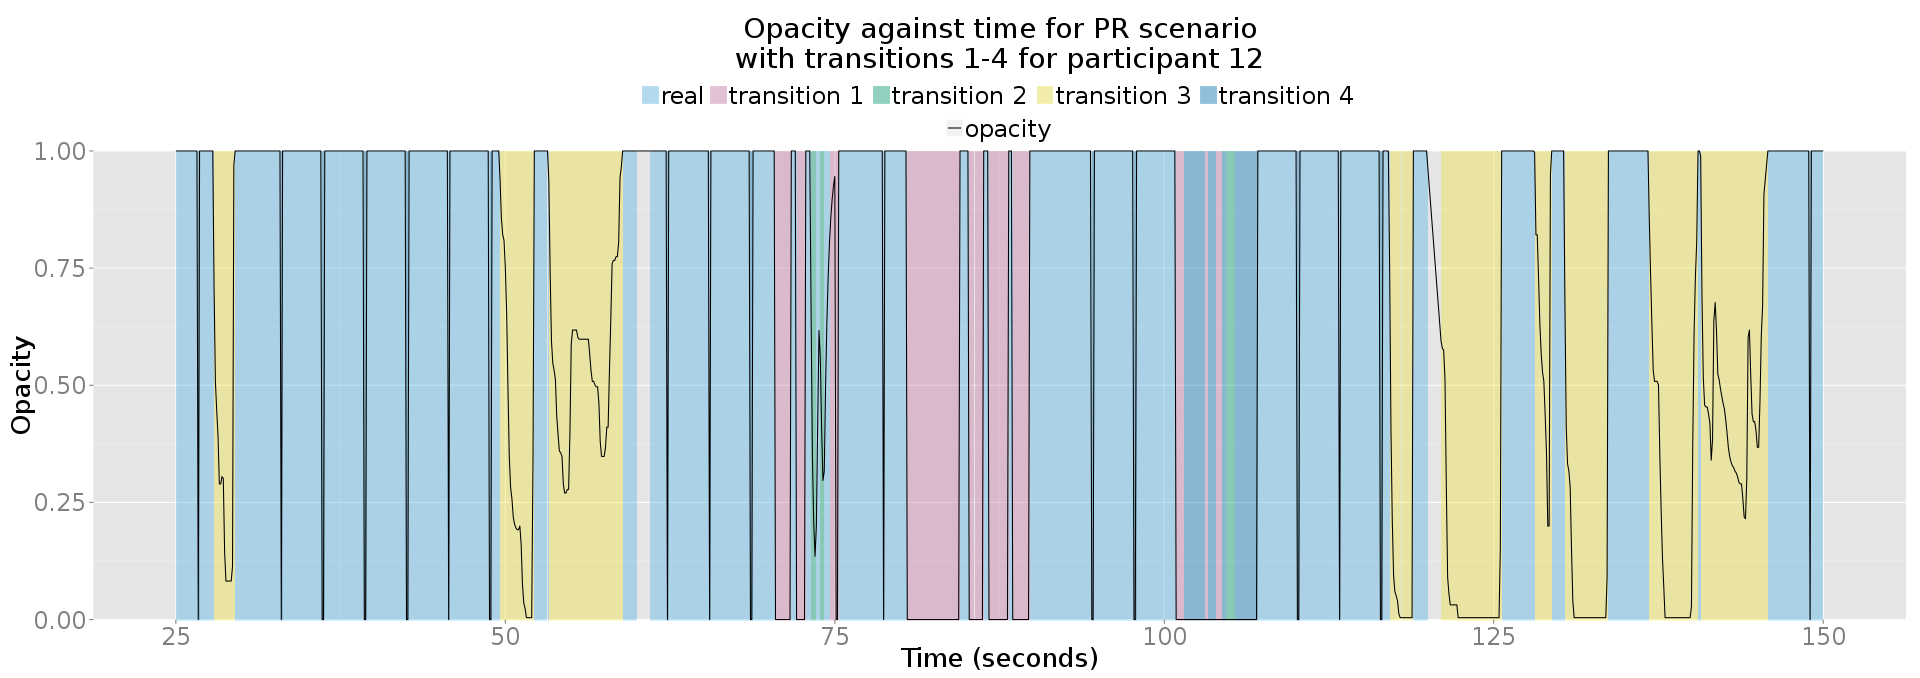
\includegraphics[width=\textwidth]{2.1/12-1-4_opacity.png}
	\caption{Opacity of camera objects against time for participant 12 in scenario 1-4, showing RW/VR transitions.}
	\label{12-1-4_opacity.png}
	\end{center}
\end{figure}

%=====================
	
%Other
%	participant 12 - all big head movements in 1-4 were in VR, but in 1-3 there was RW head movement too?


%Number of transitions in each session ranged from high teens to low sixties.

%Mean times spent in real/virtual are much closer than in stage 1.
%Time spent in virtual
%	participant 8 - more time spent in VR in 1-4 to avoid the automatic switch
%	participant 9 - more time spent in VR because of better understanding what they were meant to be doing (familiarity)


%four of seven participants spent more time in real than virtual in both 1-3 and 1-4
%	for three participants the ratio was closer in 1-4 than in 1-3 (avoiding transition 4?)
%	one spent more time in virtual than real in both 1-3 and 1-4
%	one spent more time in real in 1-3 and then more time in virtual tin 1-4 (familiarity?)

%=========================================================================================================

\subsection{IPQ}

IPQ results were scaled from the -3 to +3 range used by the questionnaires to the 0 to 6 range used to express results herein. The reversed items (SP2, INV3 and REAL1) had their results appropriately reversed. Tables \ref{sp-2-1-table}, \ref{inv-2-1-table} and \ref{real-2-1-table} show the mean and standard deviation for SP, INV and REAL respectively for the all of the scenarios (traditional VR scenario, scenario 1-3 and scenario 1-4).

The traditional VR scenario produced baseline IPQ results for a traditional HMD based VR experience in which RW stimuli are suppressed from the user. SP and INV results for this traditional VR scenario were relatively high, while the REAL results were low; this is not surprising, as the graphical quality of the VR chapel reconstruction used throughout the Mirrorshades evaluation was not stellar, partly as a result of having to intentionally reduce the level of detail in order to maintain acceptable framerates throughout the evaluations, thus it should come as no surprise that even though participants perceived bodily actions to be possible within the VR environment (high SP) and found incompatible RW stimuli well suppressed (high INV) that the realness of the VR environment was nonetheless lacking (low REAL). As one participant said during their interview, it felt real even though it didn't look it - \textit{``\ldots obviously it wasn't the same quality, but I still felt so immersed in it. Even though part of me would've known it wasn't real, most of it felt real even though it didn't look like it''}.

In both parallel reality scenarios SP and REAL were reduced equally by a small amount, whilst INV was reduced more substantially and with greater reduction for scenario 1-4 than for scenario 1-3. This meets the hypothesis that a positive parallel reality experience would result in noticeably reduced INV but without substantial reduction in SP and REAL. The reduced INV indicates that participants were more aware of RW stimuli, but the only marginally reduced SP indicates that their sense of presence in the VR environment did not drastically suffer and the only marginally reduced REAL indicates that the perceived realness of the VR environment did not substantially suffer from tandem observation with the equivalent vantage points into the (necessarily real) RW environment, although the parallel reality effect was evidently not positive enough to elicit heightened overall SP results as was hypothesized might happen from a stellar parallel reality experience.

Looking specifically at the results for SP3 and INV2 (table \ref{sp3-inv2-2-1-table}), they seem to be tied together as per Constantin's observation (see section \ref{igroup-presence-questionnaire-explanation}) for the traditional VR scenario and scenario 1-3 where they fall equally. However in scenario 1-4, INV2 drops substantially more than SP3 which climbs to above its level in scenario 1-3. This lends support to the notion that in a parallel reality experience in which the user is encouraged (or forced, in the case of scenario 1-4 which featured transition 4) to view visual stimuli from two compatible environments that SP can be maintained, that the break in presence associated with a transition from one environment to the other is not so great as to effect a Gestalt switch and throw off perceptual/concrete processing to an extent that sense of presence (in terms of focus of atttention) is drastically reduced.

\begin{table}
\begin{center}
\begin{minipage}[t]{.45\linewidth}
\begin{center}
\begin{tabularx}{\textwidth}{c *{3}{>{\centering\arraybackslash}X}}
\toprule

\textbf{Scenario} & \textbf{Mean} & \textbf{Standard deviation} \\

\midrule

traditional & 4.6 & 0.780 \\

1-3 & 4.133 & 1.093 \\

1-4 & 4.133 & 0.532 \\

\bottomrule
\end{tabularx}
\caption{Means and standard deviations of SP for all stage 2.1 scenarios.}
\label{sp-2-1-table}
\end{center}
\end{minipage}
%
\begin{minipage}[t]{.02\linewidth}
\hfill%
\end{minipage}
%
\begin{minipage}[t]{.45\linewidth}
\begin{center}
\begin{tabularx}{\textwidth}{c *{3}{>{\centering\arraybackslash}X}}
\toprule

\textbf{Scenario} & \textbf{Mean} & \textbf{Standard deviation} \\

\midrule

traditional & 4.166 & 1.393 \\

1-3 & 2.666 & 1.125 \\

1-4 & 1.958 & 1.308 \\

\bottomrule
\end{tabularx}
\caption{Means and standard deviations of INV for all stage 2.1 scenarios.}
\label{inv-2-1-table}
\end{center}
\end{minipage}

\vspace{5mm}

\begin{minipage}[t]{.45\linewidth}
\begin{center}
\begin{tabularx}{\textwidth}{c *{3}{>{\centering\arraybackslash}X}}
\toprule

\textbf{Scenario} & \textbf{Mean} & \textbf{Standard deviation} \\

\midrule

traditional & 2.208 & 1.134 \\

1-3 & 1.917 & 1.339 \\

1-4 & 1.917 & 1.080 \\

\bottomrule
\end{tabularx}
\caption{Means and standard deviations of REAL for all stage 2.1 scenarios.}
\label{real-2-1-table}
\end{center}
\end{minipage}
%
\begin{minipage}[t]{.02\linewidth}
\hfill%
\end{minipage}
%
\begin{minipage}[t]{.45\linewidth}
\begin{center}
\begin{tabularx}{\textwidth}{c *{5}{>{\centering\arraybackslash}X}}
\toprule

\textbf{Scenario} & \multicolumn{2}{c}{\textbf{SP3}} & \multicolumn{2}{c}{\textbf{INV2}} \\

\cmidrule(l){2-3} \cmidrule(l){4-5}

 & \textbf{mean} & \textbf{sd} & \textbf{mean} & \textbf{sd} \\
 
\midrule

traditional & 4.5 & 1.472 & 4 & 1.673 \\

1-3 & 2.5 & 2.160 & 2.8 & 1.643 \\

1-4 & 3.5 & 1.633 & 1 & 0.707 \\
 
\bottomrule
\end{tabularx}
\caption{Means for SP3 and INV2 for all stage 2.1 scenarios.}
\label{sp3-inv2-2-1-table}
\end{center}
\end{minipage}
\end{center}
\end{table}

%=========================================================================================================

\subsection{Stage 2.1 Summary}

This stage of the evaluation has provided first insight into best practices for implementing future parallel reality experiences. The ability to manually control the balance of RW/VR visuals has emerged as preferable to more basic transitions that simply alternate between the extremes of 100\% RW and 100\% VR, while adding uncontrolled VR visuals to the default view led to a negative effect upon enjoyment and comfort but a positive effect upon observation and understanding of the relationship between the two constituent environments.

Participants overwhelmingly preferred transition 3 compared to the others, which was somewhat surprising as initial experiments with the Mirrorshades platform with members of the OVW research group strongly indicated preference toward transition 2. With the larger number of participants in this stage of evaluation and the relatively unscientific nature of the tests within the OVW group, this preference toward transition 3 should be considered legitimate even though unexpected. Reasoning for preference toward transition 3 included being able to see both environments at once and a heightened sense of control.

Transition 4 was unanimously negatively received in terms of overall comfort and enjoyment of the scenarios, however participants did comment on heightened awareness and understanding between the two environments when transition 4 was present. Comments from participants concerning transition 4 such as that each time it occurred they would need to \textit{``stop and work it out again''} directly supports the notion that transition 4 results in a larger break in presence, in terms of movement on the focus of attention axis from presence toward absence, than the the other transition styles, with `working it out' alluding to the notion of conceptual/abstract reasoning that sits opposite perceptual/concrete processing at the two ends of the balance of focus of attention.

One relationship that did not arise as expected was a preference toward different transition styles in different situations, such as using transition 1 when performing a quick check on the VR environment and transition 3 when performing a more in-depth comparison. Instead it seems that most participants `experimented' with the transition styles available to them and settled upon a favourite, then used that one style throughout the rest of the scenario. Either the difference in utility between the different transition styles was not great enough to prompt participants to consider using different styles in different situations, or comfort trumped utility and participants continued to use the transition style they found most comfortable even if they thought that another might have served them better for a specific set of circumstances.

The same relationships with head movement as seen in stage 1 returned for stage 2.1, with substantially more variance in yaw than pitch across all scenarios, more variance in head movement when perceiving VR than RW during the parallel reality scenarios and more variance in head movement while standing stationary than when walking during the parallel reality scenarios.

IPQ results met hypotheses, with the traditional VR scenario scoring highly in both SP and INV while scoring lowly in REAL (explained by the low visual quality of the VR model) and the parallel reality scenarios only marginally reducing SP and REAL while more substantially reducing INV. Of particular interest is that scenario 1-4 displayed a substantial gap between SP3 and INV2, whereas with scenario 1-3 these values were reduced more evenly from the traditional VR scenario baseline. These IPQ results indicate that the parallel reality scenarios undertaken by stage 2.1 participants succeed in allowing participants to experience the RW environment in tandem with the VR environment, without having a substantial negative effect upon their sense of presence in the VR environment or upon the perceived realism of the VR environment.

%=========================================================================================================

\clearpage

%=========================================================================================================

\section{Stage 2.2 - Default Views}

One of the threads that emerged from the stage 2.1 investigation was that while transition 4 was unanimously negatively received because of the worse breaks in presence that it caused by `surprising' the participants, the VR visual stimuli that it presented without participants having to consciously trigger a transition led to several participants indicating that it resulted in them better understanding the relationship between the two environments and noticing more differences between them. Stage 2.2 thus investigated how untriggered VR stimuli could be introduced into a parallel reality experience but in a less obtrusive manner than transition 4, namely by changing the default view to less than 100\% RW.

Stage 2.2 followed the same basic pattern as stage 2.1, with participants engaging in a traditional VR scenario in which they were seated and used the DK1 and Xbox controller to explore the VR chapel in addition to engaging in two parallel reality scenarios in which they walked through the chapels, once again completing three scenarios in total;

\begin{enumerate}
	\item \textbf{Traditional VR scenario} - Participants explore the VR chapel from a stationary position, as VR has traditionally been employed at cultural heritage sites via CAVE installations and by the OVW group with Oculus HMDs, using the Xbox controller to move around the VR environment observed via the DK1, with the DK1 obscuring theier view of the RW chapel around them.
	\item \textbf{PR scenario with 75\% RW/25\% VR default view} - (Referred to as the `75/25 scenario') Participants experience the RW and VR chapels in tandem using the Mirrorshades platform. They wear the DK1, holding the Xbox controller in their right hand and the smartphone in their left, with the laptop and control box bundle in a satchel worn over one shoulder. The default view on the DK1 screen is 75\% RW/25\% VR, achieved by setting the base opacity of the objects upon which the camera feeds are rendered to 75\%. The participants are furnished with a single transition style, the transition with linear interpolation (transition 2 from the stage 2.1 evaluation).
	\item \textbf{PR scenario with 50\% RW/50\% VR default view} - (Referred to as the `50/50 scenario') Participants undertake the same scenario as the 75/25 scenario, except the default view on the DK1 screen is 50\% RW/50\% VR, achieved by setting the base opacity of the objects upon which the camera feeds are rendered to 50\%. Participants are again fashioned with the linear interpolated transition as the only transition style.
\end{enumerate}

As the controlled variable between the two parallel reality scenarios was opacity based, it seemed prudent not to fashion the participants with the ability to consciously affect opacity by giving them access to the analogue selectable opacity feature (transition 3 from the stage 2.1 evaluation). In the same manner as during stage 2.1, participants were simply instructed to make their way from the starting position down to the altar end of the chapel, with no hard restrictions upon their path or when/where they were to stop and pay attention to particular aspects of their surroundings.

%=========================================================================================================

\section{Stage 2.2 Results}

A total of 4 participants completed the stage 2.2 evaluation;
\begin{itemize}
	\item Age ranged from 19 to 38, with a mean of 24.3 and a standard deviation of 9.2
	\item 2x identified as male and 2x as female
	\item 3x reported previous experience with a games console controller
	\item None reported previous experience with a HMD
	\item 1x reported having previously visited the chapel
	\item None reported having previously experienced the virtual chapel
\end{itemize}

%=========================================================================================================

\subsection{Likert-type Questionnaires}

When considering the responses to the Likert-type questionnaires (see figure \ref{9-item-likert-type-questionnaire.png}) for the two parallel reality scenarios of the stage 2.2 evaluation, the following observations can be made.

\begin{figure}[h]
	\begin{center}
	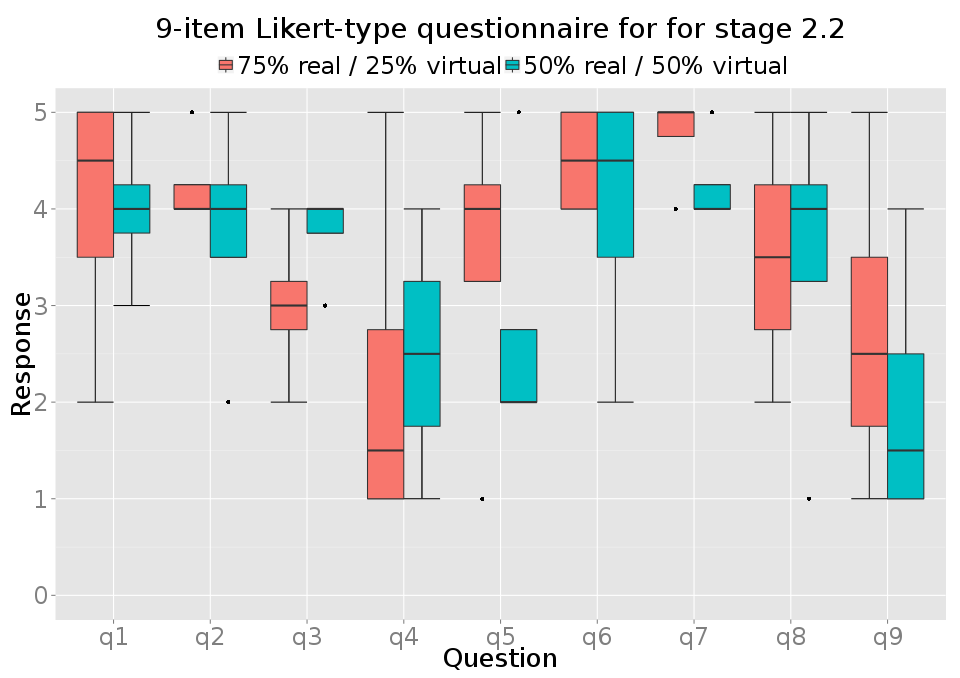
\includegraphics[width=.6\textwidth]{2.2/9-item-likert-type-questionnaire.png}
	\caption{Stage 2.2 evaluation Likert-type questionnaire results.}
	\label{9-item-likert-type-questionnaire.png}
	\end{center}
\end{figure}

\begin{itemize}
	\item Participants overall preferred the 75/25 scenario over the 50/50 scenario (q1)
	\item Participants found it easier to compare features from past and present in the 50/50 scenario than the 75/25 scenario (q3)
	\item Participants experienced more motion sickness in the 75/25 scenario than in the 50/50 scenario (q5)
	\item The 50/50 scenario was reported as being less rewarding for exploring the chapel than the 75/25 scenario (q6)
	\item Participants thought that they did not notice differences between real and virtual more in the 75/25 scenario than in the 50/50 scenario (q9)
\end{itemize}

%=========================================================================================================

\subsection{Interview Transcripts}

Once again, the interview recordings that were transcribed after the chapel sessions gave valuable insight into the experience of the two parallel reality scenarios in stage 2.2.

Two participants said that they preferred the 75/25 scenario, while the other two participants preferred the 50/50 scenario. Of those that preferred the 75/25 scenario, one explained that s/he felt more in control of whether s/he was seeing real or virtual while the other found the more obvious sudden VR movements visible during the 50/50 scenario to be uncomfortable. Of those that preferred the 50/50 scenario one reported that of the 75/25 scenario that it was \textit{``confusing to make sense of what I was seeing''} while the other found that switching to fully VR was less of a jump coming from 50/50, alluding to a less severe break in presence, thus was \textit{``more comfortable spending more time in the virtual''}. One participant directly answered that they thought they used the button to manually transition more in the 50/50 scenario because it was less jarring than in the 75/25 scenario.

All of the participants however reported that the 50/50 scenario was more engaging. Interestingly, one of the participants who reported preferring the 75/25 scenario largely because of inaccuracy of the IPS during the 50/50 scenario to cause disorientation, commented that this inaccuracy led to greater engagement because it would show him/her other parts of the VR chapel than were equivalent to his/her immediate surroundings (akin to Briand's `controlled schizophrenia' (see section \ref{the-mirrorshades-platform}) but completely unintentional). Two participants further reported that the 50/50 scenario made differences between RW and VR more obvious, with one reporting not much discernible difference. One participant specifically mentioned how the 50/50 scenario made it more \textit{``perceptible exactly where things were''} which led to seeing him/herself \textit{``walking through''} (virtual) things whereas with the 75/25 scenario s/he would have to \textit{``switch back and forth and then realise''}.

Mimicking responses from earlier stage interviews, one participant reported experiencing motion sickness during the traditional VR scenario when using the Xbox controller stick to turn, while when considering the parallel reality scenarios three of the four participants reported less motion sickness during the 50/50 scenario.

%=========================================================================================================

\subsection{Log Data}

\subsubsection{Considering all scenarios (traditional and PR)}

Once again, variance in yaw dominated for all participants during all three scenarios (traditional and both parallel reality scenarios) over variance in pitch, which is illustrated in figure \ref{14-pitch-yaw-trad-75-25-50-50.png} which shows pitch and yaw against time for participant 14 for the traditional VR scenario at left, the 75/25 scenario in the middle and the 50/50 scenario on the right (note that the 75/25 scenario is of substantially longer duration than the other two scenarios, thus the marked difference in initial appearance).

\begin{figure}[h]
	\begin{center}
	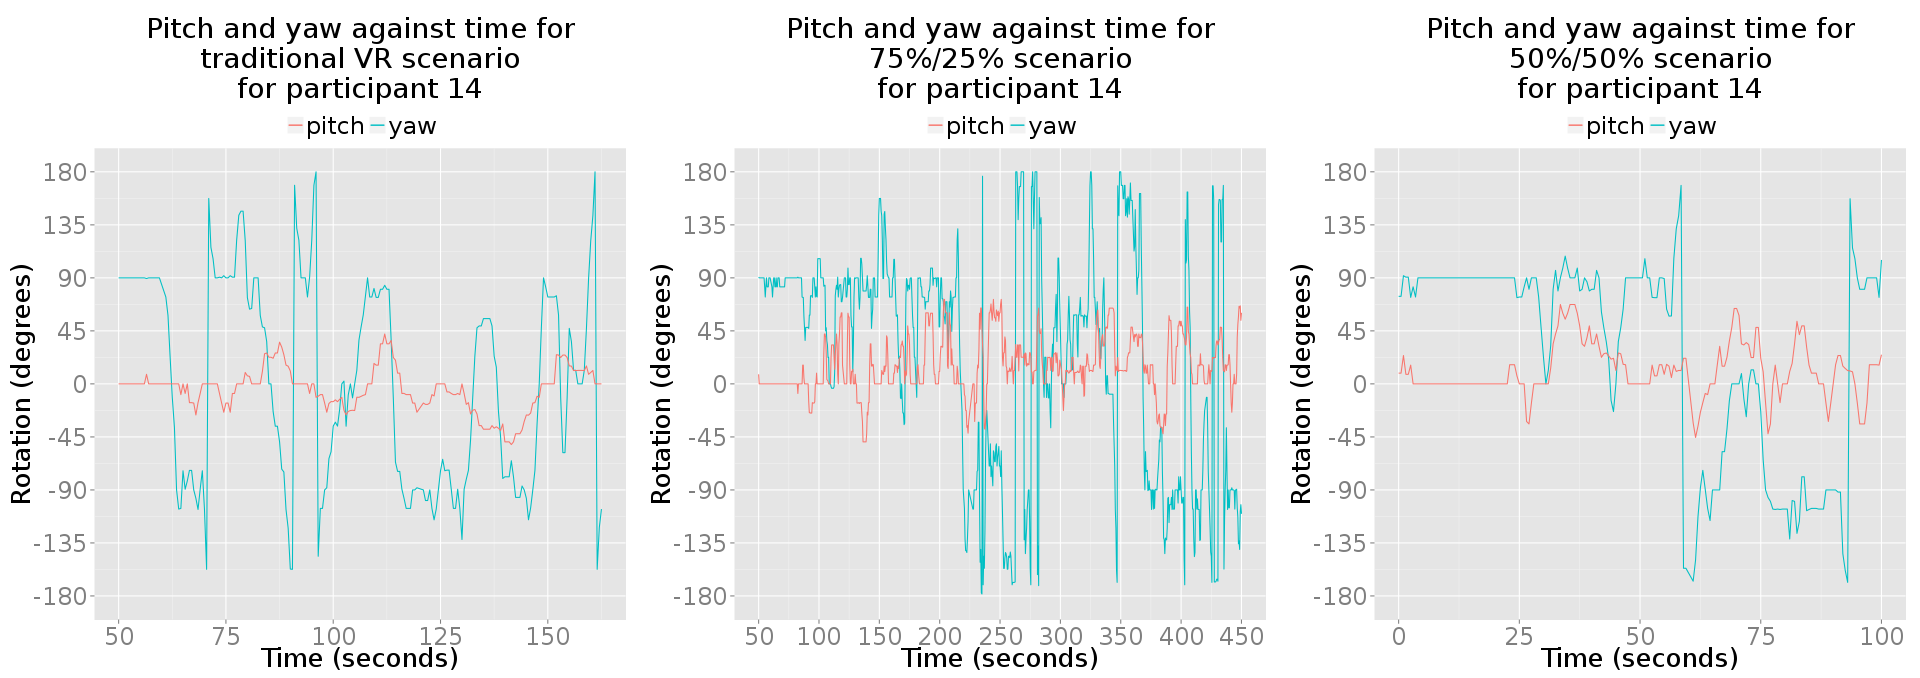
\includegraphics[width=\textwidth]{2.2/14-pitch-yaw-trad-75-25-50-50.png}
	\caption{Pitch and yaw against time for participant 14 in traditional and both parallel reality scenarios.}
	\label{14-pitch-yaw-trad-75-25-50-50.png}
	\end{center}
\end{figure}

%=====================

\subsubsection{Comparing Between 75/25 and 50/50 Scenario}

The main new observations that come to light when comparing log data for the two parallel reality scenarios are that all of the participants performed fewer transitions in the 50/50 scenario than in the 75/25 scenario, with three of the participants also spending more time (both overall and in terms of the average duration of the periods) perceiving the default position rather than VR in the 75/25 scenario than the 50/50 scenario. These values are summarised in tables \ref{times-75-25} and \ref{times-50-50} for the 75/25 and 50/50 scenarios respectively, while figures \ref{16-pitch-yaw-75-25.png} and \ref{16-pitch-yaw-50-50.png} visualise this relationship for participant 16 performing the 75/25 scenario and 50/50 scenario respectively.

\begin{figure}[h]
	\begin{center}
	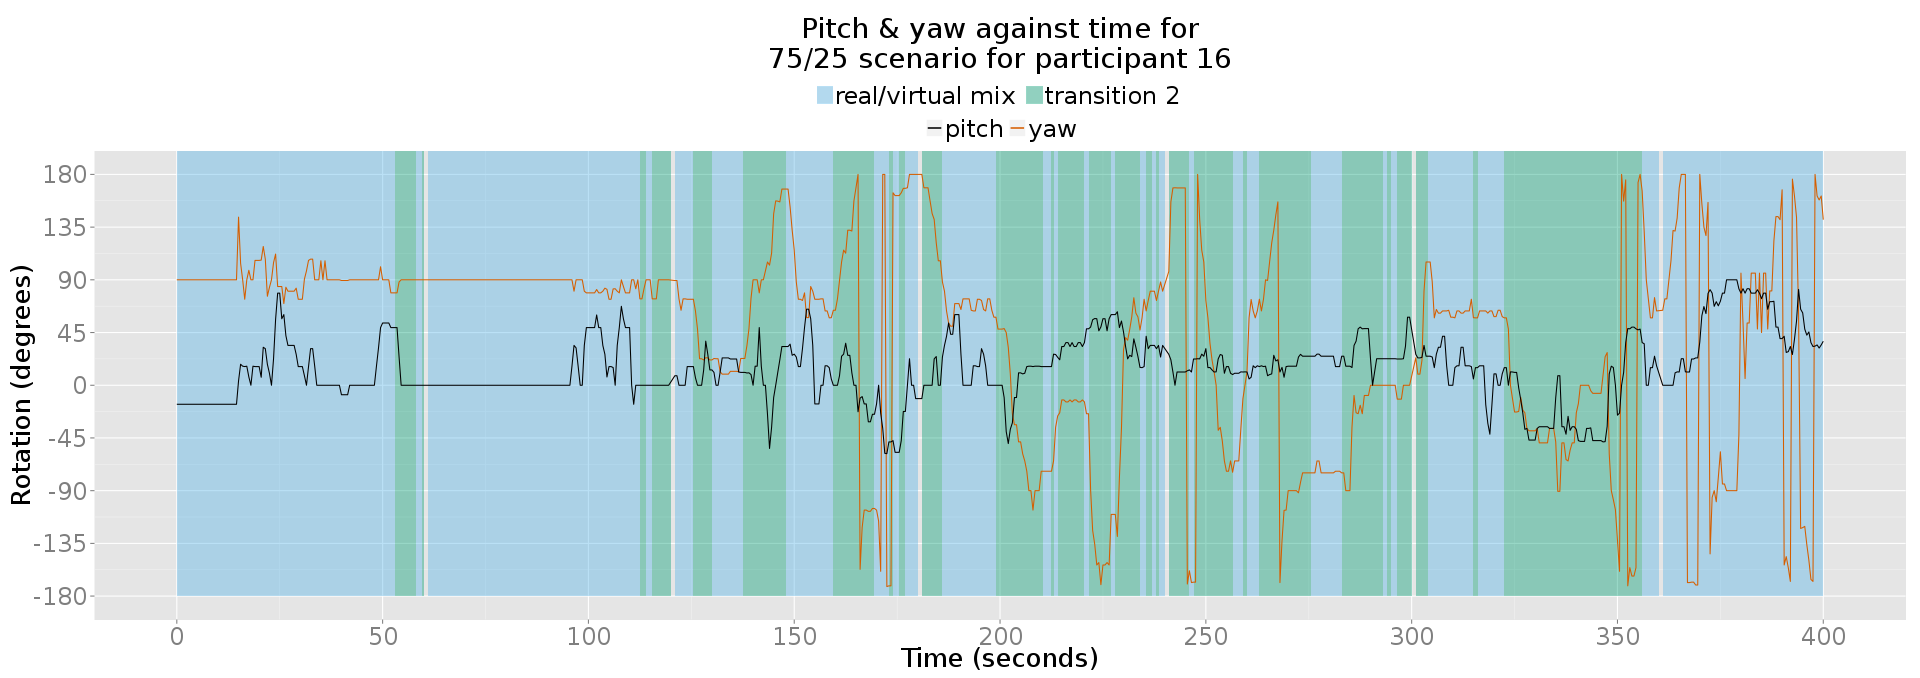
\includegraphics[width=\textwidth]{2.2/16-pitch-yaw-75-25.png}
	\caption{Pitch and yaw against time for participant 16 in 75/25 scenario, showing default/VR transitions.}
	\label{16-pitch-yaw-75-25.png}
	\end{center}
\end{figure}

\begin{figure}[h]
	\begin{center}
	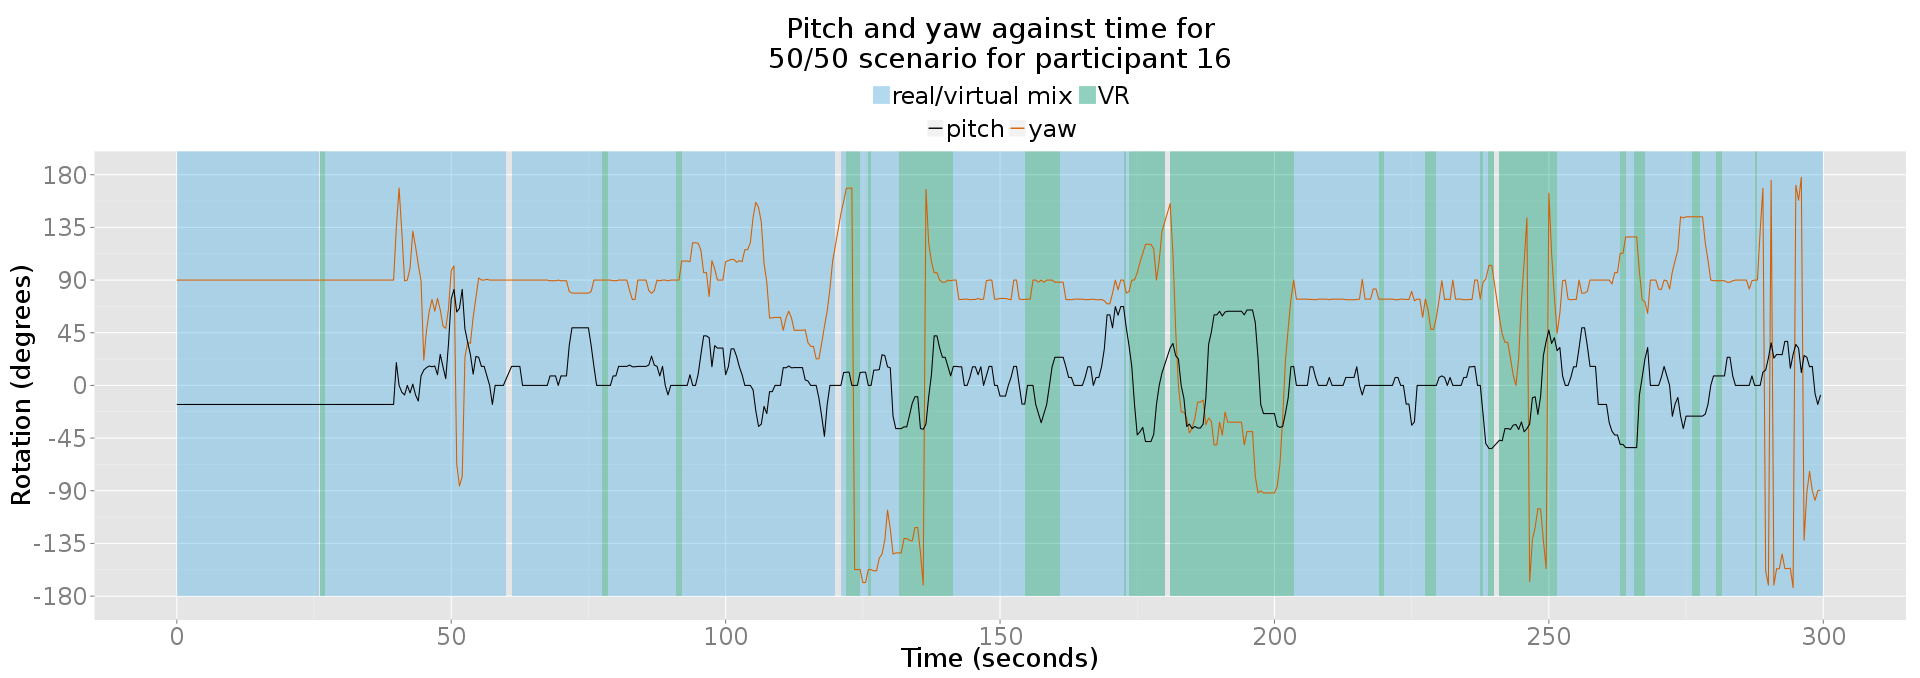
\includegraphics[width=\textwidth]{2.2/16-pitch-yaw-50-50.png}
	\caption{Pitch and yaw against time for participant 16 in 50/50 scenario, showing default/VR transitions.}
	\label{16-pitch-yaw-50-50.png}
	\end{center}
\end{figure}

\begin{table}
\begin{center}
\begin{tabularx}{\textwidth}{c *{6}{>{\centering\arraybackslash}X}}
\toprule

\textbf{Participant} & \textbf{Number of transitions} & \multicolumn{2}{c}{\textbf{Mean duration (seconds)}} & \multicolumn{2}{c}{\textbf{Total duration (seconds)}} \\

\cmidrule(l){3-4} \cmidrule(l){5-6}

 & & \textbf{default} & \textbf{VR} & \textbf{default} & \textbf{VR} \\

\midrule

14 & 18 & 17.368 & 2.889 & 330 & 52 \\

15 & 15 & 14.656 & 3.233 & 234.5 & 48.5 \\

16 & 26 & 8.352 & 5.538 & 225.5 & 144 \\

17 & 15 & 5.013 & 1.2 & 80.2 & 18 \\

\bottomrule
\end{tabularx}
\caption{Distribution of time spent in default and VR environments for all participants during 75/25 scenario.}
\label{times-75-25}
\end{center}
\end{table}

\begin{table}
\begin{center}
\begin{tabularx}{\textwidth}{c *{6}{>{\centering\arraybackslash}X}}
\toprule

\textbf{Participant} & \textbf{Number of transitions} & \multicolumn{2}{c}{\textbf{Mean duration (seconds)}} & \multicolumn{2}{c}{\textbf{Total duration (seconds)}} \\

\cmidrule(l){3-4} \cmidrule(l){5-6}

 &  & \textbf{default} & \textbf{VR} & \textbf{default} & \textbf{VR} \\

\midrule

14 & 2 & 32.5 & \textless 1 & 97.55 & \textless 1 \\

15 & 12 & 9.077 & 2.542 & 118 & 30.5 \\

16 & 18 & 11.316 & 3.661 & 215 & 65.9 \\

17 & 6 & 19.714 & 0.167 & 138 & \textless 1 \\

\bottomrule
\end{tabularx}
\caption{Distribution of time spent in default and VR environments for all participants during 50/50 scenario.}
\label{times-50-50}
\end{center}
\end{table}

In combination with interview feedback, these log data support the notion that the 50/50 scenario was more engaging, with participants not finding it necessary to perform transitions to VR as frequently in order to perceive enough VR stimuli to engage with the combined RW and VR content.

When considering the distribution of variance in head pitch and yaw in relation to whether participants were viewing the default position or VR, maximum variance in stage 2.2 was no longer as restricted to the VR periods. Participant 14 in particular frequently displayed maximum variance when viewing the default position, more so even than when viewing VR, as shown by figure \ref{14-pitch-yaw-75_25.png}. While this is understandable in the sense that the participants no longer needed to perform a transition to VR in order to see the VR environment, it is also worth highlighting that by allowing the user to see the VR environment in this manner means that they were simultaneously perceiving more angles of the RW environment which in earlier stages of evaluation they may not have seen as maximum variance in pitch and yaw only occurred when they were viewing predominantly VR visual stimuli via the DK1.

\begin{figure}[h]
	\begin{center}
	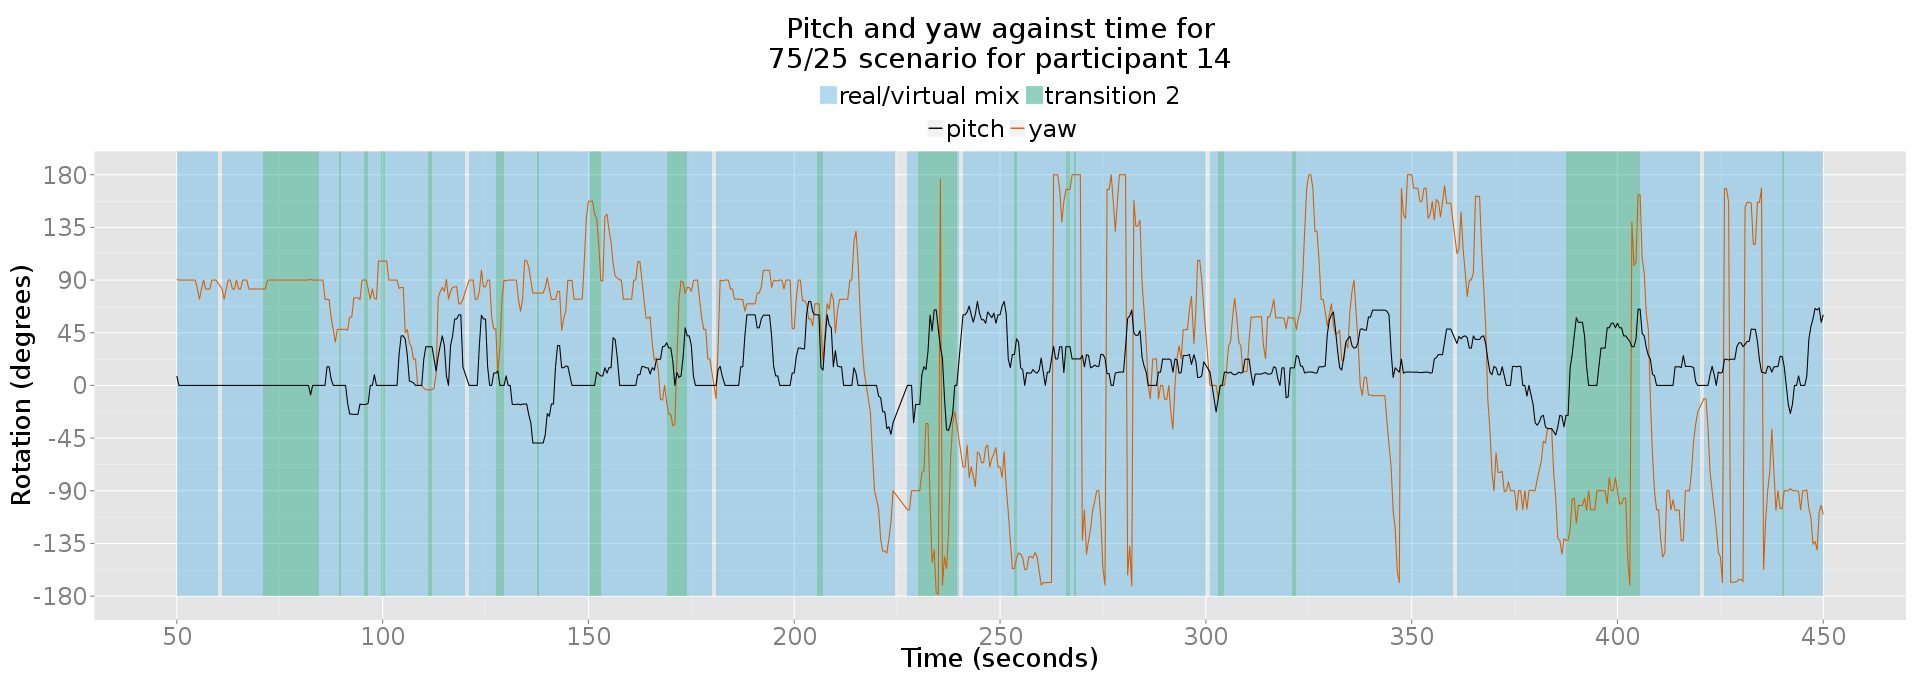
\includegraphics[width=\textwidth]{2.2/14-pitch-yaw-75_25.png}
	\caption{Pitch and yaw against time for participant 14 in 75/25 scenario, showing default/VR transitions.}
	\label{14-pitch-yaw-75_25.png}
	\end{center}
\end{figure}

%=====================

\subsubsection{Walking and Head Movement}

Concerning the relationship between variance in pitch and yaw compared to whether participants were actively walking, most participants exhibited similar behaviour to previous stages of evaluation with maximum variance restricted to periods in which they were standing still.

However as can be seen in figure \ref{17-pitch-yaw-distance-moved-75-25.png} participant 17 exhibited extremely restricted head movement, only moving their head from looking straight ahead in the direction of moment upon reaching the altar end of the chapel and turning around to return. Intuitively one might suppose that for a participant who did not feel sure of themselves when walking with the apparatus, not having a 100\% RW view may have resulted in this static head behaviour as they needed to focus all of their attention on what lessened amount of the RW environment they could see in order to successfully navigate. However this participant did not report any such lack of surety in the interview, although did mention performing fewer transitions in the 50/50 scenario as they were \textit{``trying to make sure I didn't bump into anything''} and reviewing the video recording of this participant completing the 75/25 scenario showed them to walk comfortably and deliberately. Thus the mostly static head activity is as likely to be attributable to simple disinterest with the environments or misunderstanding of the purpose of the scenarios as due to any restricting aspect of the apparatus or experience.

\begin{figure}[h]
	\begin{center}
	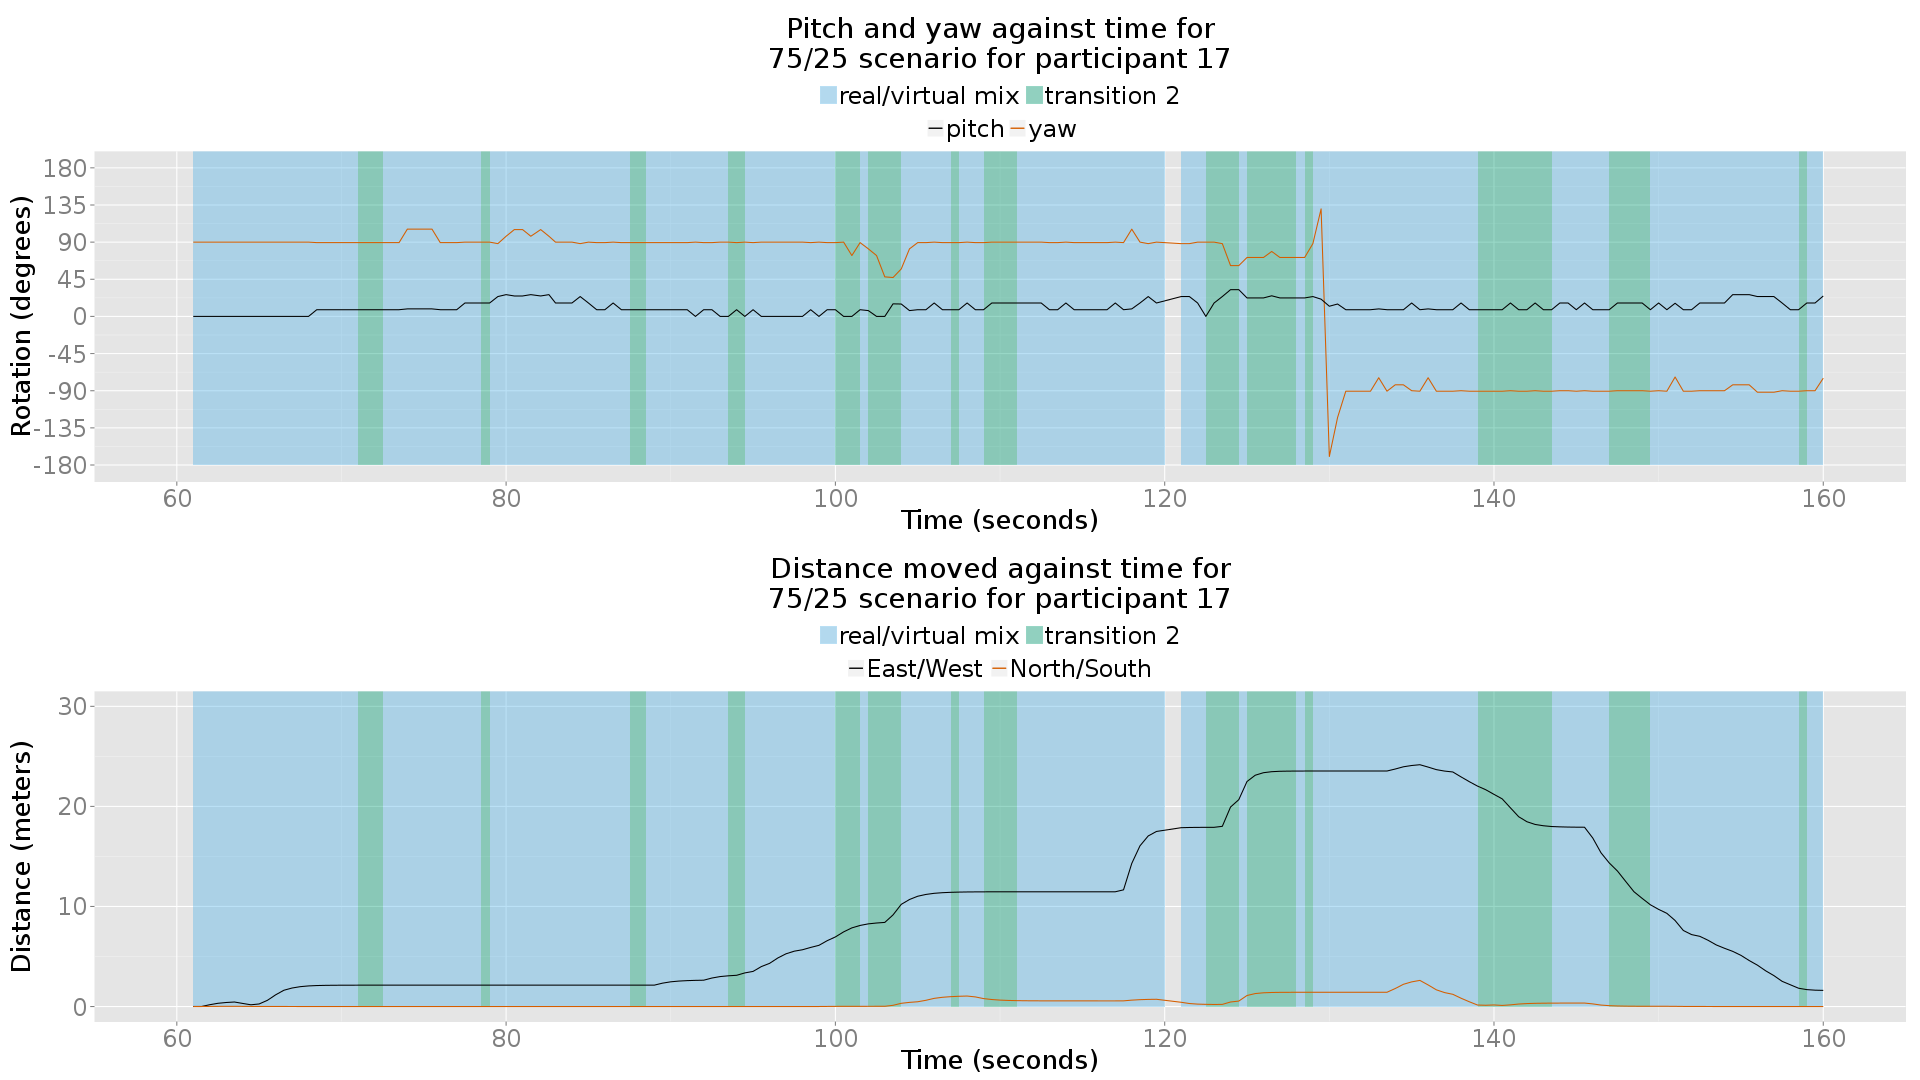
\includegraphics[width=\textwidth]{2.2/17-pitch-yaw-distance-moved-75-25.png}
	\caption{Pitch and yaw against time aligned with distance moved against time for participant 17 in 75/25 scenario, showing default/VR transitions.}
	\label{17-pitch-yaw-distance-moved-75-25.png}
	\end{center}
\end{figure}

%=========================================================================================================

\subsection{IPQ}

When considering the IPQ results for stage 2.2 participants the traditional VR scenario presents very similar results for all of SP, INV and REAL (tables \ref{sp-2-2-table}, \ref{inv-2-2-table} and \ref{real-2-2-table} respectively) to the traditional VR scenario from stage 2.1 (tables \ref{sp-2-1-table}, \ref{inv-2-1-table} and \ref{real-2-1-table}), which was to be expected and confirms these values as good baseline IPQ results for a traditional VR experience at the chapel.

SP was reduced in the 75/25 scenario, to a level slightly lower than that in both parallel reality scenarios in stage 2.1, while in the 50/50 scenario there was a marked increase in SP to a level (4.7) above any other scenario in either stage, including the traditional VR scenarios. This hints toward the optimistic expectation of a good parallel reality experience resulting in reduced INV but increased SP compared to a traditional VR scenario, by representation of bodily actions within the RW environment leading to an increase in experienced spatial presence within the VR environment.

INV was reduced in the 75/25 scenario and further reduced in the 50/50 scenario, as was to be expected. Interestingly however, the INV results for both parallel reality scenarios in stage 2.2 were notably higher than those for the parallel reality scenarios of stage 2.1, a discrepancy that is not contained within the higher INV for the traditional VR scenario in stage 2.2 compared to stage 2.1.

REAL was reduced in the 75/25 scenario to almost exactly the same level as both parallel reality scenarios in stage 2.1, however for the 50/50 scenario REAL was only reduced a miniscule amount (a reduction of 0.118 from 2.563 to 2.438). This implies that the increased visibility of the VR environment when perceiving the RW environment helped to enhance the perceived realness of the VR environment.

When considering SP3 and INV2 in isolation, the mean SP3 for the traditional VR scenario is confusingly low at 1.75 (table \ref{sp3-inv2-2-2-table}). This is especially odd considering the relatively high mean for the overall SP subscale in the traditional VR scenario of 4.3 (table \ref{sp-2-2-table}). It is also completely out of line with the mean SP3 for the traditional VR scenario from stage 2.1 of 4.5 (table \ref{sp-2-1-table}), which was in keeping with the overall SP mean of 4.6 (table \ref{sp3-inv2-2-1-table}) for the traditional VR scenario in stage 2.1. This oddity could be explained by possible confusion among the stage 2.2 participants over the wording of SP3, which presents a negative - \textit{``I did \textbf{not} feel present in the virtual space''} (emphasis added), anchored between \textit{``did not feel''} and \textit{``felt present''}.

\begin{table}
\begin{center}
\begin{minipage}[t]{.45\linewidth}
\begin{center}
\begin{tabularx}{\textwidth}{c *{3}{>{\centering\arraybackslash}X}}
\toprule

\textbf{Scenario} & \textbf{Mean} & \textbf{Standard deviation} \\

\midrule

traditional & 4.3 & 0.476 \\

75/25 & 3.95 & 1.248 \\

50/50 & 4.7 & 0.739 \\

\bottomrule
\end{tabularx}
\caption{Means and standard deviations of SP for all stage 2.2 scenarios.}
\label{sp-2-2-table}
\end{center}
\end{minipage}
%
\begin{minipage}[t]{.02\linewidth}
\hfill%
\end{minipage}
%
\begin{minipage}[t]{.45\linewidth}
\begin{center}
\begin{tabularx}{\textwidth}{c *{3}{>{\centering\arraybackslash}X}}
\toprule

\textbf{Scenario} & \textbf{Mean} & \textbf{Standard deviation} \\

\midrule

traditional & 4.625 & 1.299 \\

75/25 & 4.25 & 1.594 \\

50/50 & 3.25 & 1.696 \\

\bottomrule
\end{tabularx}
\caption{Means and standard deviations of INV for all stage 2.2 scenarios.}
\label{inv-2-2-table}
\end{center}
\end{minipage}

\vspace{5mm}

\begin{minipage}[t]{.45\linewidth}
\begin{center}
\begin{tabularx}{\textwidth}{c *{3}{>{\centering\arraybackslash}X}}
\toprule

\textbf{Scenario} & \textbf{Mean} & \textbf{Standard deviation} \\

\midrule

traditional & 2.563 & 1.56 \\

75/25 & 1.938 & 1.593 \\

50/50 & 2.438 & 1.360 \\

\bottomrule
\end{tabularx}
\caption{Means and standard deviations of REAL for all stage 2.2 scenarios.}
\label{real-2-2-table}
\end{center}
\end{minipage}
%
\begin{minipage}[t]{.02\linewidth}
\hfill%
\end{minipage}
%
\begin{minipage}[t]{.45\linewidth}
\begin{center}
\begin{tabularx}{\textwidth}{c *{5}{>{\centering\arraybackslash}X}}
\toprule

\textbf{Scenario} & \multicolumn{2}{c}{\textbf{SP3}} & \multicolumn{2}{c}{\textbf{INV2}} \\

\cmidrule(l){2-3} \cmidrule(l){4-5}

 & \textbf{mean} & \textbf{sd} & \textbf{mean} & \textbf{sd} \\
 
\midrule

traditional & 1.75 & 2.217 & 5 & 0.816 \\

75/25 & 3.75 & 1.708 & 3.5 & 1.732 \\

50/50 & 5.25 & 0.957 & 3.75 & 1.893 \\
 
\bottomrule
\end{tabularx}
\caption{Means for SP3 and INV2 for all stage 2.2 scenarios.}
\label{sp3-inv2-2-2-table}
\end{center}
\end{minipage}
\end{center}
\end{table}

%=========================================================================================================

\subsection{Stage 2.2 Summary}

This stage of the evaluation investigated the effects of changing the default view of a parallel reality scenario to one that always includes some aspect of the VR environment, such that the user is at all times receiving some degree of VR stimuli even when they do not consciously trigger a transition into a non-default view and without relying upon a severe break in presence causing instantaneous transition to and from a 100\% VR view as was the case with transition 4 in the second of the stage 2.1 parallel reality scenarios.

Comparing the parallel reality scenarios from this stage of the evaluation to the second parallel reality scenario from the stage 2.1 evaluation in which transition 4 was used, the IPQ results indicate that the 75/25 scenario reduced SP and REAL to similar levels however the 50/50 scenario resulted in an almost imperceptible decrease in REAL and a noticeable \textit{increase} in SP, while the results for the traditional VR scenario closely matched those from the stage 2.1 evaluation.

Despite these results and the fact that the 50/50 scenario was reported as allowing easier comparison between the two environments, it was considered less rewarding and was less preferred overall compared to the 75/25 scenario. In some ways this mimics the relationship between the first stage 2.1 parallel reality scenario and the second stage 2.1 parallel reality scenario, where although the second led to furthered understanding of the two environments it did so at a cost of comfort and enjoyment.

Fewer transitions overall during the 50/50 scenario with participants spending more time in total and per transition viewing the VR environment in scenario 75/25 supports the notion that with an increased amount of VR visible in the default position that participants did not perceive the necessity to perform a conscious transition to see VR content that interested them. Considering the relationship observed in the stage 2.1 parallel reality scenarios of maximum variance of head movement restricted to periods in which the participants were viewing 100\% VR, reducing the participants' reliance upon performing these transitions stands to benefit participants' observation of RW components that they would otherwise have missed by looking only at the VR environment when looking in certain directions.

However it is worth considering that while a default view that presents \textless 100\% RW does seem to increase participant exposure to angles of the RW environment other than those required to perceive when walking, by allowing users to look around at the VR environment when stationary without needing to perform a transition to 100\% VR and thus losing all visual stimuli from the RW environment, that for a participant who feels less comfortable walking with the apparatus that not having a 100\% RW view available will likely have a detrimental effect to the experience as a whole. Furthermore, if a user wishes to inspect something in the RW environment in particular detail, not being able to activate a 100\% RW view may well reduce their ability to discern detail in this object, again hampering the overall parallel reality experience. Although this stage 2.2 evaluation prevented users from occupying a position at the RW extreme of the locus of attention axis by always showing them at least 25\% or 50\% of the VR environment, this is not strictly a sensible approach. A sensible approach for real world application would perhaps be to allow toggling between a 100\% RW view and one a (for example) 50/50 view, such that users could reap the benefits of the combined view but maintain the ability to transition back to a 100\% RW view and the RW extreme of the focus of attention axis when the situation demands it.

%=========================================================================================================

\section{Best Practices for PR}

The evaluations described in this and the preceding chapter have experimentally shown the value of the Mirrorshades platform and parallel reality in general as a new modality for on-site comparison of real and immersive virtual environments within the context of a cultural heritage site, as well as revealing a number of indicators toward best practices for future implementation of parallel reality systems.

With the merit of the platform compared to a traditional VR experience established by the stage 1 evaluation, the second stage of evaluation explored different implementation details of the platform to inform future implementation of similar systems such that the benefits of the concept can be best exploited. Stage 2.1 assessed participant responses to several different styles of performing transitions between the constituent RW and VR environments, with a transition which furnished participants with complete control over the percentage of the visual stimuli of each environment that were presented to them emerging the clear favourite. The introduction of automatic transitions from RW to VR was met negatively when assessed in terms of enjoyment and preference, but positively when assessed in terms of awareness and understanding of the relationships between the two environments.

Stage 2.2 further investigated the concept of presentation of VR visual stimuli to the user without their conscious invocation of a transition, the intention being to raise awareness and understanding between the environments without introducing the negativity of the automatic transition, by replacing the 100\% RW default view of earlier stages with ones that presented a percentage of each environment at all times. The more extreme case of a 50/50 split led to the greater increase in spatial presence within the VR environment and a barely perceptible decrease in experienced realism of the RW environment, however the 75/25 split that led to a less remarkable change was preferred by the participants.

Considering these findings, several best practices for future parallel reality implementations are proposed;

\begin{enumerate}
	\item Both a 100\% RW and a 100\% VR view should be provided, though these do not have to be the default RW/VR positions. A 100\% VR view is diagnostic for situations in which the user wishes to perform deliberate in depth observations of a VR object, while a 100\% RW view is important both for performing the same observations of RW objects but also such that movement in the RW environment can be made as comfortable as possible for the user. Whilst improvements to HMDs and associated video see-through technologies, along with improvements to the accuracy of indoor positioning systems, will undoubtedly mitigate the detrimental effects of walking while using a HMD based parallel reality system such as Mirrorshades, the ability to revert to a 100\% RW view will ensure that the experience of walking in such a situation is presented at its most agreeable.
	\item A view that provides less than 100\% RW without the need to keep a control activated should be provided. Presenting VR visuals in this manner, such that the user receives VR stimuli even without consciously thinking to perform a transition to VR or a RW/VR mix, has shown to have a positive effect both upon participant awareness of the VR content and the relationship between this content and the RW environment and also promote observation of RW vantages that might otherwise only be seen through VR. The balance between RW and VR visuals in such a view needs to be carefully considered, as although reducing RW visuals more in the evaluations led to heightened awareness and understanding of the relationship between the environments, it was the less drastically reduced RW view that was preferred overall.
	\item A method of transitioning between default RW and VR positions that allows the user to both control the speed of the transition and to stop at any intermediary level between 100\%RW/0\%VR and 0\%RW/100\%VR should be provided. This style of transition was clearly the best received throughout the evaluations and participants often used this transition to pause at intermediary opacities.
\end{enumerate}

%=========================================================================================================